\documentclass[dissertacao]{inf-ufg}
%\usepackage{algorithm}
%\usepackage{algorithmic}
%\usepackage[portuguese]{algorithm2e}
\usepackage{pgfplots}
\usepackage{multicol}
\usepackage{multirow}
\usepgfplotslibrary{external}
\usepackage{pdfpages}
%\usepackage{minted}
\usepackage{tikz}
\usepackage{verbatim}
\usetikzlibrary{arrows,shapes,backgrounds,calc,snakes}
\usepgfplotslibrary{fillbetween}
\usepackage{pgfplotstable}
\usepackage{pdflscape}
\usepackage{multicol}
\usepackage{tabularx}
\usepackage{url}
\usepackage{hyperref}
\usepackage{algorithm}
\makeatletter 
\renewcommand\thealgorithm{\thechapter.\arabic{algorithm}} 
\@addtoreset{algorithm}{chapter} 
\makeatother

\newtheorem{observation}[definition]{Observação}
\newtheorem{properties}[definition]{Propriedades}
%\newtheorem{coro}{Corolário}
\newtheorem{coro}[definition]{Corolário}
\newtheorem{conjecture}[definition]{Conjectura}
\newcommand{\multicolinterrupt}[1]{% Stuff to span both rows
\SetKw{Interromper}{interromper}
\SetKw{Continue}{continue}
\end{multicols}
#1
\begin{multicols}{2}
}


\newcommand{\convexpath}[2]{
[   
    create hullnodes/.code={
        \global\edef\namelist{#1}
        \foreach [count=\counter] \nodename in \namelist {
            \global\edef\numberofnodes{\counter}
            \node at (\nodename) [draw=none,name=hullnode\counter] {};
        }
        \node at (hullnode\numberofnodes) [name=hullnode0,draw=none] {};
        \pgfmathtruncatemacro\lastnumber{\numberofnodes+1}
        \node at (hullnode1) [name=hullnode\lastnumber,draw=none] {};
    },
    create hullnodes
]
($(hullnode1)!#2!-90:(hullnode0)$)
\foreach [
    evaluate=\currentnode as \previousnode using \currentnode-1,
    evaluate=\currentnode as \nextnode using \currentnode+1
    ] \currentnode in {1,...,\numberofnodes} {
-- ($(hullnode\currentnode)!#2!-90:(hullnode\previousnode)$)
  let \p1 = ($(hullnode\currentnode)!#2!-90:(hullnode\previousnode) - (hullnode\currentnode)$),
    \n1 = {atan2(\y1,\x1)},
    \p2 = ($(hullnode\currentnode)!#2!90:(hullnode\nextnode) - (hullnode\currentnode)$),
    \n2 = {atan2(\y2,\x2)},
    \n{delta} = {-Mod(\n1-\n2,360)}
  in 
    {arc [start angle=\n1, delta angle=\n{delta}, radius=#2]}
}
-- cycle
}

\begin{document}
\autor{Braully Rocha da Silva}
\autorR{Silva, Braully Rocha}

%\titulo{Estudos e Implementações de Parâmetros na Convexidade $P_3$}

%\titulo{Algoritmos e limites para alguns parâmetros na convexidade $P_3$}

\titulo{Algoritmos e limites para os números envoltório e de Carathéodory na convexidade $P_3$}

\cidade{Goiânia}
\dia{24} %
\mes{09}
\ano{2018}

%-------------------------------------------------------------- ORIENTADOR %
\orientador{Dra. Erika Morais Martins Coelho}
\orientadorR{Nome Reverso do Orientador}
\orientadora{Dra. Erika Morais Martins Coelho}
\orientadoraR{Morais Martins Coelho, Erika}

\coorientador{Dr. Hebert Coelho da Silva}
\coorientadorR{Coelho da Silva, Hebert}

\universidade{Universidade Federal de Goiás}
\uni{UFG}
\unidade{Instituto de Informática}

\universidadeco{Universidade Federal de Goiás}
\unico{UFG}
\unidadeco{Instituto de Informática}

\programa{Mestrado em Ciências da Computação}
\concentracao{Ciência da Computação}

%-------------------------------------------------- ELEMENTOS PRÉ-TEXTUAIS %
\capa
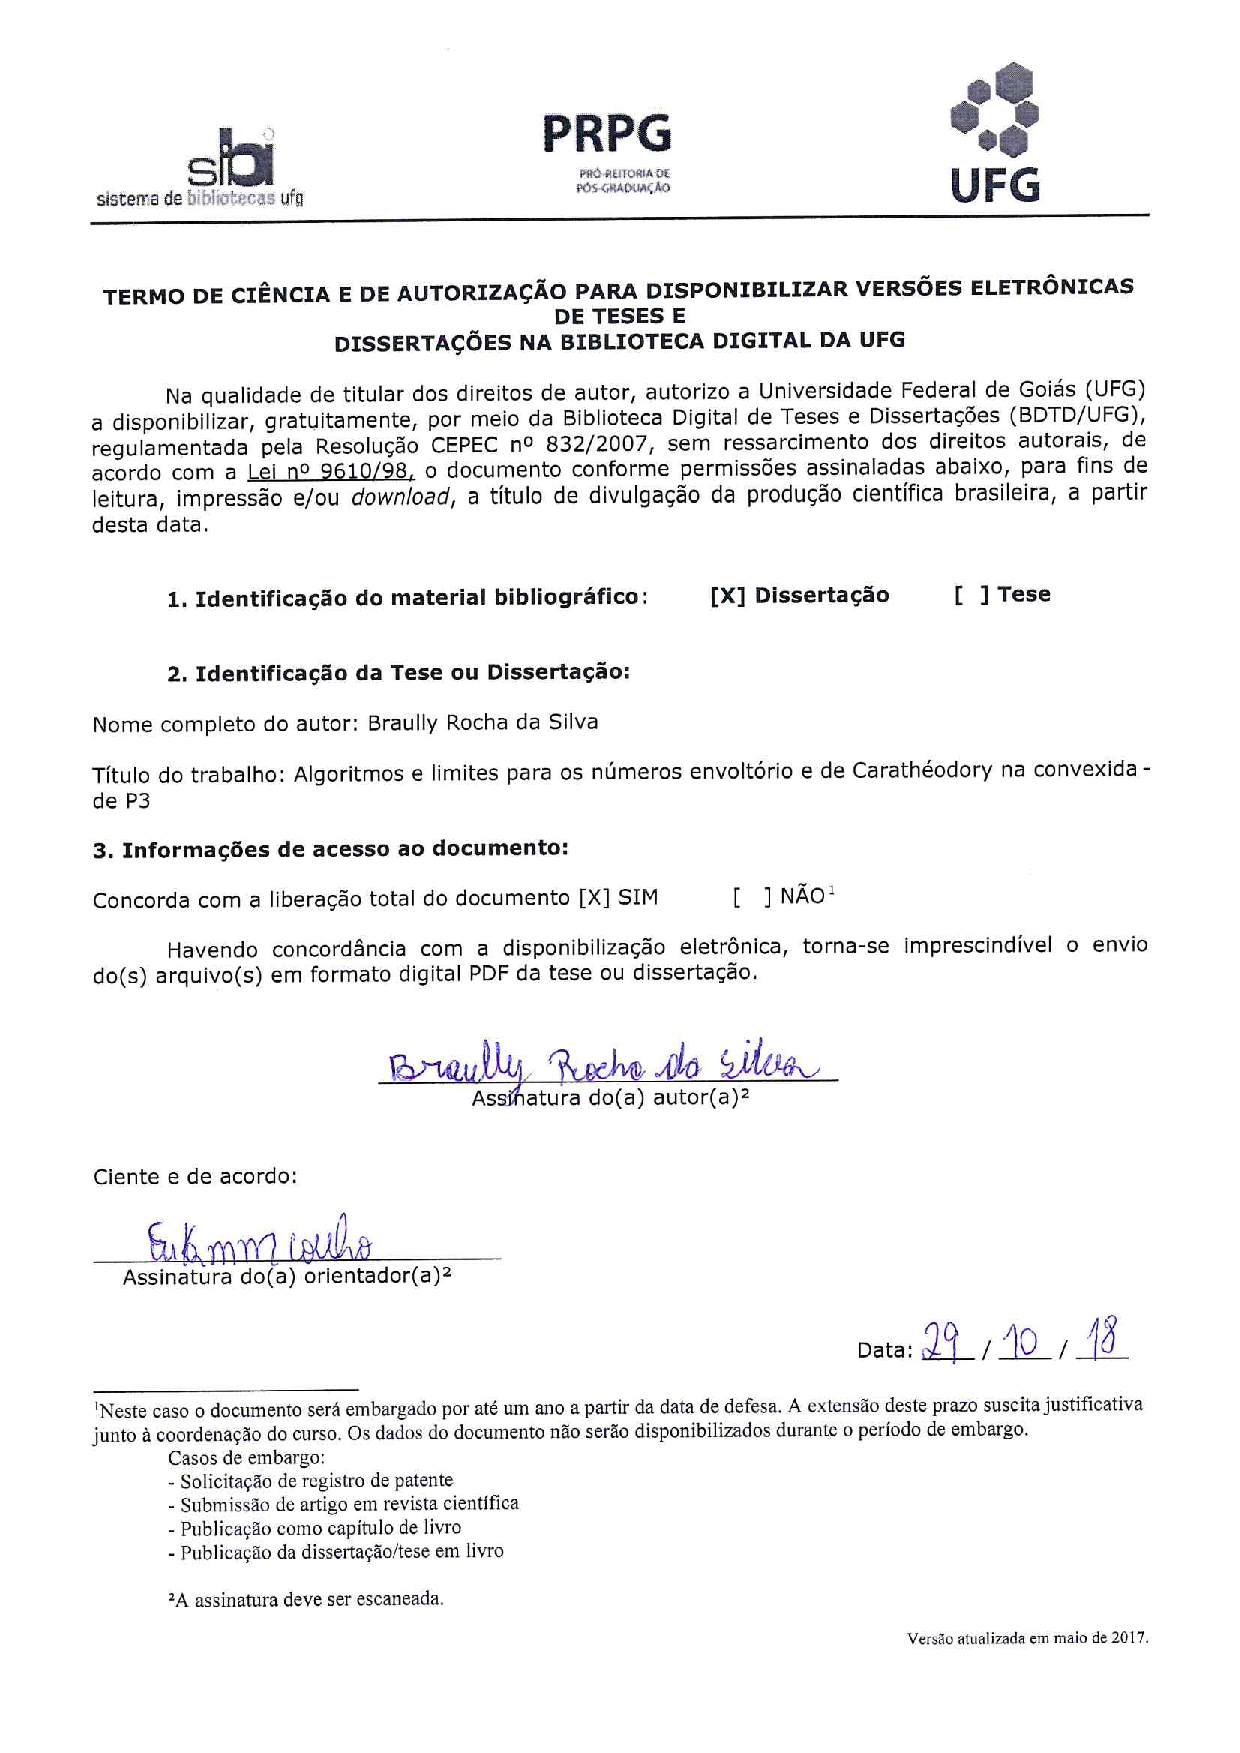
\includepdf[pages=-,pagecommand={},width=\textwidth]{imagens/doc00291520181029140039.pdf}
%\publica % Gera a autorização para publicação
\rosto   % Primeira folha interna do trabalho
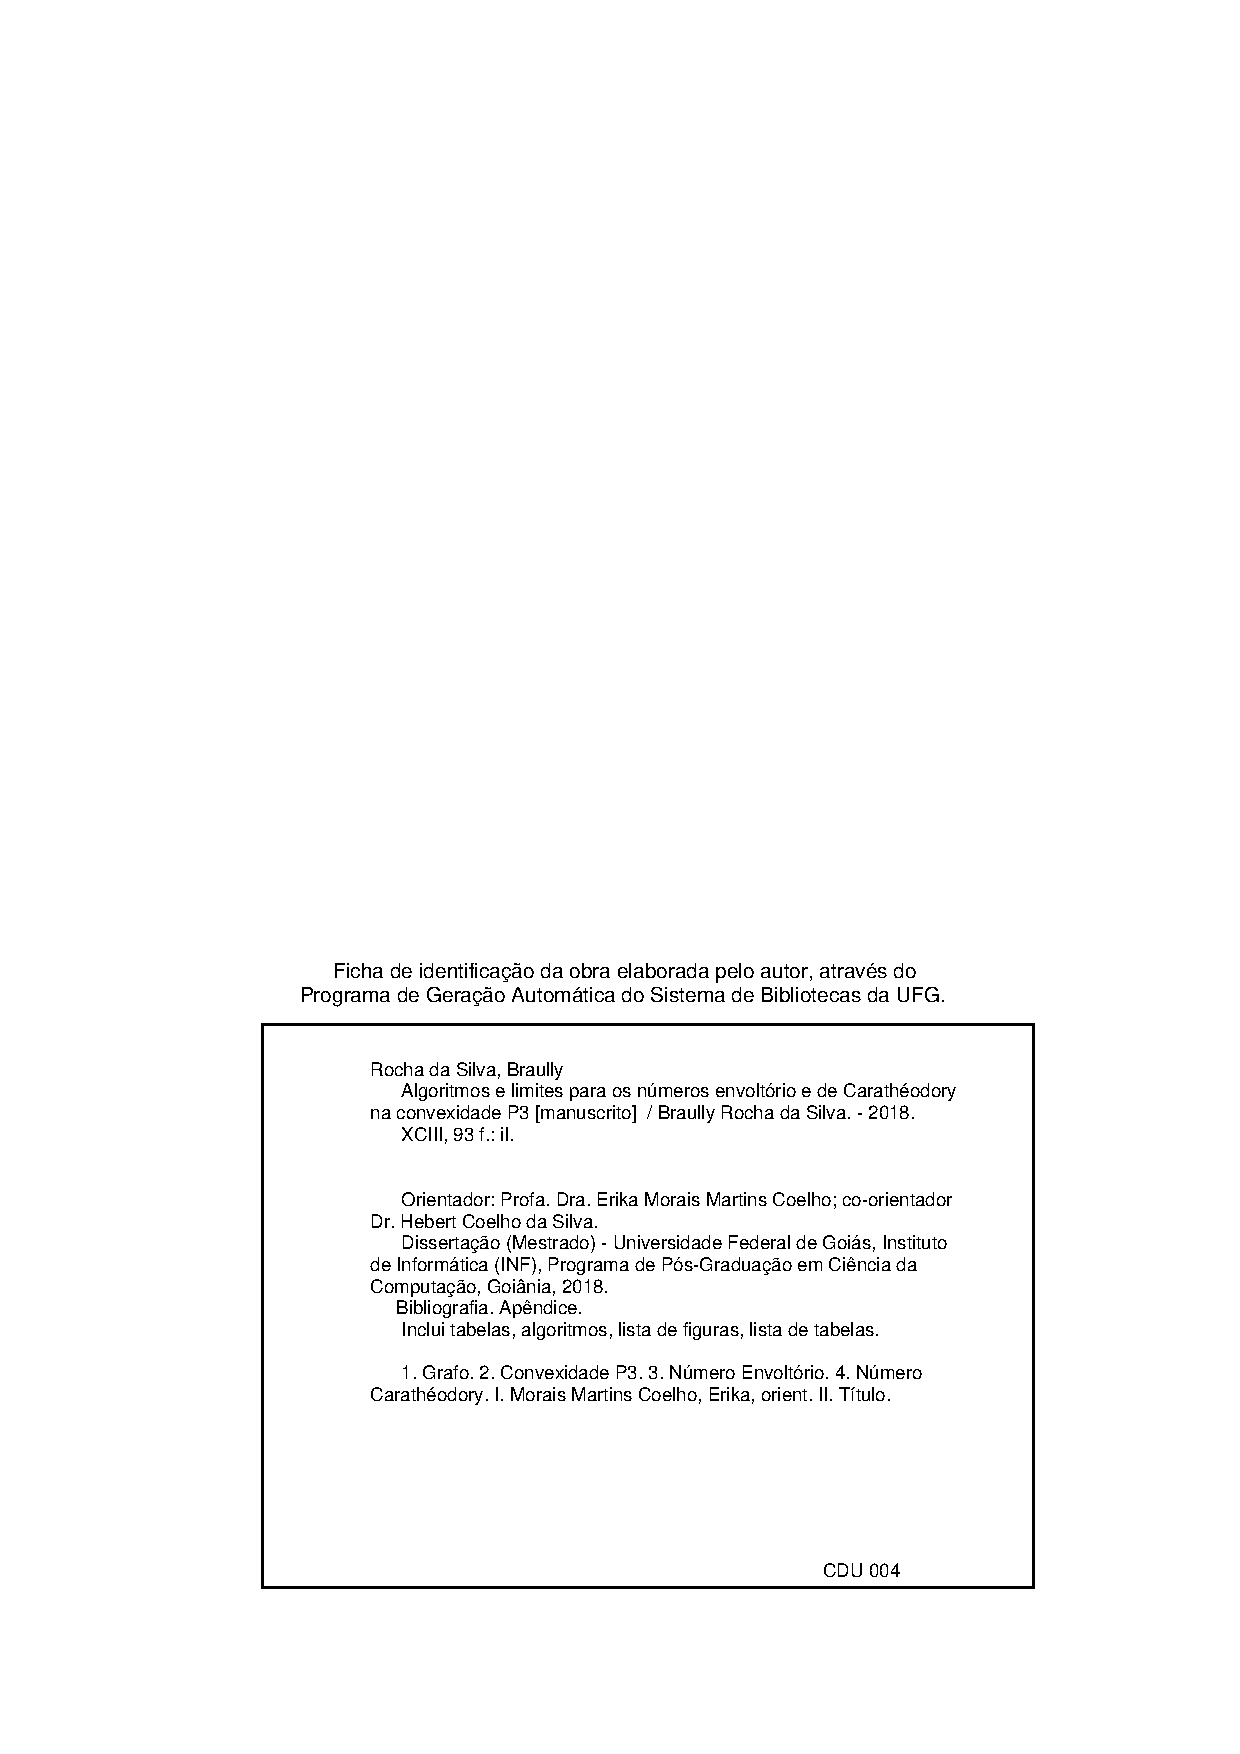
\includepdf[pages=-,pagecommand={},width=\textwidth]{imagens/ficha-catalografica.pdf}
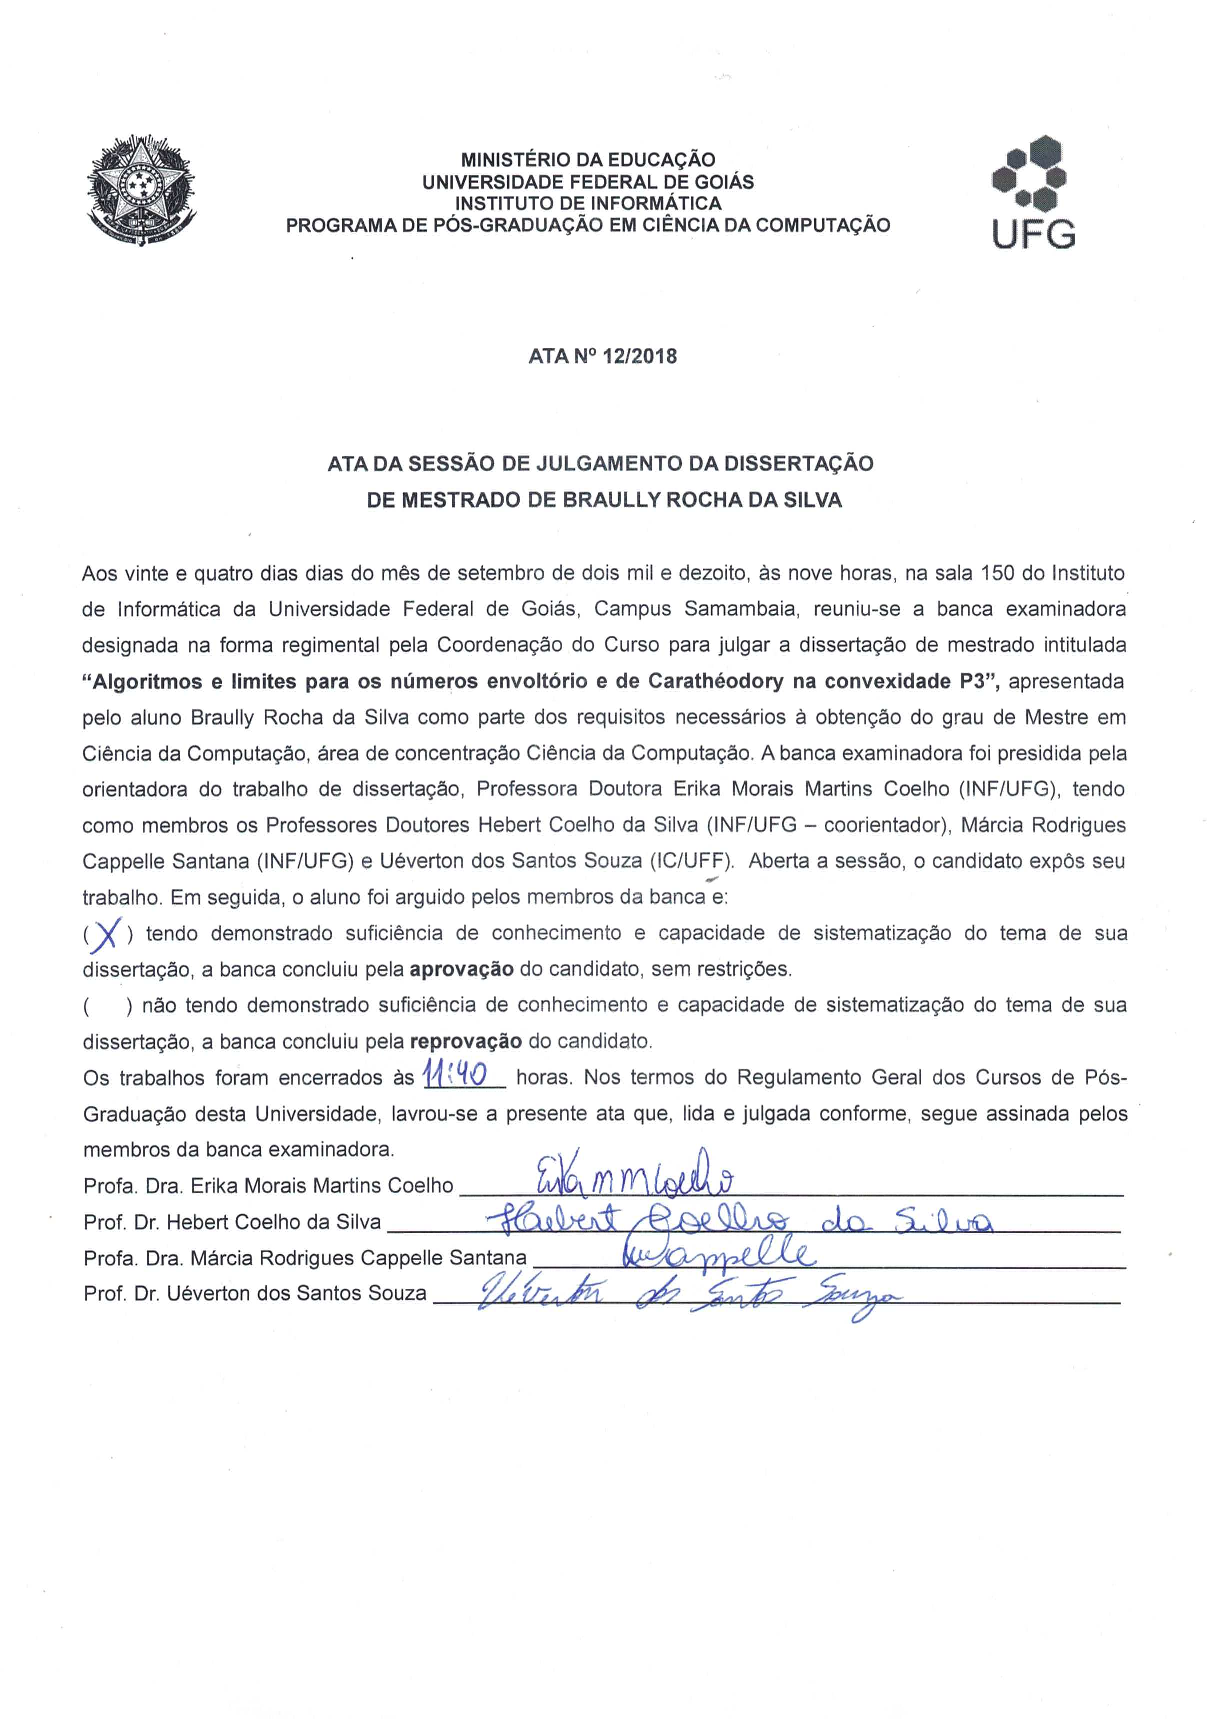
\includepdf[pages=-,pagecommand={},width=\textwidth]{imagens/BRN30055CB438A3_004905.pdf}
% \begin{aprovacao}
% \banca{Dra. Márcia Rodrigues Cappelle Santana}{Instituto de Informática\ -- UFG}
% \banca{Dr. Uéverton dos Santos Souza}{Instituto de Computação\ -- UFF}
% \end{aprovacao}

%\input{./pre/pre_aprovacao}
%\input{./pre/pre_direitos}
%\input{./pre/pre_dedicatoria}
%\input{./pre/pre_agradecimentos}
%\input{./pre/pre_epigrafe}
%\input{./pre/pre_resumo}
%\input{./pre/pre_abstract}

\chaves{Convexidade $P_3$, Número Envoltório, Número Carathéodory}
\begin{resumo} 
Nesta dissertação, tratamos de limites para o número envoltório e o número de Carathéodory na Convexidade $P_3$. Aferimos resultados para grafos de diâmetro 2 com vértice de corte para ambos os problemas. Adentrando em casos mais complexos, conseguimos determinar um limite logarítmico, por meio de algoritmo pseudo-polimonial, para o número envoltório de grafos de diâmetro 2 biconexos. Explorando um pouco mais restritivamente, conseguimos determinar um limite constante para algumas subclasses de grafos de diâmetro 2, os grafos maximais sem triângulo. Não atendo somente aos resultados teóricos, realizamos também implementações e algoritmos para esses parâmetros. As implementações perfazem algoritmos heurísticos, paralelos e força bruta. Por fim, embora não diretamente relacionado, desenvolvemos uma algoritmo para geração de grafos de Moore, que pode ser um dos caminhos para encontrar o ultimo grafo de Moore, caso ele exista. Questão que remanesce desconhecido e procurada por 55 anos. %E por fim concluímos com a exposição de algumas conjecturas que achamos interessantes, para supostos limites para o número envoltório e Carathéodory em outras classes de grafos, que não foram explorados neste trabalho, porém foi identificado pelas implementações, podendo ser melhor explorado em trabalhos futuros.
\end{resumo}

\keys{$P_3$ Convexity, Hull number, Carathéodory number}
\begin{abstract}{Algorithms and boundaries for hull and Carathéodory numbers in $P_3$ convexity}
In this work we present results and implementantions for hull and Carathéodory numbers in $P_3$ convexity. We obtain results for graphs of diameter 2 having cut-vertex for both problems. Finally, entering more complex cases, we were able to determine a logarithmic limit, means of algorithm, for the hull number in case of graph  diameter 2 and 2-connected. Exploring more restrictive cases, we determined a constant limit for some subclasses of graphs of diameter 2. We made also implementations and algorithms for these parameters. Implementations algorithms heuristic, parallel, and brute force. Finally, although not directly related, we developed an algorithm for Moore's graphs generation, which may be one of the ways to find Moore missinge graph, if it exists, a question that remains unknown for 55 years. And finally, we conclude with some conjectures interesting, for limits to the hull and Carathéodory numbers, in other classes of graphs, that were not explored in this work, but was identified by the implementations, and can be better explored in future works.
\end{abstract}
\tabelas[figtabalg]
%Opções:
%nada [] -> Gera apenas o sumário
%fig     -> Gera o sumário e a lista de figuras
%tab     -> Sumário e lista de tabelas
%alg     -> Sumário e lista de algoritmos
%cod     -> Sumário e lista de códigos de programas
% Pode-se usar qualquer combinação dessas opções.
% Por exemplo:
%  figtab       -> Sumário e listas de figuras e tabelas
%  figtabcod    -> Sumário e listas de figuras, tabelas e códigos de programas
%  figtabalg    -> Sumário e listas de figuras, tabelas e algoritmos
%  figtabalgcod -> Sumário e listas de figuras, tabelas, algoritmos e códigos de programas
%--------------------------------------------------------------- CAPÍTULOS %

\chapter{Introdução}
\label{cap:intro}

Um grafo sucintamente pode ser definido como um conjunto de elementos chamado de vértices, e por um conjunto de pares de vértices denominado arestas. Diversos problemas e relações do mundo real são modelados em grafos,
compondo uma ferramenta poderosa para o estudo e resolução de problemas. Embora vários problemas em grafos ainda sejam comprovadamente tidos como computacionalmente intratáveis (NP-Completo), como por exemplo, cacheiro viajante\cite{Biggs1986}, ainda assim são temas de interesse e ampla pesquisa. Em teoria dos grafos, como em outras disciplinas teóricas, alguns problemas são estudados e muitas vezes são resolvidos sem visar necessariamente a aplicação real e imediata. Na história da ciência moderna temos diversos exemplos, tais como a relatividade restrita e a mecânica quântica, que antes não tinham aplicações quando pesquisadas e hoje nos proporciona o gozar de tecnologias que vão do GPS à tomografia. Problemas como o Bóson de Higgs\cite{Higgs1964} foram estudados e resolvidos.Ainda permanecem sem aplicações práticas, porém cumprem seu papel preenchendo as lacunas na ciência.

Um caso interessante é o estudo da convexidade em grafos. Esse tópico foi motivado pelo estudo da convexidade geométrica na matemática. O início dos estudos nesta área data de aproximadamente 300 a.C
com os primeiros trabalhos de Euclides (300 a.C.) e seus polígonos convexos, mas somente a partir dos anos 30 se tem o início de estudos sistemáticos voltado á aplicações e convexidade de conjuntos.
Uma potencial e interessante aplicação do arcabouço teórico da convexidade
é o estudo do modelo de contaminação social ou disseminação de infecções \cite{Hodas2014}. Um indivíduo em uma rede se torna potencialmente contaminado a medida que seus vizinhos na rede ficam contaminados. Em publicação anterior \cite{Dreyer2009}, onde podemos ver um modelo matemático relativamente simples, baseado em grafos, que possibilita fomentar tais estudos. O modelo descreve os indivíduos por vértices e suas relações como arestas. Os vértices entram em um estado irreversível $X$ caso uma quantidade miníma $k$ de seus vizinhos também entrar nesse estado. Em \cite{Kuhlman2011} temos um estudo analítico e experimental de contaminação seguindo o modelo apresentado em \cite{Dreyer2009} limitado a 2 vizinhos. Esse modelo é compatível com os estudos de convexidade $P_3$ em grafos.

Na convexidade em grafos, podemos definir quando um subconjunto de vértices $S$ é um conjunto convexo. Na convexidade $P_3$ um subconjunto de vértices é convexo quando todo vértice tendo dois vizinhos em $S$, também estão em $S$. Dentro do universo de estudo de convexidades em grafos este trabalho realizou estudos e implementações pertinentes a dois parâmetros na convexidade $P_3$, a saber: número envoltório e número de Carathéodory na convexidade $P_3$.

O conceito do número envoltório foi introduzido por Everett e Seidman \cite{everett1985hull} na convexidade geodética e considera o conceito de envoltória convexa. Dado um conjunto $S$ de vértices, a envoltória convexa de $S$ é o menor conjunto convexo contendo $S$. E o número envoltório é a cardinalidade do menor conjunto $S$ tal que a envoltória convexa desse conjunto seja o conjunto de vértices do grafo. 
A determinação do número envoltório na convexidade $P_3$ é um problema NP-difícil, mas pode ser determinado em tempo polinomial para algumas classes, como cografos e grafos cordais \cite{Centeno}, e para prismas complementares \cite{duarte2015complexity}.

Recentemente, Penso Et. al\cite{Penso2015} estudaram a complexidade de calcular o número envoltório restrito a grafos planares com grau máximo limitado, mostrando que o problema continua NP-completo para grafos planares com grau máximo 3 e 4. Neste trabalho, estudamos o número envoltório considerando o diâmetro do grafo. Em particular, apresentamos um limite superior do número Envoltório $P_3$ para grafos de diâmetro 2 e também limites específicos para as subclasses maximal livre de triângulo e fortemente regulares. Os nossos resultados para grafos de diâmetro 2 e maximais livres de triângulo foram aceitos no Cologne-Twente Workshop on Graphs and Combinatorial Optimization 2018 - CTW 2018 e os limites para grafos fortemente regulares foram apresentados no VIII Latin American Workshop on Cliques in Graphs - LAWCG 2018 \cite{Coelho2018}.

Outro parâmetro bem conhecido sobre os conjuntos convexos é o número de Carathéodory. Este parâmetro surge do teorema de Carathéodory para conjuntos convexos no ${\cal R}^d$ \cite{Caratheodory1911}.
Com base neste teorema todo ponto $u$ na envoltória convexa de um conjunto $S \subseteq {\cal R}^d$ encontra-se no fecho
convexo de um subconjunto $F$ de $S$ de ordem no máximo $d+1$. Do teorema de Carathéodory surge  a definição do número de 
Carathéodory para grafos. Seja $G$ um grafo e ${\cal C}$ uma convexidade sobre V(G), o \textit{número de Carathéodory} c(G) é o menor inteiro c, para o qual todo $u \in H(S)$, existe um conjunto $F \subseteq  S$, com $|F| \le c$ e $u \in H(F)$.  Seja $G$ um grafo e $S$ um subconjunto de V(G). Se $\partial H(S)=H(S) \setminus \bigcup _{u \in S} H(S \setminus \{u\})$, é não vazio, então $S$ é um \textit{conjunto de Carathéodory}. Esta definição permite uma forma alternativa para o número de Carathéodory como sendo a maior cardinalidade de um conjunto de Carathéodory. Na convexidade $P_3$ a determinação do número de Carathéodory é um problema NP-completo, mesmo para grafos bipartidos cite{Barbosa2012}, mas possui determinação de tempo polinomial para árvores, grafos blocos \cite{Barbosa2012} e cordais \cite{Coelho2014}. Neste trabalho, consideramos o número de Carathéodory na convexidade $P_3$ para grafos de diâmetro 2 com vértice de corte e algumas subclasses dos grafos maximais livres de triângulo.

Ainda implementamos vários algoritmos. Desenvolvemos algoritmos de força bruta e algoritmo heurísticos para o número envoltório e número de Carathéodory. Como esses problemas são NP-completos, implementamos versões paralelas de todos eles com o objetivo de melhorar o tempo de execução. As implementações realizadas foram fundamentais para a escolha de trabalhar com grafos de diâmetro 2 e para as conjecturas levantadas e posteriormente provadas.

Com os algoritmos implementados desenvolvemos uma ferramenta simplificada, denominada {\it FATIG}, com facilidades para uso e novas implementações em outros tipos de problemas envolvendo grafos.

Por fim, tratamos dos grafos de Moore de diâmetro 2, 
que é um resultado colateral identificado ao longo deste trabalho. Os grafos de Moore são grafos de diâmetro 2 que atendem a igualdade que estabelecemos para os grafos maximais livre de triângulo. Foi desenvolvido um algoritmo capaz de gerar todos os três grafos de Moore, e este algoritmo pode ser uma ferramenta auxiliar para encontrar o último grafo de Moore. O último grafo de Moore, em suposição, é um grafo 57-regular com 3250 vértices. Sua existência ainda permanece um problema em aberto, mas vários de seus parâmetros e propriedades já foram identificados em outros trabalhos \cite{Godsil1995,Macaj2010,Miller2005}.

Este trabalho está dividido em 5 capítulos a saber: No capítulo \ref{cap-fundamentos} apresentamos os conceito básicos e notações utilizadas no trabalho, fazemos também uma revisão dos resultados conhecidos sobre o tema. No capítulo \ref{envoltoria} apresentamos nossos resultados sobre o número envoltório para grafos de diâmetro 2.
O capítulo \ref{cara} é dedicado aos resultados sobre o número de Carathéodory para alguns grafos de diâmetro 2.% sem $C_6$ com subgrafo induzido. 
 A discussão sobre os grafos de Moore estão no Capítulo \ref{moore} e as implementações dos algoritmos são apresentadas no Capítulo \ref{implementa}. Finalizamos o trabalho com nossas conclusões e propostas á futuros trabalhos.


\chapter{Preliminares}
\label{cap-fundamentos} 
\section{Fundamentos}
    Este capítulo nos traz alguns conceitos básicos relativos à teoria dos grafos e convexidade que serão necessários ao longo dos demais capítulos.
Os conceitos e notações relativos à teoria dos grafos e algoritmos
estão baseados nas referências \cite{Bondy1976,Cormen2002}. Assim como as  definições, teoremas e resultados de convexidade também estão baseados nas referências 
\cite{Balogh,Barbosa2012,Bollobas,CeciliaCenteno2012,Centeno,Coelho2014,Coelho2012,duarte2015complexity,Hon2016,De2016a,Penso2015,DraquePenso2014}.

\subsection{Grafos e Convexidade}
    
Um \textit{grafo simples} $G$ é definido por um conjunto finito e não vazio de vértices $V(G)$ e um conjunto de arestas $E(G)$, formado por pares não ordenados de elementos de $V(G)$. Neste trabalho utilizaremos grafos simples finitos, em que arestas não formam laço com o próprio vértice de origem e mais de uma aresta ligando o mesmo par de vértice.

Na Figura~\ref{fig:grafo-exemplo} temos um exemplo de um grafo simples, 
com um conjunto $V(G)$ de seis vértices $V(G) = \{1, 2, 3, 4, 5, 6\}$, 
e um conjunto $E(G)$ de nove arestas $E(G) = \{(1,2), (1,5), (2,3), (2,5), (3,4), (3,5), (3,6), (4,5), (4,6)\}$.
Nota-se que não existe mais de uma aresta ligando o mesmo par de vértices e nenhuma aresta formando um laço. 

\begin{figure}
\centering
\begin{tikzpicture}[scale=0.8,shorten >=1pt, auto, node distance=3cm, ultra thick,
node_style/.style={circle,draw=blue,fill=blue!20!,font=\sffamily\Large\bfseries},
node_style_selected/.style={circle,draw=black,fill=red!20!,font=\sffamily\Large\bfseries},
edge_style/.style={draw=black}]
\node[node_style] (v1) at (-2,2) {2};
\node[node_style] (v2) at (2,2) {3};
\node[node_style] (v3) at (4,0) {6};
\node[node_style] (v4) at (2,-2) {4};
\node[node_style] (v5) at (-2,-2) {5};
\node[node_style] (v6) at (-4,0) {1};
\draw[edge_style]  (v1) edge node{} (v2);
\draw[edge_style]  (v2) edge node{} (v3);
\draw[edge_style]  (v3) edge node{} (v4);
\draw[edge_style]  (v4) edge node{} (v5);
\draw[edge_style]  (v5) edge node{} (v6);
\draw[edge_style]  (v6) edge node{} (v1);
\draw[edge_style]  (v5) edge node{} (v1);
\draw[edge_style]  (v5) edge node{} (v2);
\draw[edge_style]  (v4) edge node{} (v2);
\end{tikzpicture}
\caption{Exemplo de um grafo}
\label{fig:grafo-exemplo}
\end{figure}


A \textit{vizinhança aberta} de um vértice consiste no conjunto de todos os seu vizinhos, e será denotada por: seja $v$ um vértice de $G$ então sua vizinhança aberta é $N_G(v)=N(v)=\{u \in V(G)|vu \in E(G)\}$. Ao passo que dado um conjunto qualquer de vértices a \textit{vizinhança aberta de um conjunto} é a união da vizinhança aberta de todos os seus elementos, denotada por $N_G(S)=N(S)=\{\forall v \in S| u \in N(S)|vu \in E(G)\}$.  A \textit{vizinhança fechada} é o conjunto formado pela vizinhança aberta do vértice união com ele próprio, será dada por $N_G[v] = N[v]=\{v\} \cup N_G(v)$. De maneira análoga  a \textit{vizinhança fechada de um conjunto}, consiste na união da vizinhança fechada de todos os seus elementos, denotada por $N_G[S]=N[S]=S\cup N(S)$.

Seja um grafo qualquer $G$, um \textit{subgrafo} de $G$ é um grafo $H$ cujo conjunto de vértices seja um subconjunto de $V(G)$ e o conjunto de arestas é um subconjunto de $E(G)$. Dado um subconjunto $S$ de vértices de $G$, podemos dizer que um \textit{subgrafo induzido}, é um subgrafo cujo conjunto de vértices é $S$, e o conjunto de arestas é o subconjunto de todas as arestas de $G$ que tenham as duas extremidades $S$. Dado um grafo $G$ e um vértice $v$ tal que $v \in V(G)$, para facilidades de notação, o subgrafo $G'$ induzido pelo conjunto de vértice $V(G)\setminus\{v\}$, será representado como $G'=G-v$.

Um \textit{caminho} em $G$ é uma sequência de vértices $P=v_0,v_1,\cdots,v_k$, tal que $v_iv_{i+1} \in E(G)$ para $i$ de $0$ até $k-1$. A \textit{distância} entre dois vértices é o comprimento do menor caminho entre eles. Sejam $u$ e $v$ dois vértices distintos de um grafo $G$. Vamos denotar a distância entre eles como $d_G(u,v)=d(u,v)$. E o \textit{diâmetro} de $G$ é a maior distância entre quaisquer dois vértices, será dado por $diam(G)=d$. 

Um grafo $G$ é dito \textit{conexo}, se para todo par de vértice existe um caminho de um para o outro. Caso contrário ele é tido como \textit{desconexo}. Em um grafo desconexo uma \textit{componente conexa} é formada por um conjunto de vértices que possuem caminho entre si, ou seja todos os vértices de uma componente conexa são acessíveis a outros vértices na mesma componente. O número de componentes conexas de $G$ será denotado por $\omega(G)$. Um grafo $G$ possui um \textit{vértice de corte} $c$ se o subgrafo $G'= G-c$ e tal que $\omega(G^\prime)>\omega(G)$. Por fim $G$ é dito \textit{biconexo} se é conexo e não possui vértice de corte. 

O \textit{grau}  de um vértice $v$ de $G$, será denotado como $d_G(v)=d(v)$ e é o número de arestas incidentes em $v$. O maior e menor graus dos vértices de $G$ serão respectivamente denotados por $\delta(G)$ e $\Delta(G)$. 

Um subconjunto $D \subseteq V(G)$ é um \textit{conjunto dominante} de $G$, se para todo $v \in V(G) \setminus D$, $v$ é adjacente a pelo menos um vértice de $D$. Um subconjunto $D \subseteq V(G)$ é um \textit{conjunto dominante total} de $G$, se para todo $v \in V(G)$, $v$ é adjacente a pelo menos um vértice de $D$.  A \textit{cintura} de um grafo $G$ é o menor ciclo de $G$. Um grafo $G((A,B),E)$ é dito \textit{bipartido} se seus vértices podem ser particionados em dois subconjuntos $A$ e $B$, de forma com que toda aresta de $G$ tem um extremo em $A$ e outro em $B$. $G$ é um grafo \textit{bipartido completo} se todo vértice em $A$ é adjacente a todo vértice em $B$. Por fim, $G$ é $k-$partido se os vértices de $G$ puderem ser particionados em $k$ subconjuntos, de forma que os vértices pertencentes a mesma partição não sejam adjacentes.

Um subconjunto $C_t \subseteq V(G)$ é um \textit{corte de vértices}, se a remoção de todos os vértices em $C_t$ desconecta $G$, de forma análoga com as arestas, um subconjunto $C_t \subseteq E(G)$ é um \textit{corte de arestas} se a remoção de todas as arestas desconecta $G$. Um \textit{corte mínimo} em um grafo é um subconjunto de vértices ou arestas, tal que não existe um subconjunto menor que é um \textit{corte de vértices} ou \textit{corte de arestas}, respectivamente.

Os grafos $G_1$ e $G_2$, são considerados \textit{isomorfos} se existe uma função $f$ bijetora tal que $f: V(G_1) \to V(G_2)$ e $u,v\in E(G_1)$ se somente se $f(u),f(v) \in E(G_2)$. Considerando essa relação como \textit{isomorfismo} temos o \textit{automorfismo} que é um isomorfismo de um grafo consigo mesmo, ou seja, em um grafo $G$ existem permutações de seus vértices, que são isomorfismos de $G$. Ainda no campo do \textit{automorfismo} para quaisquer dois pares de vértices de um grafo $G$, existe um automorfismo, então temos $G$ que é um grafo \textit{vértice-transitivo}, e se para qualquer dois pares de vértices a uma distância determinada, existe um automorfismo para qualquer outros dois pares de vértices a mesma distância, então $G$ é um grafo \textit{distância-transitivo}.


São tipos especiais de grafos, usados como exemplo mais a frente. O \textit{grafo estrela} é um grafo bipartido completo em que uma partição possui somente um vértice, em um \textit{grafo completo} todo par de vértice é adjacente entre si, um \textit{grafo caminho} consiste em um grafo conexo conexo, com dois ou mais vértices, que podem ser ordenados em um caminho passando por todos seus vértices, e por ultimo o \textit{grafo ciclo} que é um grafo que contem um único ciclo composto por todo os sues vértices. 


De modo geral, uma \textit{convexidade} em um grafo $G$ é dada por um conjunto ${\cal C}$, formado por subconjuntos de V(G) que atende as seguintes restrições:
\begin{itemize}
    \item[-] $\emptyset,V(G) \in {\cal C}$;
    \item[-] ${\cal C}$ é um conjunto fechado em relação a operação de interseção.
\end{itemize}
    Cada elemento de ${\cal C}$ é um \textit{conjunto convexo}
para uma convexidade ${\cal C}$. A \textit{envoltória convexa} $H_c(S)$ 
de um subconjunto $S$ é o menor conjunto convexo que contém S.
Um tipo de convexidade especial em grafos são as convexidades definidas através de um conjunto
${\cal P}$ de caminhos em grafos. Neste caso, um subconjunto ${\cal C} \in V(G)$ é convexo, principalmente
quando ${\cal C}$ contém todos os vértices pertencentes aos caminhos de ${\cal P}$ cujos vértices extremos estão também em ${\cal C}$. 

Podemos citar a \textit{convexidade geodésica},
definida no momento em que ${\cal P}$ é o conjunto de todos os caminhos mínimos de G, 
veja em \cite{Caceres2006,Dourado2016,Journal2010}, e também a \textit{convexidade $P_3$},
quando ${\cal P}$ é o conjunto de todos os caminhos com três vértices 
\cite{Barbosa2012,Centeno,Centeno2011,Coelho2014,Dourado2013}.

\subsection{Convexidade $P_3$}
\label{sec-convexidade-p3}
    De agora em diante iremos considerar ${\cal C}$ como convexidade $P_3$.
Como um grafo $G$ unicamente determina sua convexidade $P_3$ utilizaremos
$H(S)$ ao invés de $H_c(S)$.

Dado um subconjunto $S \subseteq V(G)$, o \textit{intervalo fechado} 
$I{[}S{]}$ de $S$ é formado por $S$ simultaneamente com todo vértice de $V(G) \setminus S$
com pelo menos dois vizinhos em $S$. Se $I{[}S{]}=S$ então $S$ é um conjunto convexo.
Podemos utilizar o intervalo fechado para iterativamente calcular a envoltória convexa de 
um subconjunto $S \subseteq V(G)$. Assim a envoltória convexa pode ser formada
por uma sequência $I^p[S]$ onde $p$ é um inteiro não negativo,  
$I^0{[}S{]}=S$, $I^1{[}S{]}=I{[}S{]}$ e $I^p{[}S{]}=I[I^{p-1}]$ para $p \ge 2$.
Quando para algum $p$, temos $I^q{[}S{]} = I^p{[}S{]}$, para todo $q \ge p$, temos
então $I^p{[}S{]}$, considerando-o  um conjunto convexo.

Considere o grafo $G$ na Figura~\ref{fig:grafo-petersen} e o subconjunto $S_0 = \{4, 5, 8, 9\}$ de V(G). O Conjunto $S_0$ não é um conjunto convexo, por exemplo, existe o caminho $P=5,7,9$ em que os vértices $5$ e $9$ então no conjunto e o vértice $7$, vizinho a $5$ e $9$, não está. Já que o conjunto não é convexo, qual seria o menor conjunto convexo que contém $S_0$?
Para responder essa pergunta, precisamos calcular a envoltória convexa de $S_0$, 
tal como se segue:

Vamos computar a envoltória convexa do conjunto $S_0$:
\begin{itemize}
    \item{$I^1{[}S_0{]}=\{0, 3, 4, 5, 6, 7, 8, 9\}$}
    \item{$I^2{[}S_0{]}=I{[}I^1{[}S_0{]}{]}=\{0, 1, 2, 3, 4, 5, 6, 7, 8, 9\}$}
    \item{$I^3{[}S_0{]}=I{[}I^2{[}S_0{]}{]}=I^2{[}S_0{]}=\{0, 1, 2, 3, 4, 5, 6, 7, 8, 9\}$}
\end{itemize}

    Com isso determinamos o menor conjunto convexo para o grafo do exemplo 
que contém o conjunto $S_0$. Logo $H(S_0)=\{0, 1, 2, 3, 4, 5, 6, 7, 8, 9\}$.

\begin{figure}
\centering
\begin{tikzpicture}[scale=0.8,shorten >=1pt, auto, node distance=3cm,
node_style/.style={circle,draw=blue,fill=blue!20!,inner sep=0pt, minimum width=4pt,font=\sffamily\small},
node_style_selected/.style={circle,draw=black,fill=red!20!,font=\sffamily\Large\bfseries},
edge_style/.style={draw=black}]
\node[node_style] (v0) at (0,3.5) {0};
\node[node_style] (v1) at (3,1.5) {1};
\node[node_style] (v2) at (2,-2) {2};
\node[node_style] (v3) at (-2,-2) {3};
\node[node_style] (v4) at (-3,1.5) {4};
\node[node_style] (v5) at (0,2) {5};
\node[node_style] (v6) at (1.5,1) {6};
\node[node_style] (v7) at (1,-1) {7};
\node[node_style] (v8) at (-1,-1) {8};
\node[node_style] (v9) at (-1.5,1) {9};

\draw[edge_style]  (v0) edge node{} (v1);
\draw[edge_style]  (v0) edge node{} (v4);
\draw[edge_style]  (v0) edge node{} (v5);
\draw[edge_style]  (v1) edge node{} (v2);
\draw[edge_style]  (v1) edge node{} (v2);
\draw[edge_style]  (v1) edge node{} (v6);
\draw[edge_style]  (v2) edge node{} (v3);
\draw[edge_style]  (v2) edge node{} (v7);
\draw[edge_style]  (v3) edge node{} (v4);
\draw[edge_style]  (v3) edge node{} (v8);
\draw[edge_style]  (v4) edge node{} (v9);
\draw[edge_style]  (v5) edge node{} (v7);
\draw[edge_style]  (v5) edge node{} (v8);
\draw[edge_style]  (v6) edge node{} (v8);
\draw[edge_style]  (v6) edge node{} (v9);
\draw[edge_style]  (v7) edge node{} (v9);
\end{tikzpicture}
\caption{Grafo de Petersen, $G_{pn}$}
\label{fig:grafo-petersen}
\end{figure}

Se $H(S)=V(G)$ dizemos que $S$ é  um \textit{conjunto de envoltória}, ou conjunto envoltório. 
A cardinalidade $h(G)$ do menor conjunto de envoltória em $G$ é chamado de 
\textit{número envoltório}.

Apesar da aparente simplicidade proveniente da definição,
os estudos em \cite{Dourado2009} permitem inferir que determinar o número envoltório para grafos gerais é um prolema NP-Completo.

No exemplo da Figura~\ref{fig:grafo-petersen} 
temos a envoltória convexa do conjunto $S_0$ que é equivalente ao conjunto de vértices.
Nesse caso, temos que $S_0$ é um conjunto de envoltória, porém, existem conjuntos de envoltória de cardinalidade menor que $S_0$,
como por exemplo $S_1=\{4,7,8\}$. Como não existe nenhum conjunto de envoltória de cardinalidade 2, concluímos que h(G)=3.


Um resultado habitual sobre os conjuntos convexos no ${\cal R}^d$ é o teorema de Carathéodory \cite{Caratheodory1911}.
Este teorema afirma que todo ponto $u$ na envoltória convexa de um conjunto $S \subseteq {\cal R}^d$ encontra-se no fecho
convexo de um subconjunto $F$ de $S$ de ordem no máximo $d+1$. Do teorema de Carathéodory surge  a definição do número de 
Carathéodory para grafos. Seja $G$ um grafo e ${\cal C}$ uma convexidade sobre V(G).
O \textit{número de Carathéodory} c(G) é o menor inteiro c,
para o qual todo $u \in H(S)$, existe um conjunto $F \subseteq  S$,
com $|F| \le c$ e $u \in H(F)$. 

Seja $G$ um grafo e $S$ um subconjunto de V(G). Se $\partial H(S)=H(S) \setminus \bigcup _{u \in S} H(S \setminus \{u\})$,
é não vazio, então $S$ é um \textit{conjunto de Carathéodory}. Esta definição permite um sistema alternativa,
o número de Carathéodory como sendo a maior cardinalidade de um conjunto de Carathéodory. 

Considere o grafo $G$ da Figura~\ref{fig:grafo-petersen}. Observe que $S_1=\{4,7,8\}$ é um conjunto de 
Carathéodory, porém, existem conjuntos de Carathéodory de cardinalidade maior que $S_1$, como por exemplo o
próprio conjunto $S_0 = \{4,5,8,9\}$. Note que $H(S_0)=\{0, 1, 2, 3, 4, 5, 6, 7, 8, 9\}$.
Neste momento aplicando a definição do conjunto de Carathéodory iremos determinar o $\partial H(S_0)$:
\begin{itemize}
    \item{Conforme já determinado anteriormente, $H(S_0)=\{0, 1, 2, 3, 4, 5, 6, 7, 8, 9\}$}
    \item{Aplicando a envoltória convexa, temos $H(S_0 \setminus \{4\})=\{5,8,9,6,7\}$}
    \item{Aplicando a envoltória convexa, temos $H(S_0 \setminus \{5\})=\{4,8,9,3,6\}$}
    \item{Aplicando a envoltória convexa, temos $H(S_0 \setminus \{8\})=\{4,5,9,0,7\}$}
    \item{Aplicando a envoltória convexa, temos $H(S_0 \setminus \{9\})=\{4,5,8,0,3\}$}
    %\item{Aplicando a envoltória convexa, temos $H(S_0 \setminus \{9\})=\{4,5,8,0,3\}$}
    \item{$\partial H(S_0)=H(S_0) \setminus (H(S_0 \setminus \{4\}) \cup H(S_0 \setminus \{5\}) \cup H(S_0 \setminus \{8\}) \cup H(S_0 \setminus \{9\}))$}
    \item{Com os resultados anteriores podemos obter a informação de que: $\partial H(S_0)=\{1,2\}$}
\end{itemize}

Como o conjunto $\partial H(S_0)$ não é vazio, 
podemos concluir que $S_0$ é um conjunto de Carathéodory.
Dado que não existem conjuntos de Carathéodory 
de cardinalidade maior do que quatro,
alimentamos que esse é o número de Carathéodory do grafo $G$,
isto é, $c(G_{pn})=4$.

Em \cite{Barbosa2012} demonstra-se que determinar o Número de Carathéodory na Convexidade $P_3$
é um problema NP-Completo mesmo para grafos bipartidos. 
Podemos inferir assim, a dificuldade na definição de tal parâmetro para grafos gerais. 
Embora o problema seja NP-Completo, 
para algumas classes foi possível definir um limite máximo 
ou um algoritmo polinomial que determine esse parâmetro,
tais como árvores e blocos \cite{Coelho2012}. 


\subsection{Algoritmos e Classe de Complexidade}

Três classes de problema são bem conhecidas na literatura: P, NP e NP-Completo. 
A classe P trata-se da classe dos problemas com solução polinomial, isto é, problemas que admitem algoritmos em tempo $O(n^c)$ em que $c$ é uma constante e $n$ o tamanho da entrada.
São na prática, problemas tido como tratáveis. A segunda classe, 
os problemas NP, são os problemas cujo certificado da solução pode ser verificado em tempo polinomial.

Por fim, temos a classe de problemas NP-Completo,
que consistem em problemas NP e cuja complexidade 
é igual ou superior aos problemas mais difíceis em NP.
Até o momento, não é conhecido solução polinomial para qualquer problema dessa classe. Por isso os problemas nessa classe, são tidos na prática como 
computacionalmente intratáveis.

Uma interessante subclasse dos problemas NP-Completo,
são os Pseudo-polinomiais ou Quasi-polinomiais.
Diz respeito a problemas que para determinadas instâncias de problemas
tem complexidade polinomial para determinados parâmetros da entrada.
Por exemplo, sabemos que é um problema NP-Completo determinar se um grafo $G$, com $n$ vértices, tem um conjunto envoltório de tamanho $k$. Mas, se para certas classes de grafos, for possível encontrar um conjunto envoltório em tempo polinomial, quando $k$ maior que uma função determinada $k>f(n)$, podemos dizer que o número envoltório é um problema pseudo-polinomial quando restrito as classes específicas.


%Nesse caso temos que como entrada do problema o grafo e a constante $k$, mas podemos determinar que para certas classes de grafos, se conseguirmos determinar que é possível encontrar um conjunto envoltório em tempo polinomial, quando for $k$ maior que uma função determinada $k>f(n)$, podemos dizer que o número envoltório é um problema pseudo-polinomial nesses casos. 

%Os problemas NP-Completos remanescem na literatura como intratáveis.
%Até o momento não foi possível demonstrar que admitem solução polinomial
%ou mesmo que é impossível.

Segundo \cite{Cormen2002} muitos problemas NP-Completos,
apesar de intratáveis, são relevantes demais para não se tentar uma solução. 
De acordo com \cite{Cormen2002} há três possíveis caminhos:
1) O isolamento de casos específicos e que possam ser resolvidos polinomialmente;
2) Um algoritmo exponencial para entradas relativamente pequenas;
3) Algoritmos heurísticos que produzam soluções quase ótimas.

Neste trabalho, exploramos um pouco de cada um desses caminhos
para obter um conjunto de soluções capazes de auxiliar 
nos estudos dos parâmetros de convexidade $P_3$.

Existem casos polinomiais identificados na literatura
que foram listados na revisão bibliográfica. 
No resultado das execuções outros possíveis casos foram identificados
e serão mencionados no que se refere aos resultados obtidos.

Para que entradas mais avançadas pudessem ser analisadas
os algoritmos exponenciais foram implementadas em duas versões, uma sequencial e outra paralela. 
Na implementação paralela foi utilizada a arquitetura CUDA,
que é baseada nas Unidades de Processamento Gráfico (GPU) da NVIDIA.
Pois ela nos permite o uso deste poder de processamento de baixo custo para computação de propósito geral.

A programação paralela eficiente traz vários desafios ausentes na programação tradicional, 
tais como: - equilibrar de maneira mais igualitária possível o trabalho das \textit{threads}, - utilizar o mínimo necessário de acesso a memória global e a sincronização de \textit{threads}, -uniformizar o acesso aos dados de trabalho das \textit{threads} o máximo possível,
dentre outros, sob pena da solução paralela ser mais ineficiente do que a solução sequencial.

Os algoritmos heurísticos foram concebidos a partir de uma abordagem gulosa,
onde em cada etapa a melhor solução é escolhida localmente na 
tentativa de maximizar ou minimizar o resultado final. 
Apesar de ser uma abordagem simples para tratar de um problema NP-Completo,
apresentou bons resultados para alguns tipos de grafos.

%/* Explicação breve sobre complexidade de algoritmo, força bruto e algoritmos aproximativos */


\section{Grafos de diâmetro 2}

Um grafo $G$ é dito de diâmetro 2 se a maior distância entre quaisquer dois vértices é 2. Em outras palavras, $G$  não é completo e todo par de vértices $u,v \in V(G)| (u,v) \in E(G)$ ou $N(u) \cap N(v) \ne \emptyset$. A classe de grafos de diâmetro 2 é ampla e inclui duas classes de interesse desse trabalho: é fortemente Regular conexos e Maximais Sem triângulo, cujo as definições já foram apresentadas anteriormente.

Apesar de serem classes distintas, existem alguns grafos fortemente regulares que também são maximais sem triângulo.  Esses grafos são também conhecidos como \textit{fortemente regulares sem triângulo}, que podemos ver na Figura~\ref{figconjts}. Na literatura atual são conhecidos apenas sete: $C_5$, grafo de Petersen, Clebsch, Hoffman-Singleton, Gewirtz e Higman-Sims. Ainda subsiste desconhecido um oitavo grafo de diâmetro 2 e fortemente regular, que caso venha se confirmar poderemos dizer que é um grafo de Moore 57-regular, contendo 3250 vértices e cintura 5 \cite{Godsil1995}.

\begin{figure}[h]
    \centering
    \begin{tikzpicture}
    \draw  (-2,2) ellipse (1.5 and 2);
    \draw  (0,2) ellipse (1.5 and 2);
    \draw  (-1,2) ellipse (3 and 3.5);
    \node at (-1,2) {FRST};
    \node at (-1,6) {Grafos 2-diâmetro};
    \node at (-2.3,2) {FR*};
    \node at (0.3,2) {MST};
    \end{tikzpicture}
    \caption{Grafos de 2-diâmetro, Fortemente Regular Conexos (FR*), Maximais Sem Triângulo (MST) e Fortemente Regulares Sem Triângulo (FRST)}
    \label{figconjts}
\end{figure}

\subsection{Maximal Sem Triângulo}
\label{sec-mst}
Um grafo $G$ é \textit{maximal sem triângulo} se a adição de qualquer aresta em $G$
formar um triângulo. Um grafo $G$ é dito \textit{diâmetro 2-crítico} ou \textit{diâmetro 2 minimal}  se ele tem diâmetro 2 e a remoção de qualquer aresta implica em um aumento do diâmetro do grafo. Em outras palavras $G$ é \textit{diâmetro 2-crítico} se $d(G)=2$ e $\forall e\in E(G) \Rightarrow d(G-e)>2$.  Em \cite{Mathematics1995,Barefoot1995} temos a demonstração  de que todo grafo maximal sem triângulo é um grafo de diâmetro 2 minimal, cuja deleção de qualquer aresta aumentaria o diâmetro do grafo. Enquanto para \cite{Brandt2000} todo grafo com pelo menos 3 vértices e diâmetro 2 é um grafo livre de triângulo. Exemplos: grafo estrela, completo bipartido e grafo de Petersen. 


 %Theorem 1: A triangle-free Graph is MTF if and only if it is MD2. [BAREFOOT199593]
%Não econtrei definição melhor em artios em inglês é referenciado como "diameter 2-critical graphs",
% porém não encontrei nenhum bom artigo em português que os cite


\subsection{Fortemente regular}
\label{sec-fr}

Um grafo $G$ é \textit{fortemente regular} se for um grafo k-regular 
e existir dois inteiros $b$ e $c$ tais que todos dois vértices adjacentes têm $b$ vizinhos em comum e todos dois vértices não adjacentes têm $c$ vizinhos em comum, podendo ser definido pelos parâmetros $(n,k,b,c)$. Tais como exemplos, temos alguns grafos bastante conhecidos e seus respectivos parâmetros listados na Tabela~\ref{tab-exemplos-grafos-fr}.
%Octahedral (6,4,2,4), $C_5$ (5,2,0,1), Hoffman-Singleton (50,7,0,1), Gewirtz (56,10,0,2) e Berlekamp-van Lint-Seidel (243,22,1,2). Se o parâmetro $c=0$ então o grafo é desconexo ou completo, pois todo par de vértice não é adjacente ou não possui vizinhos em comum. Os grafos fortemente regulares desconexos não são objeto de estudo deste trabalho.

\begin{table}[h]
\centering
\caption{Exemplos de grafos e parâmetros}
\label{tab-exemplos-grafos-fr}
\begin{tabular}{|l|l|}
\hline
\textbf{Grafo}            & \textbf{Parâmetro} \\ \hline
Octahedral                & (6,4,2,4)          \\ \hline
$C_5$                     & (5,2,0,1)          \\ \hline
Hoffman-Singleton         & (50,7,0,1)         \\ \hline
Gewirtz                   & (56,10,0,2)        \\ \hline
Berlekamp-van Lint-Seidel & (243,22,1,2)       \\ \hline
\end{tabular}
\end{table}

%/* Aparentemente é um probLema em aberto na literatura a quantidade desses grafos,
% 7  sãoconhecidos: http://www.math.ru.nl/OpenGraphProblems/Tjapko/30.html 
%Artigo Norman Brigs (não publicado): https://arxiv.org/pdf/0911.2160.pdf %http://www.maths.lse.ac.uk/Personal/norman/SRNT.pdf
%*/



\subsection{Propriedades dos Grafos de diâmetro 2}

Os grafos de diâmetro 2 possuem importantes propriedades. Podemos citar a cintura $g$ que é $3 \le g \le 5$, ou infinita quando é uma estrela \cite{Desormeaux2013}. Outra propriedade importante é que para qualquer $v \in V(G)$ o conjunto $N(v)$ é um conjunto dominante, ou seja, o conjunto formado pelos vizinhos de qualquer vértice é um conjunto dominante, conforme ilustrado na Figura~\ref{fig:tds}.

\begin{figure}
\centering
\begin{tikzpicture}
    \draw  (0,0) ellipse (1 and 2);
    \node[circle,draw,label=$v$] (v1) at (-1.5,0) {};
    \node[circle,draw,label=$n_{1}$] (v2) at (0,1) {};
    \node[circle,draw,label=below:$n_{k}$] (v3) at (0,-1) {};
    \draw [very thick,dotted] (0,0.3) -- (0,-0.3);

    \node (v7) at (0,0) {};

    \draw  (v1) edge (v2);
    \draw  (v1) edge (v3);

    \node at (0,2.5) {$N(v)$};

    \draw  (2.5,0) ellipse (1 and 2);
    \node at (2.5,2.5) {$V(G) \setminus N(v)$};

    \node[circle,draw,label=$u_1$] (v4) at (2.5,1) {};
    \node (v5) at (2.5,0) {};
    \draw [very thick,dotted] (2.5,0.3) -- (2.5,-0.3);
    \node[circle,draw,label=below:$u_x$] (v6) at (2.5,-1) {};

    \draw  (v2) edge (v5);
    \draw  (v2) edge (v4);
    \draw  (v3) edge (v6);
    \draw  (v3) edge (v5);
    \draw  (v7) edge (v5);
\end{tikzpicture}
\caption{$\forall v \in V(G)$  $N(v)$ é um conjunto dominante}
\label{fig:tds}
\end{figure}

\begin{proposition} Seja G um grafo de diâmetro 2.
\begin{enumerate}[label=(\alph*)] % (a), (b), (c), ...
   \label{prop:diametro2}
    \item{Para todo $u,v \in V(G)$, $u$ e $v$ são adjacentes ou tem um vizinho em comum} \label{pro-diam-2-itema}
    \item{$N(v)$ é um conjunto dominante $\forall v \in V(G)$} \label{pro-diam-2-itemb}
    \item{Se $\delta(G)=1$ então $\Delta(G)=n-1$}
    \item Se $v \in V(G)$ é um vértice de corte então $d(v)=n-1$\label{pro-diam-2-itemd}
    \item{Se $G$ tem vértice de corte então $\Delta(G)=n-1$}\label{pro-diam-2-iteme}
    \item Existe no máximo um vértice de corte em $G$\label{pro-diam-2-itemf}
    \item{Se $v_1,v_2 \in V(G)$ então $N[v_1] \cap N[v_2] \ne \emptyset$}
\end{enumerate}
\end{proposition}
\begin{proof}

Se $G$ tem diâmetro 2, então qualquer vértice $u$ tem um caminho até outro vértice $v$ passando por no máximo 2 arestas. Desta forma todo par de vértice em $G$ é adjacente ou possuem um vértice em comum, podemos assim concluir a proposição ~\ref{prop:diametro2}(a).

$N(v)$ é um conjunto dominante. Seja $u$ e $v$, dois vértices não adjacentes, supomos por contradição que não existe aresta de $u$ param $N(v)$, então não existe caminho $vwu$ visto que $w\in N(v)$, dessa forma a menor distância de $u,v$ é maior do que dois o que é uma contradição, pois $G$ tem diâmetro 2. Dessa forma podemos concluir a proposição ~\ref{prop:diametro2}(b).

Se $\delta(G)=1$ então $\exists v \in V(G)|d(v)=1$. Pela proposição anterior $N(v)$ é um conjunto dominante, como $v$ possui um único vizinho $u$, então $u$ é adjacente a todos os vértices $V(G)\setminus \{u\}$, e $d(u)=|V(G)|-1=n-1$. Com isso temos provado a proposição ~\ref{prop:diametro2}(c).

Se $G$ possui um vértice de corte $c$ e $\omega(G-c)$ o número de componentes conexas de $G-c$, então $\omega(G-c)>1$. Seja $C_x$ as componentes conexas do grafo $G-c$, supomos por contradição que $d(c)<n-1$, então existe um vértice $v \in C_i$, que não é adjacente a $c$ e nenhum vértice em $C_j$, tal que $i\neq j$. Porém, como $G$ tem diâmetro 2 então $\forall u \in C_j$, existe um caminho $uwv$ tal que $w\ne c$, dessa forma $v$ é adjacente a todos os vértices de $C_j$, o que consideramos uma contradição, pois, estão em componentes conexas distintas. Isso prova ~\ref{prop:diametro2}(d).

Se $G$ possui um vértice de corte, pela Proposição~\ref{pro-diam-2-itemd}, existe um vértice $v$ tal que $d(v)=n-1$. Por $G$ ser um grafo simples então não existe vértice $u\in V(G)$ tal que $d(u)>d(v)=n-1$. Portanto, concluímos que $\Delta (G) = n-1$. Isso prova ~\ref{prop:diametro2}(e).

Supomos por contradição que $G$ possui dois ou mais vértices de corte, $v_1,v_2,...,v_k$. Pela Proposição~\ref{pro-diam-2-itemd} sabemos que esses vértices são adjacentes a todos os demais vértices de $G$, então temos o grafo $G-v_1$ que possui duas ou mais componentes conexas. Em uma das componentes conexas teremos $v_2$ que também é um vértice de corte, em outra componente conexa distinta teremos $v_c$, por $v_2$ ser um vértice de corte é adjacente a todos os demais vértices inclusive $v_c$. Portanto, deveriam estar na mesma componente conexa, o que é uma contradição, pois, $v_c$ pertence a uma componente conexa diferente de $v_2$, logo, concluímos que $\Delta (G) = n-1$, o que prova ~\ref{prop:diametro2}(f).

Seja $G$ um grafo de diâmetro 2 e vértices $v_1,v_2 \in V(G)$ então $N[v_1] \cap N[v_2] \ne \emptyset$. Se $v_1$ e $v_2$ são adjacentes então $\{v_1, v_2\} \subseteq N[v_1] \cap N[v_2]$. Se $v_1$ e $v_2$ não são adjacentes, então por definição $\exists n_1 \in V(G)$ tal que $n_1 \in N(v_1) \cap N(v_2)$, o que implica na proposição ~\ref{prop:diametro2}(g) e que pode ser visto na Figura~\ref{fig:setunion}.
\end{proof}

\begin{figure}[h]
\centering
\begin{tikzpicture}
  \draw  (-2,1.5) ellipse (3.5 and 1.5);
  \draw  (2,1.5) ellipse (3.5 and 1.5);
  \node at (0,1.5) {$N[v_1] \cap N[v_2]$};
  \node at (-3,1.5) {$N[v_1] \setminus N[v_2]$};
  \node at (3,1.5) {$N[v_2] \setminus N[v_1]$};
  
  \node at (-2,3.5) {$N[v_1]$};
  \node at (2,3.5) {$N[v_2]$};
\end{tikzpicture}
\caption{$N[v_1]$ e $N[v_2]$, relação entre a vizinhança fechada de qualquer 2 vértices em um grafo de diâmetro 2}
\label{fig:setunion}
\end{figure}
\section{Revisão Bibliográfica e Trabalhos Relacionados}

Nesta seção teremos uma revisão bibliográfica dos estudos de convexidade $P_3$ em grafos para os parâmetros sobre número envoltório e número de Carathéodory. 
Além disso, faremos uma menção aos trabalhos relacionados.

Os estudos  de convexidade em grafos se iniciam nas décadas de 70 e 80, momento em que surgem as primeiras definições de convexidades de caminho e parâmetros \cite{Harary1981,Nieminen1981,Pfaltz1971,Varlet1976}. 
E estes são os primeiros trabalhos na convexidade geodésica, 
monofônica e caminho de triângulos, para os quais é possível encontrar diversos resultados \cite{Araujo2011,Dourado2009,Dourado2013,Hernando2005,Journal2010,Nourine2012}.


Na revisão bibliográfica realizada neste trabalho, visamos encontrar resultados para o número envoltório e de Carathéodory na convexidade $P_3$.

Para o número envoltório, iniciamos com a constatação em \cite{Centeno2011} expondo que decidir se um grafo $G$ tem um conjunto envoltório de tamanho $k$ é um problema NP-Completo na convexidade $P_3$.
Foi provado que mesmo para grafos planares com grau máximo limitado,
$3 \le \Delta(G) \le 4$, o problema permanece NP-Completo \cite{Penso2015}.
Porém, também temos que o número envoltório é limitado superiormente por outro parâmetro:
o número geodésico. O número geodésico é a cardinalidade do menor conjunto geodésico possível.
Por sua vez, um conjunto geodésico $S \subseteq V(G)$ é aquele em que todo vértice de $G$ 
ou está em $S$, ou possui dois vizinhos que estão em $S$. Em alguns casos especiais eles são equivalentes e pode-se inferir o número envoltório de grafos que não tenha como subgrafos induzido cinco formas determinadas \cite{Centeno}. 


Nos trabalhos em \cite{Balogh,Bollobas,duarte2015complexity,De2016a}, temos 
o estabelecimento do número envoltório, ou limites 
para determinados produtos de grafos e primas complementares. 
Ao passo que em outros trabalhos \cite{DraquePenso2014,duarte2015complexity,Hon2016},
temos a demonstração da existência de um algoritmo polinomial
para grafos cúbicos, primas Complementares, p4-redutíveis, \textit{treewidth} limitado e co-árvore.

%Porém resultados e estudos também foram levantados e identificados na convexidade geodésica.
%Cabe citar os avanços da demonstração é polinomialmente possível obter o número envoltório para grafos Cactos, P4-Esparsos\cite{Araujo2011} e Sem Triangulo \cite{Journal2010}. 


Para o número de Carathéodory na convexidade $P_3$, 
também podemos constatar que determinar se $G$ tem um conjunto de Carathéodory de tamanho k, é um problema NP-Completo mesmo para grafos bipartidos \cite{Barbosa2012}. 
Ainda neste trabalho, temos um algoritmo polinomial para determinar o número de Carathéodory de árvore e um tipo especial de grafos bloco. 

Assim como foi constatado que o limite superior para o número de Carathéodory é $c(G) \le (n(G) + 1)/2$, onde $n(G)$ é o número de vértices de $G$. A igualdade é alcançada pela classe das árvores estritamente binárias cheias. A partir desse trabalho ao longo dos últimos anos foi demonstrado a existência de algoritmo polinomial para cografos \cite{Coelho2014}, com largura arbórea limitada \cite{Hon2016}, P4-redutíveis \cite{Hon2016} e co-árvores \cite{Hon2016}. Em \cite{Duarte} foi demonstrado que o problema
de decidir se $G$ têm um conjunto de Carathéodory de tamanho $k$ permanece NP-Completo mesmo quando $G$ for um prisma complementar.


%\subsection{Implementações de Convexidade}
Na revisão bibliográfica realizada, 
não foram encontrados algoritmos aproximativos que possam auxiliar na obtenção desses parâmetros, mas  em publicações recentes, foram realizadas implementações dos parâmetros 
número envoltório $P_3$ e geodésico em \cite{Lacerda2017} e em \cite{Leonardo2016} foi implementado um algoritmo para verificação se um dado conjunto é geodésico.
Ambas implementações são experimentações práticas, embasadas em fundamentos teóricos, 
com o objetivo de fomentar e auxiliar o estudo de parâmetros de convexidade em grafos.
%Contudo, realizamos várias implementações dos parâmetros citados com o objetivo de determinar seus valores para classes específicas de grafos.

No próximo capítulo traremos resultados para o número envoltório em grafos de diâmetro 2.




\chapter{Número Envoltório $P_3$ em Grafos de diâmetro 2}
\label{envoltoria}

Explorando as propriedades dos grafos de diâmetro 2 na convexidade $P_3$, podemos obter resultados interessantes para os parâmetros de número envoltório e número de Carathéodory. Veremos nessa seção os limites identificados neste trabalho para o número envoltório.

Analisaremos alguns grafos de diâmetro 2 em função do grau máximo e da quantidade de vértices. Seja $G$ um grafo estrela contendo $n-1$ vértices de grau 1.  Observe que para todo $v\in V(G)$ com $d(v)=1$, ou $v \in S$ ou $v \notin H(S)$. Logo, todo $v \in V(G)$ com grau 1 pertence a um conjunto envoltório. Portanto, em um grafo estrela com $n$ vértices o conjunto envoltório mínimo precisa conter todos os vértices de grau 1, consequentemente o número envoltório da estrela é $n-1$. Portanto, podemos estabelecer um primeiro limite do número envoltório para grafos de diâmetro 2.

\begin{observation}
Se $G$ é um grafo de diâmetro 2 com vértice de corte, então $h(G) \le n-1$.
\label{theor-d2-n-1}
\end{observation}

Esse limite é bom, porém não é justo. Na Figura~\ref{fig-exemplos-n-1} temos 3 grafos de 9 vértices com $\Delta=n-1$. No grafo (a) temos um grafo estrela com $h(G)=n-1=8$ e atingindo o limite da Observação \ref{theor-d2-n-1}. Já o grafo em (b) possui $h(G)=4<n-1$. 

Note que o grafo (b) da Figura~\ref{fig-exemplos-n-1} tem um vértice de corte $c$ $\omega(G-c)=4$. Então se $G$ possui um vértice de corte podemos melhorar o limite apresentado na Observação~\ref{theor-d2-n-1}.

\begin{proposition}
%Se $G$ é um grafo de diâmetro 2 com vértice de corte $c$ então $h(G) \leq \omega(G-c)$. 
Se $G$ é um grafo de diâmetro 2 com vértice de corte $c$ então $h(G) = \omega(G-c)$. 
\end{proposition}
\begin{proof}
Seja $G$ um grafo de diâmetro 2 com vértice de corte $v$, e considere $G^\prime=G-e$. Como $v$ é vértice de corte temos que $G^\prime$ é desconexo com $k=\omega(G^\prime)\geq 2$ componentes. Façamos $S$ um subconjunto de $V(G^\prime)$ contendo exatamente um vértice de cada componente conexa de $G'$. Observe que $|S|=k$. Iremos mostrar que para todo $u \in V(G)\backslash S$, $u \in H(S)$. Consideraremos dois casos:

{\it Caso 1: $u=v$.}\\
Como $u$ é vértice de corte, $G^\prime$ possui ao menos duas componentes conexas. Então $u \in H(\{u_1, u_2\})$  tal que $u_1v, u_2v \in E(G')$ e $u_1$ e $u_2$ pertençam a componentes conexas distintas de $G$.

{\it Caso 2: $u \in C_i$, onde $C_i$ é uma componente de $G'$.}\\ 
Considere o caminho $P=u,u_1, u_2,\cdots, u_\ell$, $\ell \geq 1$, pertencente a componente $C_i$ tal que $u_\ell \in S$. Pelo caso anterior temos que $v \in H(S)$ e $v \in I(S)$. Como $v$ é vértice de corte de $G$ e $G$ é um grafo de diâmetro 2, pela Proposição \ref{pro-diam-2-itemd} $v$ é adjacente a todos os vértice de $G$, incluindo todos os vértices do caminho $P$. Assim, $u_{\ell-1} \in I^2(S)$, $u_{\ell-2} \in I^3(S)$ e assim sucessivamente, $u \in I^{|P|-2}$. Logo $u \in H(S)$.

Com isso temos que $S$ é um conjunto envoltório de $G$ de cardinalidade $\omega(G-c)$, portanto $h(G) \leq \omega(G-c)$.

Agora demonstraremos que $h(G)\ge G-c$, seja $S$ um conjunto envoltório de $G$, $S$ deve possuir no mínimo um vértice pertencente a cada componente de conexa de $G-c$. Supomos por contradição que $S$ é um conjunto envoltório de $G$ e existe uma componente conexa $G_t$ de $G-c$, tal que $V(G_t) \subseteq H(S)$ e $\not \exists v \in S|v\in V(G_t)$.

Por definição ao menos um dos vértices de $G_t$ possuem 2 vizinhos em $H(S)$ externos a $G_t$, como $c\in H(S)$, podemos afirmar que existe um outro vértice $v_x \in H(S)$ tal que $v_x \ne c$. Como $v_x \not \in V(G_t)$, ele só pode estar em outra componente conexa $G_x$ diferente de $G_t$, e $v_x$ tem um caminho induzido por $H(S)$ a um vértice $s_0|s_0\in S$, com isso temos outro caminho induzido de $v_t,v_x,\dots,s_0$ tal que esse caminho não passa por $c$, então $G_x$ e $G_t$ são conexos em $G-c$, o que é uma contradição, com isso temos que $h(G)\ge \omega(G-c)$.

Com isso temos a demonstração do limite superior e inferior do número envoltório em grafos de diâmetro 2 com vértice de corte, provamos assim a igualdade $h(G) = \omega(G-c)$.
\end{proof}

%ao passo que o grafo (b) não possui vértices pendurados mas possui um vértice de corte e seu número de envoltória é 4, e o último grafo que é uma roda que não possui vértice de corte ou pendurados, cujo número envoltório é 2. Quando o grafo possui um vértice $v$ tal que $d(v)=n-1$ esse grafo pode conter um vértice de corte ou vértices pendurados, tendo assim um limite muito amplo.

%Agora, seja $G$ um grafo de diâmetro 2 que contenha vértice de corte. Então pela Proposição \ref{pro-diam-2-itemd} $\Delta(G)=n-1$.
%um grafo com com  para estabelecer um limite para o número de envoltória, pois podemos ter vértice de corte e vértices de grau 1. Em um grafo estrela o número de envoltória é a quantidade de folhas, em um grafo roda o número de envoltória é 2, e ao passo que alguns de seus subgrafos tem envoltória maior que 2 e menor do que $n-1$, tais como os grafos do exemplo na Figura~\ref{fig-exemplos-n-1}.

\begin{figure}[h]
\centering
\begin{tikzpicture}
\node[circle,draw,fill=black!50] (v1) at (-13.5,-1) {};
\node[circle,draw,fill] (v3) at (-13.5,0.5) {};
\node[circle,draw,fill] (v9) at (-15,-1) {};
\node[circle,draw,fill] (v7) at (-13.5,-2.5) {};
\node[circle,draw,fill] (v5) at (-12,-1) {};
\node[circle,draw,fill] (v8) at (-14.5,-2) {};
\node[circle,draw,fill] (v6) at (-12.5,-2) {};
\node[circle,draw,fill] (v4) at (-12.5,0) {};
\node[circle,draw,fill] (v2) at (-14.5,0) {};
\draw  (v1) edge (v2);
\draw  (v1) edge (v3);
\draw  (v1) edge (v4);
\draw  (v1) edge (v5);
\draw  (v1) edge (v6);
\draw  (v7) edge (v1);
\draw  (v1) edge (v8);
\draw  (v1) edge (v9);

\node[circle,draw,fill=black!50] (v31) at (-9,-1) {};
\node[circle,draw,fill] (v33) at (-9,0.5) {};
\node[circle,draw,fill] (v39) at (-10.5,-1) {};
\node[circle,draw,fill] (v37) at (-9,-2.5) {};
\node[circle,draw,fill] (v35) at (-7.5,-1) {};
\node[circle,draw,fill=black!50] (v38) at (-10,-2) {};
\node[circle,draw,fill=black!50] (v36) at (-8,-2) {};
\node[circle,draw,fill=black!50] (v34) at (-8,0) {};
\node[circle,draw,fill=black!50] (v32) at (-10,0) {};
\draw  (v31) edge (v32);
\draw  (v31) edge (v33);
\draw  (v31) edge (v34);
\draw  (v31) edge (v35);
\draw  (v31) edge (v36);
\draw  (v37) edge (v31);
\draw  (v31) edge (v38);
\draw  (v31) edge (v39);

\node[circle,draw,fill=black!50] (v21) at (-4.5,-1) {};
\node[circle,draw,fill] (v23) at (-4.5,0.5) {};
\node[circle,draw,fill=black!50] (v29) at (-6,-1) {};
\node[circle,draw,fill=black!50] (v27) at (-4.5,-2.5) {};
\node[circle,draw,fill=black!50] (v25) at (-3,-1) {};
\node[circle,draw,fill=black!50] (v28) at (-5.5,-2) {};
\node[circle,draw,fill=black!50] (v26) at (-3.5,-2) {};
\node[circle,draw,fill] (v24) at (-3.5,0) {};
\node[circle,draw,fill=black!50] (v22) at (-5.5,0) {};
\draw  (v21) edge (v22);
\draw  (v21) edge (v23);
\draw  (v21) edge (v24);
\draw  (v21) edge (v25);
\draw  (v21) edge (v26);
\draw  (v27) edge (v21);
\draw  (v21) edge (v28);
\draw  (v21) edge (v29);
\draw  (v23) edge (v24);
\draw  (v24) edge (v25);
\draw  (v26) edge (v25);
\draw  (v27) edge (v26);
\draw  (v28) edge (v29);
\draw  (v28) edge (v27);
\draw  (v22) edge (v29);
\draw  (v23) edge (v22);

\draw  (v34) edge (v33);
\draw  (v36) edge (v35);
\draw  (v37) edge (v38);
\draw  (v39) edge (v32);
\node at (-13.5,-3.5) {(a)};
\node at (-9,-3.5) {(b)};
\node at (-4.5,-3.5) {(c)};
 \end{tikzpicture}
\caption{Exemplos de grafos de diâmetro 2 e $\Delta=n-1$}
\label{fig-exemplos-n-1}
\end{figure}



Se $G$ é um grafo de diâmetro 2 e $\Delta <n-1$ logo temos 2 restrições: 
%essas propriedades estão nos fundamentos (propriedades de grafos de diâmetro 2
não temos vértice de corte ou vértices de grau um. Com essas restrições
melhorias no limite do número envoltório podem ser estabelecidas.


\begin{lemma}
     \label{hs-dominante-envoltorio}
     Seja $G$ um grafo de diâmetro 2 biconexo e $S^\prime \subseteq V(G)$. 
     Se $H(S^\prime)$ é um conjunto dominante, então $G$ possui um conjunto envoltório $S$ tal que  $S=S^\prime \cup \{v\}$ para todo $v\in V(G) \setminus H(S^\prime)$.
\end{lemma}
\begin{proof}
Seja $G$ um grafo de diâmetro 2 biconexo tal que $H(S')$ é um conjunto dominante. Observe que todo $v \in V(G)\setminus H(S^\prime)$ possui um único vizinho em $H(S')$. Considere $S=S' \cup \{v\}$, tal que $v \in  V(G) \setminus H(S^\prime)$. Vamos provar que $S$ é um conjunto envoltório mostrando que todo vértice $u \in V(G)\setminus H(S^\prime)$ pertencerá ao fecho convexo de $S$. Dividimos a prova em dois casos.

{\it Caso 1: $uv \in E(G)$}. Como $v \in S$ e existe um $w \in H(S')$, tal que $uw \in E(G)$, temos que $u \in H(S)$.\\

{\it Caso 2: $uv \notin E(G)$}. Como $G$ tem diâmetro 2 existe um vértice $w$ tal que $uw, wv \in E(G)$. Considere que $w \in V(G)\setminus H(S')$. Pelo Caso 1 $w \in H(S)$ pois $vw \in E(G)$. Como $u$ possui um único vizinho em $H(S')$ e $uw \in E(G)$, temos que $u \in H(S)$. Por fim, Considere $w \in H(S')$. Sabemos que $w$ é o único vértice em $H(S')$ tal que $uw, wv \in E(G)$. Como $G$ é conexo e não tem vértice de corte, existe um caminho $P= v, v_1, v_2, \cdots,v_n, u$ em $G$ que não passa por $w$. Então como $v v_1 \in E(G)$ e existe $v^{\prime}_{1} \in H(S')$, tal que $v^{\prime}_{1}v_1 \in E(G)$, temos que $v_1 \in I[S]$. Analogamente como $v_1v_2 \in E(G)$ e existe $v^{\prime}_{2} \in H(S')$ tal que $v^{\prime}_{2}v_2 \in E(G)$, temos que $v_2 \in I^{2}[S]$. Assim, sucessivamente como $v_n u \in E(G)$ e existe $v^{\prime}_{n} \in H(S')$, tal que $v^{\prime}_{n}v_n \in E(G)$, obtemos $u \in I^{n+1}[S]$.\\

Veja ilustração dos casos na Figura \ref{fig-caso-final-hs-dominate}. Como em todos os casos o vértice $u$ pertencerá ao fecho de $S$, com $S= S' \cup \{v\}$, $H(S')$ um conjunto dominante e $v \notin H(S')$, temos que $S$ é um conjunto envoltório.



%Supomos por contradição que $S$ não é um conjunto envoltório e então existe um vértice $u$ tal que $u\not\in H(S)$. Se $u$ e $v$ são adjacentes, como $H(S^\prime)$ é um conjunto dominante temos que $u\in H(S)$, que é uma contradição. Se $u$ e $v$ não são adjacentes e pela Proposição \ref{pro-diam-2-itema} existe um vértice $w\in V(G)$, tal que $w$ é adjacente a $u$ e $v$. Se $w\in V(G)\setminus H(S^\prime)$, então $w \in H(S)$ e consequentemente $u \in H(S)$, uma contradição. Assim, $w \in H(S')$ é um vizinho em comum a $u$ e $v$ e $\not\exists z\in V(G)\setminus H(S^\prime)$ tal que $uz, vz \in E(G)$. Logo, $u$ e $v$ não possuem vizinhos em comum em $V(G)\backslash H(S')$. Desde que $G$ tem grau mínimo pelo menos 2, $u$ e $v$ possuem pelo menos mais um vizinho cada, necessariamente em $V(G) \setminus H (S^\prime)$, denotados por $u^\prime\in N(u)$ and $ v^\prime\in N(v)$.

%{\it Caso 1: $u^\prime, v^\prime\in V(G)\setminus H(S^\prime)$ são adjacente}\\
%Então existe um caminho $vv^\prime u^\prime u$. Como $H(S^\prime)$ é um conjunto dominante então $v^\prime \in H(S)$, $u^\prime \in H(S)$ e consequentemente $u \in H(S)$, uma contradição.

%{\it Caso 2: $u^\prime$,$v^\prime$ não são adjacentes} \\
%Então existe $w^\prime \in V(G) \setminus H(S^\prime)$, tal que a distância $d(v,u^\prime)>2$ e $d(u,v^\prime)>2$, uma contradição pois $G$ tem diâmetro 2.

%{\it Caso 3: $u^\prime$,$v^\prime$ não são adjacentes e não existem os caminhos $u-v$, $u^\prime-v$ and $u-v^\prime$ in $V(G)\setminus H(S^\prime)$.}\\

%Sabemos que existe $w^\prime \in H(S^\prime)$ tal que $w=w^\prime$ then $w\in H(S^\prime)$ and $\{u,v,u^\prime,v^\prime\}$ has no more adjacent vertices in $H(S^\prime)$ and $V(G)\setminus H(S^\prime)$. Thus, $w$ is a cut vertex and $H(S^\prime)$, $\{u,u^\prime\}$ and $\{v,v^\prime \}$ are disconnected components of $G-w$, if G has cut vertex then $\Delta = n-1$, which is a contradiction.

%So the result follows.



%então temos um vértice $u\not\in H(S^\prime\{v\})$ e $u,v\not\in H(S^\prime)$, se $u$ e $v$ são vizinhos então $u \in H(S^\prime\cup\{v\})$, o que é uma contradição. Caso $u$ e $v$ não são adjacentes então existe $w\in V(G)$ tal que $w$ é adjacente a $u$ e $v$ analisaremos individualmente as possibilidades de $w$:

%    Caso 1: Se $\exists w \in V(G) \setminus H(S^\prime)$ então necessariamente $u \in H(S^\prime\cup\{v\})$, contradizendo a suposição.    
%    Caso 2: Se $\not \exists w \in V(G) \setminus H(S^\prime)$ então $w \in H(S^\prime)$ e $u,v$ não tem adjacência com outros vértices de $H(S^\prime)$. 
%    Como G não possui vértices isolados $u$ e $v$ tem ao menos mais um vizinho cada, necessariamente em $V(G)\setminus H(S^\prime)$, tal que $u^\prime \in N(u)$ e $v^\prime \in N(v)$.    

%    Caso 2.1: Existe $u^\prime,v^\prime\in V(G)\setminus H(S^\prime)$ adjacentes , então existe um caminho $v v^\prime u^\prime u$, em que todos os vértices estão em $V(G)\setminus H(S^\prime)$ e tem um vértice adjacente em $H(S^\prime)$, dessa forma $u \in H(S^\prime \cup \{v\})$ o que é contradição a suposição.    

%    Caso 2.2: Não existe $u^\prime$ e $v^\prime$ adjacentes então existe $w^\prime \in H(S^\prime)$, porém a distância $d(v,u^\prime)>2$ e $d(u,v^\prime)>2$ o que é uma contradição.    

%   Caso 2.3: Não existe $u^\prime$ e $v^\prime$ adjacentes então existe $w^\prime \in H(S^\prime)$ tal que $w=w^\prime$ então $w \in H(S^\prime)$ e $u,v,u^\prime,v^\prime$ não tem adjacência com outros vértices de $H(S^\prime)$, dessa forma $w$ é um vértice de corte e $H(S^\prime)$, $\{u,u^\prime\}$ e $\{v,v^\prime\}$ são componentes desconexas, o que é uma contradição pois se G possui vértice de corte então $\Delta(G)=n-1$.
%    Por contradição temos que a proposição ~\ref{hs-dominante-envoltorio} é válida.

%    Caso 1: Se $\exists w \in V(G) \setminus H(S^\prime)$ então necessariamente $u \in H(S^\prime\cup\{v\})$, contradizendo a suposição.
    
    %Caso 2: Se $\not \exists w \in V(G) \setminus H(S^\prime)$ então $w \in H(S^\prime)$ e $u,v$ não tem adjacência com outros vértices de $H(S^\prime)$. 
    %Como G não possui vértices isolados $u$ e $v$ tem ao menos mais um vizinho cada, necessariamente em $V(G)\setminus H(S^\prime)$, tal que $u^\prime \in N(u)$ e $v^\prime \in N(v)$.
    
    %Caso 2.1: Existe $u^\prime,v^\prime\in V(G)\setminus H(S^\prime)$ adjacentes , então existe um caminho $v v^\prime u^\prime u$, em que todos os vértices estão em $V(G)\setminus H(S^\prime)$ e tem um vértice adjacente em $H(S^\prime)$, dessa forma $u \in H(S^\prime \cup \{v\})$ o que é contradição a suposição.
    
    %Caso 2.2: Não existe $u^\prime$ e $v^\prime$ adjacentes então existe $w^\prime \in H(S^\prime)$, porém a distância $d(v,u^prime)>2$ e $d(u,v^prime)>2$ o que é uma contradição. 
   
   %Caso 2.3: Não existe $u^\prime$ e $v^\prime$ adjacentes então existe $w^\prime \in H(S^\prime)$ tal que $w=w^\prime$ então $w \in H(S^\prime)$ e $u,v,u^\prime,v^\prime$ não tem adjacência com outros vértices de $H(S^\prime)$, dessa forma $w$ é um vértice de corte e $H(S^\prime)$, $\{u,u^\prime\}$ e $\{v,v^\prime\}$ são componentes desconexas, o que é uma contradição pois $G$ não possui vértice de corte.
    %Por contradição, temos que o Lema ~\ref{hs-dominante-envoltorio} é válido.
\end{proof}

\begin{figure}[h]
\centering
\begin{tikzpicture}
\node (v1) at (-12.0729,6.5067) {};
\node (v5) at (-12.0729,5.5067) {};  
\node[draw,circle,inner sep=0pt,minimum size=5pt,label=right:$v$] (v) at (-10.3012,6.8026) {};
\node[draw,circle,inner sep=0pt,minimum size=5pt,label=right:$u$] (u) at (-10.2191,5.2937) {};
\node[draw,ellipse,minimum width=1.5cm,minimum height=2.5cm,label={\scriptsize $H(S^\prime)$}] (v6) at (-11.9,6) {};
\node[draw,ellipse,minimum width=1.5cm,minimum height=2.5cm,label={\scriptsize $V(G) \setminus H(S^\prime)$}] at (-10.1,6) {};
\draw  (v1) edge (v);
\draw  (v5) edge (u);
\draw  (v) edge (u);


\node[draw,circle,inner sep=0pt,minimum size=5pt,label=right:$v$] (vc) at (-12.4,2.8) {};
\node[draw,circle,inner sep=0pt,minimum size=5pt,label=right:$u$] (uc) at (-12.4,1) {};
\node[draw,ellipse,minimum width=1.5cm,minimum height=2.5cm,label={\scriptsize $H(S^\prime)$}] at (-14,2) {};
\node[draw,ellipse,minimum width=1.5cm,minimum height=2.5cm,label={\scriptsize $V(G) \setminus H(S^\prime)$}] at (-12.2,2) {};
\node[draw,circle,inner sep=0pt,minimum size=5pt,label=right:$w^\prime$] (v4) at (-12.5,2) {};
\draw  (uc) edge (v4);
\draw  (v4) edge (vc);


\node (v9) at (-14,2.5) {};
\node (v10) at (-14,1.5) {};
\node[draw,circle,inner sep=0pt,minimum size=5pt,label=right:$v$] (vc2) at (-8.5,3) {};
\node[draw,circle,inner sep=0pt,minimum size=5pt,label=right:$u$] (uc2) at (-8.5,1) {};
\node[draw,circle,inner sep=0pt,minimum size=5pt,label=right:$w$] (wc2) at (-10,2) {};
\node[draw,ellipse,minimum width=1.5cm,minimum height=2.5cm,label={\scriptsize $H(S^\prime)$}] at (-10.1,2) {};
\node[draw,ellipse,minimum width=1.5cm,minimum height=2.5cm,label={\scriptsize $V(G) \setminus H(S^\prime)$}] at (-8.4,2) {};
\node at (-10.2,2.7) {};
\node at (-10.1,1.5) {};
\draw  (vc2) edge (wc2);
\draw  (uc2) edge (wc2);

\node at (-11,4.5) {Caso 1};
\node at (-13.1,0.5) {Caso 2a};
\node at (-9.2,0.5) {Caso 2b};

\draw  (v9) edge (vc);
\draw  (uc) edge (v10);
\draw[snake=zigzag,dashed]  (vc2) edge (uc2);
\node at (-8,2) {$P_{vu}$};
\end{tikzpicture}
\caption{Casos da prova do Lema~\ref{hs-dominante-envoltorio}}
\label{fig-caso-final-hs-dominate}
\end{figure}

%  \begin{coro}\label{coro-corte} 
% Se $G$ é um grafo de diâmetro 2 biconexo e $C_t \subseteq V(G)$ é um corte mínimo de vértices, 
% então $h(G) \le |C_t|+ 1$.
% \end{coro}
% \begin{proof}

% \end{proof}

\begin{coro}\label{coro-deltinha} Se $G$ é um grafo de diâmetro 2 biconexo então $h(G) \le \delta + 1$.
\end{coro}
\begin{proof}
Pela Proposição \ref{pro-diam-2-itemb} para todo $v \in V(G)$, $N(v)$ é um conjunto dominante. Seja $v \in V(G)$ tal que $d(v)= \delta$. Pelo Lema \ref{hs-dominante-envoltorio} temos que $S=N(v) \cup \{u\}$, com $u \in V(G) \setminus N[v]$, é um conjunto envoltório. Portanto, $h(G) \leq \delta+1$.  

Como $\exists v \in V(G)$ tal que $d(v)=\delta$, assim temos que $N(v)$ é um cojunto dominante. Fazendo $S^\prime=N(v)$ então pelo Lema ~\ref{hs-dominante-envoltorio} temos que $G$ possui um conjunto envoltório $S=S^\prime \cup \{u\}$ com cardinalidade $|S|=|S^\prime|+1=\delta+1$, com isso temos um limite superior para o número envoltório de grafos de diâmetro 2 biconexo. 
\end{proof}

Como exemplo, temos os grafos $G_7$ e $C_5$ na Figura~\ref{fig:exemplos-d-deltinha}, que são grafos de diâmetro 2 e biconexo. Observe que $\delta=2$ e que $d(v_{\delta})=2$ nos dois grafos. Pelo Corolário ~\ref{coro-deltinha}, temos que o limite superior para $h(G)$ é $\delta+1=3$ e que $S=\{N(v_{\delta}), u\}$ é um conjunto envoltório. Note que nos grafos ilustrados não existem conjuntos envoltórios com cardinalidade menor. Logo, os grafos exemplificados atingem a igualdade do limite apresentado. Esse limite mostra-se melhor do que o estabelecido na Observação~\ref{theor-d2-n-1}.

%Theorem4. If G is a diameter-2 graph of order n, then γt(G) ≤ 1+√n ln(n).
%Desormeaux, W. J., Haynes, T. W., Henning, M. A., & Yeo, A. (2013). Total Domination in Graphs with Diameter 2, 91–103. https://doi.org/10.1002/jgt
Desormeaux et. al. \cite{Desormeaux2013} provaram resultados relacionados à dominação total em grafos de diâmetro 2, Henning et. al \cite{Henning2009} traz resultados para grafos planares de diâmetro 2.  Denote por $\gamma_t(G)$ a cardinalidade do menor conjunto dominante total.

\begin{theorem}\cite{Henning2009} 
\label{teo-desormeaux0}
Se $G$ um grafo de diâmetro 2 e planar então $\gamma_t(G) \leq 3$. 
\end{theorem}

\begin{coro} 
Se $G$ é um grafo de diâmetro 2 biconexo e planar, então $h(G) \le  4$.
\label{coro-domina0}
\end{coro}
\begin{proof}
Sabemos que, pelo Lema \ref{hs-dominante-envoltorio}, $h(G) \leq S' + 1$, tal que $S'$ é um conjunto dominante. Logo, se $G$ possui um conjunto dominante total de tamanho no máximo $3$, concluímos que $h(G) \leq 4$.
\end{proof}

\begin{theorem}\cite{Desormeaux2013} 
\label{teo-desormeaux1}
Se $G$ um grafo de diâmetro 2 de ordem $n$ então $\gamma_t(G) \leq 1 + \sqrt{n \ln(n)}$. 
\end{theorem}

O Teorema \ref{teo-desormeaux1} pode ser utilizado para melhorar o limite estabelecido no Corolário \ref{coro-deltinha}.

\begin{coro} 
Se $G$ é um grafo de diâmetro 2  biconexo, então $h(G) \le  \sqrt{n\ln(n)} + 2$.
\label{coro-domina1}
\end{coro}
\begin{proof}
Sabemos que, pelo Lema \ref{hs-dominante-envoltorio}, $h(G) \leq S' + 1$, tal que $S'$ é um conjunto dominante. Logo, se $G$ possui um conjunto dominante total de tamanho no máximo $1+ \sqrt{n \ln(n)}$, concluímos que $h(G) \leq 2+ \sqrt{n \ln(n)}$.
\end{proof}

Ainda em Desormeaux et. al. \cite{Desormeaux2013} provaram resultados para o número de dominação total dependendo de valores para o grau mínimo de $G$.

\begin{theorem}\cite{Desormeaux2013} 
\label{teo-desormeaux2}
Seja $G$ um grafo de diâmetro 2 de ordem $n$. Se $\delta \geq \sqrt{n} \ln(n)$, então $\gamma_t(G) \leq 1 + \sqrt{n}$.
\end{theorem}

Com o resultado do Teorema \ref{teo-desormeaux2} podemos melhorar um ainda mais o limite para o número envoltório de grafos de diâmetro 2 biconexo.

\begin{coro}
\label{coro-domina2}
Seja $G$ um grafo de diâmetro 2 biconexo. Se $\delta \ge \sqrt[]{n}ln(n)$ então $h(G) \le \sqrt[]{n} + 2$.
\end{coro}
\begin{proof} 
Segundo o Teorema \ref{teo-desormeaux2} se $\delta(G) \geq \sqrt{n} \ln(n)$ então existe um conjunto dominante total, $S'$, tal que $|S'|\leq \sqrt[]{n} + 1$. Novamente, pelo Lema \ref{hs-dominante-envoltorio} $h(G) \leq \sqrt[]{n} + 2$.
\end{proof}



%Necessidade de exemplos para: b e c?


\begin{figure}[h]
\centering
\begin{tikzpicture}
  \node[circle,draw,fill=black!70,label=below left:$v_\delta$] (v1) at (-6,3.5) {};
  \node[circle,draw,fill] (v3) at (-6,2) {};
  \node[circle,draw,fill=black!50] (v4) at (-7,1) {};
  \node[circle,draw,fill=black!50] (v5) at (-5,1) {};
  \node[circle,draw,fill=black!50] (v6) at (-4,0) {};
  \node[circle,draw,fill=black!50,label=below:$v$] (v7) at (-8,0) {};
  \node[circle,draw,fill] (v8) at (-6,5) {};

  \draw  (v8) edge (v1);
  \draw  (v1) edge (v3);
  \draw  (v3) edge (v4);
  \draw  (v3) edge (v5);
  \draw  (v5) edge (v6);
  \draw  (v7) edge (v4);
  \draw  (v7) edge (v8);
  \draw  (v8) edge (v6);
  \draw  (v7) edge (v6);
  
  \node[circle,draw,fill=black!70,label=below:$v_\delta$] (v9) at (0,5) {};
  \node[circle,draw,fill] (v10) at (2,3) {};
  \node[circle,draw,fill=black!50] (v11) at (2,0) {};
  \node[circle,draw,fill=black!50,label=below:$v$] (v12) at (-2,0) {};
  \node[circle,draw,fill] (v13) at (-2,3) {};
  
  \draw (v9) -- (v10) -- (v11) -- (v12) -- (v13) -- (v9);
  
  \node at (-6,-0.5) {\small $G_7$};
  \node at (0,-0.5) {\small $C_5$};
   \end{tikzpicture}
\caption{Exemplos de grafos com $h(G)=\delta(G)+1$ }
\label{fig:exemplos-d-deltinha}
\end{figure}

Observe que os limites dados pelos Corolários \ref{coro-deltinha}, \ref{coro-domina1} e \ref{coro-domina2} não se mostram interessantes quando $\delta$ alcança seu valor máximo, por exemplo, quando temos um grafo regular e $\delta=\Delta$. Para exemplificar, considere o grafo $G$, Hoffman-Singleton~\cite{Hoffman1960}, que é um grafo de diâmetro 2, 7-regular, com 50 vértices. Pelo Corolário \ref{coro-deltinha}, $h(G)\leq 8$. Aplicando o Corolário \ref{coro-domina1} $h(G) \leq 15$ e pelo Corolário \ref{coro-domina2} $h(G) \leq 9$. Entretanto, computacionalmente, verificamos o menor conjunto envoltório do grafo de Hoffman-Singleton tem cardinalidade 4.  

Para aperfeiçoar esse limite vamos apresentar um algoritmo de tempo polinomial que fornece um conjunto dominante com cardinalidade máxima $\lceil lg (\Delta(G)+1) \rceil$. Este algoritmo utiliza algumas propriedades dos grafos de diâmetro 2. Em um grafo $G$ de diâmetro 2, qualquer conjunto não vazio $C\subseteq V(G)$ pode ser usado para dividir o que resta conjunto de vértices de $G$ em outros dois subconjuntos, da seguinte forma:
\begin{enumerate}
%\item {Conjunto C - conjunto contendo todos os vértices do ciclo $C$, ou seja $v \in C|$ se $v$ é vertice do ciclo $C$}
\item {Conjunto N: subconjunto de $V(G)\setminus C$ contendo todos os vértices que são adjacentes a algum vértice de $C$, mas que não pertença a $C$, ou seja $N=N(C)\setminus C$}
\item {Conjunto $O$: subconjunto de $V(G)\setminus C$ contendo os vértices que são adjacentes somente a vértice de $N$, ou seja $O= N[N] \setminus N[C]$}
\end{enumerate}

%Apesar de ser um limite melhor do que o estabelecido pelo , existem grafos de diâmetro 2 cujo o valor de $\delta$ e $\Delta$ são próximos e o limite estabelecida pelo Teorema ~\ref{theor-d2-delta} se mostra bastante elevado, especialmente para os grafos que além de distância 2 também são k-regulares. 


Por se tratar de um grafo de diâmetro 2, a união desses 3 conjuntos é igual ao conjunto total de vértices de $G$, em outras palavras, $C \cup N \cup O = V(G)$. Veja a ilustração na Figura~\ref{fig:blocos-d2}. 

\begin{proposition}\label{prop:CNO} Seja $G$ um grafo de diâmetro 2. Então $V(G)= C \cup N \cup O$.
\end{proposition}
\begin{proof}
Por contradição, suponha que exista um vértice $v \in V(G)$ tal que $\{v\} \cap \{ C \cup N \cup O \} = \emptyset$. Considere $u \in N(v)$. No melhor caso, se $u \in O$ então $d(v,w)=3$, para $w \in C$, ou seja, $d(v,w)\geq 3$, contrariando o fato de que $G$ tem diâmetro 2.
\end{proof}

Apresentamos também uma ilustração da Proposição \ref{prop:CNO}. Considere o grafo de Petersen $G$ da Figura \ref{fig:blocos-d2-petersen}. Dado o conjunto $C$ composto pelos vértices do ciclo $C_5=\{v_1, v_2, v_3, v_4, v_5\}$, podemos dividir os vértices em três subconjuntos $C=\{v_1,v_2,v_3,v_4,v_5\}$, $N=N(C) \setminus C=\{v_6,v_7,v_8,v_9,v_{10}\}$ e $O=\emptyset$. 

\begin{figure}[h]
\centering
\begin{tikzpicture}
  \node[draw,circle,minimum size=2cm,label={$N[C]$}] (c) at (0, 0) { $C$ };
  \node[draw,circle,minimum size=4cm,label={$O$}] (nc) at (0, 0) {};
  \node[draw,circle,minimum size=6cm] (ext) at (0, 0) {};
\end{tikzpicture}
\caption{Divisão dos vértices de um grafo de diâmetro 2 em 3 subconjuntos}
\label{fig:blocos-d2}
\end{figure}



\begin{figure}[h]
\centering
\begin{tikzpicture}
  \node[circle,draw,label=$v_6$] (v0) at (0,3.5) {};
  \node[circle,draw,label=$v_7$] (v1) at (3,1.5) {};
  \node[circle,draw,label=$v_8$] (v2) at (2,-2) {};
  \node[circle,draw,label=$v_9$] (v3) at (-2,-2) {};
  \node[circle,draw,label=$v_{10}$] (v4) at (-3,1.5) {};
  \node[circle,draw,label=right:$v_1$] (v5) at (0,2) {};
  \node[circle,draw,label=$v_4$] (v6) at (1.5,1) {};
  \node[circle,draw,label=$v_2$] (v7) at (1,-1) {};
  \node[circle,draw,label=$v_5$] (v8) at (-1,-1) {};
  \node[circle,draw,label=$v_3$] (v9) at (-1.5,1) {};

  \draw  (v0) edge node{} (v1);
  \draw  (v0) edge node{} (v4);
  \draw  (v0) edge node{} (v5);
  \draw  (v1) edge node{} (v2);
  \draw  (v1) edge node{} (v2);
  \draw  (v1) edge node{} (v6);
  \draw (v2) edge node{} (v3);
  \draw  (v2) edge node{} (v7);
  \draw  (v3) edge node{} (v4);
  \draw  (v3) edge node{} (v8);
  \draw  (v4) edge node{} (v9);
  \draw  (v5) edge node{} (v7);
  \draw  (v5) edge node{} (v8);
  \draw  (v6) edge node{} (v8);
  \draw  (v6) edge node{} (v9);
  \draw  (v7) edge node{} (v9);
  
  \node[] () at (0,-1.5) {$C$};
  \node[] () at (0,-2.8) {$N$};
  \node[] () at (0,-3.6) {$O$};
  
  \node[draw,circle,dotted,minimum size=4.5cm] (c) at (0, 0.5) {};
  \node[draw,circle,dotted,minimum size=7.5cm] (c) at (0, 0.5) {};
  \node[draw,circle,dotted,minimum size=9cm] (c) at (0, 0.5) {};
\end{tikzpicture}
\caption{Uma divisão do grafo de Petersen em conjuntos $C$, $N$ e $O$}
\label{fig:blocos-d2-petersen}
\end{figure}


Seja agora, o grafo $G_2$ da Figura~\ref{fig:blocos-d2-g2}. Dependendo de como $C$ é gerado podemos ter diferentes situações nos demais conjuntos. Por exemplo, considerando o ciclo $\{v_6v_2v_3v_4v_7\}$, podemos dividir os vértices em três subconjuntos $C=\{v_6, v_2, v_3, v_4, v_7\}$, $N=N(C) \setminus C=\{v_1, v_5\}$ e $O=\emptyset$, conforme podemos ver na Figura~\ref{fig:blocos-d2-g2}(a). Partindo de um conjunto inicial diferente, $C=\{v_1,v_2,v_6\}$, temos os subconjuntos , $N=N(C) \setminus C=\{v_3,v_5,v_7\}$ e $O=\{v_4\}$, conforme Figura \ref{fig:blocos-d2-g2}(b). Podemos observar que quando $O$ é vazio, o conjunto $C$ é um conjunto dominante.


\begin{figure}[h]
\centering
\begin{tikzpicture}
  \node[circle,draw,label=$v_1$] (v1) at (-5,2.5) {};
  \node[circle,draw,label=$v_2$] (v2) at (-4,1) {};
  \node[circle,draw,label=right:$v_3$] (v3) at (-4,-1.5) {};
  \node[circle,draw,label=left:$v_4$] (v4) at (-6,-1.5) {};
  \node[circle,draw,label=$v_5$] (v5) at (-6,1) {};
  \node[circle,draw,label=below right:$v_6$] (v6) at (-5,1) {};
  \node[circle,draw,label=below:$v_7$] (v7) at (-5,-1.5) {};

  \draw  (v1) edge (v2);
  \draw  (v2) edge (v3);		
  \draw[out=270,in=270]  (v3) edge (v4);  
  \draw  (v4) edge (v5);
  \draw  (v5) edge (v1);
  \draw  (v2) edge (v6);  
  \draw  (v4) edge (v7);  
  \draw  (v6) edge (v7);  	
  \draw  (v6) edge (v5);  
  \draw  (v6) edge (v1); 

  \node[circle,draw,label=right:$v_1$] (v11) at (-1.5,2.5) {};
  \node[circle,draw,label=$v_2$] (v12) at (0.5,1) {};
  \node[circle,draw,label=right:$v_3$] (v13) at (0.5,-0.5) {};
  \node[circle,draw,label=below:$v_4$] (v14) at (-0.5,-1) {};
  \node[circle,draw,label=$v_5$] (v15) at (-3,1) {};
  \node[circle,draw,label=above right:$v_6$] (v16) at (-1.5,1) {};
  \node[circle,draw,label=right:$v_7$] (v17) at (-1.5,-0.5) {};

  \draw  (v11) edge (v12);
  \draw  (v12) edge (v13);
  \draw  (v13) edge (v14);  
  \draw[out=180,in=270]  (v14) edge (v15);
  \draw  (v15) edge (v11);
  \draw  (v12) edge (v16);  
  \draw  (v14) edge (v17);  
  \draw  (v16) edge (v17);  
  \draw  (v16) edge (v15);  
  \draw  (v16) edge (v11); 


  \node[circle,draw,label=$v_1$] (v21) at (6,0.3) {};
  \node[circle,draw,label=$v_2$] (v22) at (7,-0.2) {};
  \node[circle,draw,label=$v_3$] (v23) at (7.5,0.8) {};
  \node[circle,draw,label=below right:$v_4$] (v24) at (6,-2.7) {};
  \node[circle,draw,label=$v_5$] (v25) at (4.5,0.8) {};
  \node[circle,draw,label=$v_6$] (v26) at (5,-0.2) {};
  \node[circle,draw,label=right:$v_7$] (v27) at (6,-1.7) {};

  \draw  (v21) edge (v22);
  \draw  (v22) edge (v23);
  \draw[out=270,in=0] (v23) edge (v24);  
  \draw[out=180,in=270]  (v24) edge (v25);
  \draw  (v25) edge (v21);
  \draw  (v22) edge (v26);  
  \draw  (v24) edge (v27);  
  \draw  (v26) edge (v27);  
  \draw  (v26) edge (v25);  
  \draw  (v26) edge (v21); 

  \draw[dotted]  (-0.5,0) ellipse (2 and 2);
  \draw[dotted]  (-0.5,0) ellipse (3 and 3);
  \draw[dotted]  (6,0) ellipse (1.3 and 1.3);
  \draw[dotted]  (6,0) ellipse (2 and 2);
  \draw[dotted]  (6,0) ellipse (3 and 3);
  
  \node at (-0.5,-3.5) {(a)};
  \node at (6,-3.5) {(b)};
  \node at (-5,-3.5) {$G_2$};

  \node at (0.5,2) {$C$};
  \node at (1,2.9) {$N$};
  
  \node at (6.5,1.5) {$C$};
  \node at (7,2) {$N$};
  \node at (7.5,2.9) {$O$};
\end{tikzpicture}
\caption{Duas possíveis divisões do grafo $G_2$ em conjuntos $C$, $N$ e $O$}
\label{fig:blocos-d2-g2}
\end{figure}


Vamos observar uma outra importante propriedade desses conjuntos, considerando a envoltória convexa. Seja $G$ um grafo de diâmetro 2, $S\subset V(G)$, e considere os subconjuntos $C=H(S)$, $N=N(C) \setminus C$ e $O= V(G) \setminus N[C]$. Caso $O$ seja vazio então a envoltório convexa de $S$ é dominante. Caso contrário, todo vértice $o \in O$ necessita ter um vizinho distinto para cada vértice em $C$, isto é $d(o)\ge |C|$. Consequentemente, se $d(o) < |C|$ então $o\not\in O$. Demonstraremos com base nas propriedades de um grafo de diâmetro 2 e no principio da casa dos pombos.

\begin{proposition}
Seja $G$ um grafo de diâmetro 2 e $S \subseteq V(G)$. Considere $C=H(S)$, $N=N(C) \setminus C$ e $O=V(G) \setminus N[C]$.
\begin{enumerate}[label=(\alph*)]
  \item{Se $O$ é vazio então $H(S)$ é dominante.} 
  \item{Se $o \in O$ então $d(o) \ge |H(S)|$.}
\end{enumerate}
\label{prop-div-conjuntos}
\end{proposition}
\begin{proof}
Como $O$ é um conjunto vazio, então pela Proposição \ref{prop:CNO} ou $v \in H(S)$ ou $v \in N$. Pela definição dos conjuntos $C$ e $N$, $H(S)$ é dominante, concluindo o item (a).

Supomos por contradição que $o\in O$ e $d(o) < |H(S)|$. Pela definição do conjunto $O$, $o$ não é adjacente a nenhum vértice em $H(S)$. Como $G$ é um grafo de diâmetro 2 todo vértice em $H(S)$ é adjacente a pelo menos um vértice em $N(o)$. Como $d(o) < |H(S)|$ temos que pelo menos um vértice $v \in N[C] \cap N[O]$ tal que $|N[v] \cap C| \geq 2$. Logo, $v \in H(S)$ e $o \in N[C]$. Uma contradição, concluindo o item (b).
%Pelo principio da casa dos pombos $\exists v \in N(o)$ tal que $d(v)=\Big\lceil\frac{|H(S)|}{d(o)}\Big\rceil$, como $|H(S)|>d(o)$ então $\frac{|H(S)|}{d(o)}>1$ e consequentemente $\Big\lceil\frac{|H(S)|}{d(o)}\Big\rceil\ge 2$, ou seja o vértice $o$ possui um vizinho $v$ que está ligado a pelo menos dois vértices em $H(S)$, esse vizinho $v$ por ter dois vértices em $H(S)$ então $v\in H(S)$, se $v\in H(S)$ então $o$ possui um vizinho em $H(S)$, consequentemente $o\in N$ e $o\not\in O$, o que é uma contradição, concluímos assim a parte (b) da proposição.
\end{proof}

%Como exemplo da Proposição~\ref{prop-div-conjuntos}(b), observemos a Figura~\ref{fig-delta-maior-hs}, temos três vértices em $H(S)$, no primeiro caso temos um vértice $o\in O$ de grau três, pelo principio da casa dos pombos cada vértice adjacente de $o$ pode ser adjacente a apenas um vértice em $H(S)$, no exemplo temos $h_1n_1,h_2n_2,h_3n_3\in E(G)$. No segundo caso temo um vértice $o\in O$ de grau dois, pelo principio da casa dos pombos um dos vértices $n_1$ ou $n_2$ precisa estar ligado a dois vértices de $H(S)$, dessa forma esse vértice estará obrigatoriamente em $H(S)$, não podendo estar em $N$ e consequentemente $o$ não pode estar em $O$.


%\begin{figure}[h]
%\centering
%\begin{tikzpicture}

%\node[circle,draw,fill,label=$h_1$] (v1) at (-5,2.5) {};
%\node[circle,draw,fill,label=$h_2$] (v3) at (-5,1.5) {};
%\node[circle,draw,fill,label=$h_3$] (v5) at (-5,0.5) {};
%\node[circle,draw,fill,fill=black!50,label=$n_1$] (v2) at (-3.5,2.5) {};
%\node[circle,draw,fill,fill=black!50,label=$n_2$] (v4) at (-3.5,1.5) {};
%\node[circle,draw,fill,fill=black!50,label=$n_3$] (v6) at (-3.5,0.5) {};
%\node[circle,draw,label=$o$] (v7) at (-2,1.5) {};

%\node[circle,draw,fill,label=$h_1$] (v9) at (0,2.5) {};
%\node[circle,draw,fill,label=$h_2$] (v13) at (0,1.5) {};
%\node[circle,draw,fill,label=$h_3$] (v10) at (0,0.5) {};
%\node[circle,draw,fill,fill=black!50,label=$n_1$] (v8) at (1.5,2.5) {};
%\node[circle,draw,fill,fill=black!50,label=$n_2$] (v11) at (1.5,0.5) {};
%\node[circle,draw,label=$o$] (v12) at (3,1.5) {};

%\draw  (v1) edge (v2);
%\draw  (v3) edge (v4);
%\draw  (v5) edge (v6);
%\draw  (v2) edge (v7);
%\draw  (v4) edge (v7);
%\draw  (v6) edge (v7);
%\draw  (v8) edge (v9);
%\draw  (v10) edge (v11);
%\draw  (v8) edge (v12);
%\draw  (v11) edge (v12);
%\draw[dotted]  (v13) edge (v11);
%\draw[dotted]  (v13) edge (v8);

%\node at (-5,3.5) {$H(S)$};
%\node at (-3.5,3.5) {$N$};
%\node at (-2,3.5) {$O$};
%\node at (0,3.5) {$H(S)$};
%\node at (1.5,3.5) {$N$};
%\node at (3,3.5) {$O$};

%\node at (-3.5,-0.5) {$d(o)\ge|H(S)|$};
%\node at (1.5,-0.5) {$d(o)<|H(S)|$};

%\draw[dotted]  (-5,1.5) ellipse (0.5 and 1.5);
%\draw[dotted]  (3,1.5) ellipse (0.5 and 1.5);
%\draw[dotted]  (1.5,1.5) ellipse (0.5 and 1.5);
%\draw[dotted]  (0,1.5) ellipse (0.5 and 1.5);
%\draw[dotted]  (-2,1.5) ellipse (0.5 and 1.5);
%\draw[dotted]  (-3.5,1.5) ellipse (0.5 and 1.5);
%\end{tikzpicture}
%\caption{Requisito necessário para vértice $o\in O$}
%\label{fig-delta-maior-hs}
%\end{figure}


Partindo da Proposição~\ref{prop-div-conjuntos}, é possível construirmos um algoritmo que iterativamente escolhe vértices em $V(G)$ para compor um conjunto $C$, tal que $C$ seja dominante. Considere um conjunto $S^\prime$ e $C=H(S^\prime)$. Podemos observar que $N=N[C] \setminus C$ é o conjunto dos vértices dominados por $H(S^\prime)$ e todo vértice $v$ do conjunto $O=N[N] \setminus N[C]$ satisfaz $d(v)\geq H(S')$. Quando a cardinalidade de $H(S^\prime)$ for maior do que $\Delta$, não existirá vértice em $O$ e consequentemente $H(S^\prime)$ é um conjunto dominante. Nesse caso, $H(S^\prime)$ será um conjunto dominante e pelo Lema~\ref{hs-dominante-envoltorio} é possível exibir um conjunto envoltório de cardinalidade $|S'|+1$. Verificaremos posteriormente que a cardinalidade máxima de qualquer $S'$ calculado pelo algoritmo será $\Big\lceil \lg{(\Delta(G) + 1)} \Big\rceil$.


O Algoritmo~\ref{alg:conjunto-envoltoria-dominante} irá de forma iterativa selecionando vértices para compor um conjunto $S^\prime$ tal que $H(S^\prime)$ é dominante. Nas linhas de 1-3 são inicializadas os conjuntos $S^\prime$, $N$ e $O$. Na Linha 4 temos o início de um laço que só finalizará quando o conjunto $O$ for vazio. Conforme vimos anteriormente se particionaremos um conjunto de vértices de um grafo seguindo as operações descritas, $O$ será vazio quando tivermos um conjunto dominante.

O Algoritmo inicia-se incluindo qualquer vértice $v \in V(G)$ em $S'$ e calcula os conjuntos $H=H(S')$, $N$ e $O$. Enquanto $O \neq \emptyset$ o algoritmo seleciona um vértice qualquer de $O$, adiciona-o em $S'$ e calcula os conjuntos $H, N$ e $O$. O processo iterativo finaliza quando $O$ for vazio e o algoritmo retorna o conjunto dominante $S'$. %Na primeira iteração do laço teremos um vértice $v$ qualquer selecionado de $O$ na linha 5, esse vértice será adicionado a $S^\prime$ na linha 6. Ainda na primeira iteração a envoltória convexa do atual conjunto $S^\prime$ será obtida na linha 7, para então nas duas linhas seguintes conseguirmos obter o conjunto $N$ dos vértices dominados e conjunto $O$ dos vértices não dominados. Ao final da primeira iteração teremos um vértice $v$ em $S^\prime$, sua vizinhança em $N=N(v)$ e em $O$ os demais vértices de $G$.


\begin{algorithm2e}[H]
    \SetAlFnt{\tiny}
    \SetAlCapFnt{\small}
    \SetAlCapNameFnt{\small}
    \SetAlgoLined
    \DontPrintSemicolon
    \LinesNumbered
    \SetAlgoLined
    \BlankLine
    \Entrada{$G(V,E)$}
    \Saida{$S^\prime$ tal que $N(H(S^\prime)) = V(G)$}
    \BlankLine
    %$i \gets 0 $\\
    $S^\prime \gets \emptyset$ \\
    $H \gets \emptyset$ \\
    $O \gets V$ \\
    \Enqto{$O \ne \emptyset$}{
         %$v \gets v\in O $\\
         %$i \gets i + 1 $\\         
         $S^\prime \gets S^\prime \cup \{ v \} | v \in O$\\
         $H \gets H(S^\prime)$ \\
         %$N \gets N(H) \setminus H$ \\
		 $O \gets V \setminus N[H]$ \\
    }
    \Retorna{$S^\prime$} 
\caption{$ConjuntoFechoDominante(G(V,E))$}
\label{alg:conjunto-envoltoria-dominante}
\end{algorithm2e} 

%Se o conjunto $O$ não é vazio, então na próxima iteração um novo vértice $v$ será selecionado, como ele não é adjacente a outros vértices em $H(S^\prime)$, $v$ precisa ao menos ter um vizinho único para cada vértice em $H(S^\prime)$. Com isso temos que $|H(S^\prime \cup \{v\})| \ge 2 \times |H(S^\prime)| + 1$. E assim sucessivamente até que $O=\emptyset$ na k-ésima iteração e por consequência $S^\prime$ é um conjunto tal que $H(S^\prime)$ é dominante. 

%\begin{lemma} 
%\end{lemma}

Para facilitar as demonstrações vamos considerar os conjuntos $S^\prime_i$, $O_i$ e $H_i$ respectivamente como os conjuntos $S^\prime$, $O$ e $H$ na i-ésima iteração do Algoritmo \ref{alg:conjunto-envoltoria-dominante}.

Considere a i-ésima iteração do Algoritmo \ref{alg:conjunto-envoltoria-dominante}. A primeira propriedade que podemos observar é que a cardinalidade do conjunto $H(S^\prime_i)$ dobra de tamanho em relação a cardinalidade do conjunto $H(S^\prime_{i-1})$.  

\begin{lemma}
Considere a i-ésima iteração do Algoritmo \ref{alg:conjunto-envoltoria-dominante}. Se $O_i \neq \emptyset$, então $|H(S^\prime_i)|\geq 2 (|H(S^\prime_{i-1})|+1)$.
\label{pior-caso-hs}
\end{lemma}
\begin{proof}
%Na primeira iteração, $S_1$ terá um vértice $v_1$, e $H(S_1)=\{v_1\}$, $N_1=N(H(S_1))=N(v_1)$ e $O_1= V\setminus N[v_1]$.
%Na segunda iteração, se $O_1 \neq \emptyset$, então um vértice $v_2 \in O_1$ será escolhido para compor o conjunto $S_2$. Observe que $v_1$ e $v_2$ não são adjacentes. Então existe pelo menos um vértice $w_1$ adjacente a ambos. Considere o conjunto $S_2=\{v_1, v_2\}$. No pior caso, $H_2=H(S_2)=\{v_1, v_2, w_1 \}$, $N_2=N(H_2)\setminus S_2$ e $O_2=V \setminus N[H_2]$.
Considere a i-ésima iteração do algoritmo. Observe que cada vértice em $O_{i}$ têm um vértice único em comum com cada vértice de $H_{i-1}$. O vértice selecionado $u \in O_{i}$ será adicionado a $S^\prime_{i}$ e todos os vértices em $N(u)\cap N(H_{i-1})$ serão incluídos em $H_{i}=H(S^\prime_i)$. Note que $|N(u)\cap N(H_{i-1})|$ será pelo menos $|H_{i-1}|$, ou seja,  $H(S^\prime_i) = H(S^\prime_{i-1}) \cup (N(u) \cap N(H_{i-1})) \cup \{u\}$. Então $|H(S^\prime_i)| = |H(S^\prime_{i-1})| + |(N(u) \cap N(H_{i-1})| + 1$. Observe que $|N(u) \cap N(H_{i-1})|$ é pelo menos $|H(S^\prime_{i-1})|$. Portanto, $|H(S^\prime_i)|\ge 2 (| H (S^\prime_ { i-1}) | +1)$.
\end{proof}

%\begin{lemma} \label{l1}
%In the worst case on a graph of diameter 2, if $O_i \neq \emptyset$, then $|H(S^\prime_i)|= 2 (|H(S^\prime_{i-1})|+1)$.
%\end{lemma}

%\begin{proof}
%At the end of the first iteration, $S_1$ will have a vertex $v_1$, $H(S_1)=\{v_1\}$, $N_1=(H(S_1))=N(v_1)$ and $O_1= V\setminus N[v_1]$.

%In the second iteration, if the set $O_1$ is not empty then a vertex $v_2 \in O_1$ will be chosen to compose the set $S_2$. Note that $v_1 $ and $v_2 $ are not adjacent. Then there exists at least one vertex $w_1$ adjacent to both. Consider the set $ S_2 = \{v_1, v_2\}$. In the worst case, $H_2=H(S_2)=\{v_1, v_2, w_1\}$, $N_2=N(H_2)\setminus S_2$ and $O_2=V\setminus N[H_2]$. 

%Observe that each vertex in $O_{i-1}$ has a unique and common vertex with each vertex of $H_{i-1}$. In the next iteration, the selected vertex $u \in O_{i-1}$ will be add to $S^\prime_{i}$ and all vertices in $N(u) \cap N(H_{i-1})$ will be included in $H_{i}=H(S^\prime_i)$. Note that $|N(u) \cap N(H_{i-1})|$ will be at least $|H(S^\prime_{i-1})|$. That is, in the worst case $H(S^\prime_i)= H(S^\prime_{i-1}) \cup (N(u) \cap N(H_{i-1})) \cup \{u\}$. So $|H(S^\prime_i)|= |H(S^\prime_{i-1})|+|(N(u) \cap N(H_{i-1})|+1$. Observe that $|(N(u) \cap N(H_{i-1})|$ is at least $|H(S^\prime_{i-1})|$. Therefore, $|H(S^\prime_i)| \ge  2 (|H(S^\prime_{i-1})|+1)$.
%\qed
%\end{proof}


Dado as garantias mínimas de crescimento de $H(S')$, provadas no Lema \ref{pior-caso-hs}, podemos analisar a progressão de crescimento da cardinalidade dos conjuntos $H$, $S$ e $O$ em cada iteração. A Tabela~\ref{tab:crescimento-envoltoria-dominante} exibe o crescimento mínimo dado pelo Lema \ref{pior-caso-hs}, dos conjuntos $H, S$ e $O$ ao longo das iterações do algoritmo. A cada iteração um novo vértice é adicionado a $S^\prime$, e $H(S^\prime)$ a cada iteração dobra a quantidade de elementos mais um. Isto é, $|H(S^\prime_i)|\ge 2 |H(S^\prime_{i-1})| +1$. %Resolvendo a relação de recorrência $T(n)\geq 2T(n-1)+1$ temos que $|H(S^\prime_i)|= T(n) \geq 2^i-1$.


 %Com a previsão minima de crescimento da cardinalidade de $H(S)$ podemos concluir que $|H(S^\prime)| > \Delta(G)$ quando $2^i-1\ge\Delta(G)$. Ou seja sabemos que $G$ possui um conjunto $S^\prime$ de cardinalidade $|S^\prime|=\Big\lceil \lg{(\Delta(G) + 1)} \Big\rceil$ tal que a envoltória de $S^\prime$ é dominante.

\begin{table}[h]
\centering
\begin{tabular}{llllll}
  \hline\noalign{\smallskip}
  \# & $S$ & $|S^\prime|$ & $H$ & $Min(|H|)$  & O  \\ 
  \noalign{\smallskip}
  \hline
  \noalign{\smallskip}
  0 & $\emptyset$ & 0 & $\emptyset$ & 0 & V(G)  \\
  1 & $\{v_1\}$   & 1 & $\{v_1\}$   & 1 & $V(G) \setminus N[H(\{v_1\})]$ \\
  2 & $\{v_1,v_2\}$ & 2 & $\{v_1,v_2,x_1\}$ & 3 & $V(G) \setminus N[H(\{v_1,v_2\})]$ \\
  3 & $\{v_1,v_2,v_3\}$ & 3 & $\{v_1,v_2,v_3,\dots,x_4\}$ & 7 & $V(G) \setminus N[H(\{v_1,v_2,v_3\})]$ \\
  \vdots & \vdots & \vdots & \vdots & \vdots & \vdots  \\
  $k$  & $\{v_1,\dots,v_k\}$ &  $k$  & $\{v_1,\dots,x_{2^k-1-k}\}$ & $2^k-1$  &  $\emptyset$ \\ \hline
\end{tabular}
\caption{Crescimento dos conjuntos $S'$, $H$ e $O$.}
\label{tab:crescimento-envoltoria-dominante}
\end{table}

Quando a cardinalidade de $H(S^\prime)$ for maior que $\Delta$, pela Proposição~\ref{prop-div-conjuntos} podemos concluir que $H(S^\prime)$ é um conjunto dominante. Logo, queremos verificar qual o máximo de iterações para que isso ocorra.

\begin{proposition} No máximo haverá $k= \Big\lceil \lg{(\Delta(G) + 1)} \Big\rceil$ iterações.
\label{max-itera}
\end{proposition}
\begin{proof}
Através do Lema~\ref{pior-caso-hs} em cada iteração do algoritmo $|H(S^\prime_i)|$ é pelo menos $2|H(S^\prime_{i-1})|+1$.
Mesmo no pior caso do Algoritmo~\ref{alg:conjunto-envoltoria-dominante} temos um crescimento exponencial de $H(S^\prime_i)$.
Resolvendo a recorrência, $T(n)\geq 2 \cdot T(n-1)+1$, a cardinalidade do conjunto pode ser dada pela equação $|H(S^\prime_i)|\geq 2^i-1$. 

Sabemos também pela Proposição~\ref{prop-div-conjuntos}, que os vértices em $O_i$ devem ter grau maior que a cardinalidade de $H(S^\prime_{i-1})$. Portanto, $O_i$ obrigatoriamente será vazio quando $H(S^\prime_{i-1})$ for maior do que $\Delta$, ou seja, quando $2^k \geq \Delta + 1$. Isolando $k$, temos que $k \geq \lg(\Delta + 1)$. Logo $k=\Big\lceil \lg{(\Delta(G) + 1)} \Big\rceil$.
\end{proof}
%existirá um conjunto $|S|=k=\left \lceil \lg {\Delta + 1)} \right\rceil$ com $H(S)$ dominante. Pelo Lema~\ref{hs-dominante-envoltorio} temos um conjunto envoltório de cardinalidade $\left \lceil \lg {\Delta + 1)} \right\rceil +1$. Com isso temos,
%\begin{equation}
%h(G) \le \left\lceil \lg{(\Delta + 1)} \right\rceil + 1
%\end{equation}
%\end{proof}

%Como em cada iteração do algoritmo o conjunto $$

\begin{coro}
Seja $G$ um grafo de diâmetro 2 biconexo então $h(G) \le \Big\lceil \lg{(\Delta(G) + 1)} \Big\rceil + 1$.
\label{coro-env-gd2}
\end{coro}
\begin{proof}
Pela Proposição \ref{max-itera}, o Algoritmo \ref{alg:conjunto-envoltoria-dominante} executa no máximo $\Big\lceil \lg{(\Delta(G) + 1)} \Big\rceil + 1$ iterações. A cada laço do algoritmo o conjunto $S'$ é incrementado de 1. Assim $|S^\prime| \leq \Big\lceil \lg{(\Delta(G) + 1)} \Big\rceil + 1$ e $H(S')$ será um conjunto dominante.  Pelo Lema~\ref{hs-dominante-envoltorio} temos um conjunto envoltório de cardinalidade $\left \lceil \lg {\Delta + 1)} \right\rceil +1$. Logo, $h(G) \le \left\lceil \lg{(\Delta + 1)} \right\rceil + 1$.

%$$ h(G) \le \Big\lceil \lg{(\Delta(G) + 1)} \Big\rceil + 1 $$

%By Lemma \ref{l1}, at each iteration $|H(S^\prime_i)|=2|H(S^\prime_{i-1})|+1$. Therefore, in the worst case, the growth of the cardinality of $ H (S) $ is exponential at each iteration, see Table \ref{table1}, and can be given by the equation $|H(S^\prime_i)|=2^i-1 $. We also note that at each iteration the set $ O_i $ is reduced proportionally, and for a vertex to be $O_i$ it must necessarily have a degree greater than the cardinality of $H(S^\prime_i)$ and have no neighbor and $H(S^\prime_i)$.

%In worst case $O_k$ will be empty when $H(S_k)$ is greater than $\Delta$. That is, when $2^k > \Delta +1$, there will be a set $S$, with $|S|=k= \left \lceil \lg {\Delta + 1)} \right\rceil$, and $H(S)$ will be a dominating set. So, by Lemma \ref{hs-dominante-envoltorio} there is a hull set of cardinality $\left \lceil \lg {\Delta + 1)} \right\rceil +1$. Therefore,

%\begin{equation}
%h(G) \le \left\lceil \lg{(\Delta + 1)} \right\rceil + 1
%\end{equation}
\end{proof}

Dessa forma temos um limite melhor para os grafos gerais de diâmetro 2 biconexos. Pelos Corolários \ref{coro-deltinha}, \ref{coro-domina1} e \ref{coro-domina2} o melhor resultado para grafo Hoffman-Singleton é um limite de 8. Em todo caso, pelo Corolário ~\ref{coro-env-gd2} esse limite é $\Big\lceil \lg{(7 + 1)} \Big\rceil + 1=4$ que confirma ser o limite superior desse parâmetro para esse grafo.

Apesar do problema de determinar se um grafo $G$ possui um conjunto entolvótorio de cardinalidade $k$, mesmo para grafos de diâmetro 2 biconexo, podemos concluir que é possível construir um conjunto envoltório em tempo polinomial de tamanho $k$, se $k \ge \left\lceil \lg{(\Delta + 1)} \right\rceil + 1$, com isso concluímos que o número envoltório para grafos de diâmetro 2 biconexo é um problema pseudo-polinomial, ou Quasi-P.

Nas próximas seções melhoraremos o limite do número envoltório para algumas subclasses de grafos de diâmetro 2.


\section{Envoltória $P_3$ para Grafos Maximais Sem Triângulo}

Os grafos maximais sem triângulo são grafos de diâmetro 2 e, conforme definido anteriormente, são minimais 2-diâmetro, isto é, a remoção de qualquer aresta aumenta o diâmetro do grafo. Como são maximais sem triângulo, a adição de qualquer aresta forma um triângulo. Alguns exemplos de grafos maximais sem triângulo, são, por exemplo, a estrela, o grafo bipartido completo, os grafos de Moore, dentre outros. Explorando algumas dessas propriedades podemos estabelecer um limite melhor do que o provado no Corolário \ref{coro-env-gd2} para o número envoltório dos grafos maximais sem triângulo.

Iniciaremos com algumas subclasses dos grafos maximais sem triângulo.


\begin{proposition}
    Seja $G$ um grafo maximal sem triângulo bipartido completo, em que cada partição tem ao menos 2 vértices, então $h(G) = 2$.
\label{prop-env-knn}
\end{proposition}
\begin{proof}
   Seja $G=(A, B, E)$ um grafo maximal sem triângulo bipartido completo tal que $|A|\geq 2$ e $|B|\geq 2$. Considere as duas partições $A$ e $B$ de $V(G)$. Sejam $v_1$ e $v_2$ vértices de uma mesma partição, digamos $A$. Por se tratar de um grafo bipartido completo, todos os demais vértices na partição $B$ são adjacentes a $v_1$ e $v_2$. Façamos $S=\{v_1,v_2\}$. Iremos mostrar que $S$ é um conjunto envoltório. Como todo vértice de $B$ é adjacente a $v_1$ e $v_2$ então $I(S)=B$. Como $|B| \geq 2$ e todo vértice de $A$ é adjacente a todos os vértices de $B$, temos que $A \subseteq I^2[S]$. Como $A\cup B=V(G)$ concluímos que $H(S)=V(G)$. Portanto, $S$ é um conjunto envoltório de $G$ e $h(G)=2$.
\end{proof}


No que diz respeito a estudos de conjuntos independentes dominantes, Barefoot et. al. em \cite{Barefoot1995} definiu uma família de grafos maximais sem triângulo $5-$partidos, que é uma generalização a partir de um $C_5$. Sejam $p$, $q$, $r$, $s$ e $t$ inteiros positivos e os conjuntos de vértices $P$, $Q$, $R$, $S$ e $T$ com cardinalidades $|P|=p, |Q|=q, |R|=r, |S|=s$ e $|T|=t$. Os grafos $C_5[p, q, r, s, t]$ possuem $p+q+r+s+t$ vértices e conjunto de vértices $V= P \cup Q \cup R \cup S \cup T$, tendo arestas somente entre todos os pares de vértices entre $P$ e $Q$, $Q$ e $R$, $R$ e $S$, $S$ e $T$ e $T$ e $P$. Podemos mostrar que o número envoltório para esta classe é no máximo $3$.

\begin{figure}[h]
\centering
\begin{tikzpicture}
\node[draw,circle,label=$s_0$] (v4) at (-1,-4) {};
\node[circle,draw,label=right:$t_0$] (v5) at (-3,-3) {};
\node[circle,draw,label=below:$p_0$] (v1) at (-2,-1) {};
\node[circle,draw,label=below:$q_0$] (v2) at (0,-1) {};
\node[draw,circle,label=left:$r_0$] (v3) at (1,-3) {};
\draw (v1) -- (v2) -- (v3) -- (v4) -- (v5) -- (v1);
\node (v16) at (-3,0) {$\dots$};
\node[draw,circle,label=$p_w$] (v6) at (-4,1) {};
\node (v10) at (1,0) {$\dots$};
\node[draw,circle,label=$q_k$] (v9) at (2,1) {};
\node (v13) at (-1,-5) {$\dots$};
\node[draw,circle,label=below:$s_z$] (v12) at (-1,-6) {};

\node (v15) at (2,-4) {$\dots$};
\node[draw,circle,label=below:$r_y$] (v14) at (3,-5) {};
\node (v8) at (-4,-4) {$\dots$};
\node[draw,circle,label=below:$t_x$] (v7) at (-5,-5) {};

\draw  (v6) edge (v7);
\draw  (v6) edge (v8);
\draw  (v6) edge (v5);
\draw  (v6) edge (v9);
\draw  (v10) edge (v6);
\draw  (v6) edge (v2);
\draw  (v12) edge (v7);
\draw  (v13) edge (v7);
\draw  (v8) edge (v4);
\draw  (v4) edge (v7);
\draw  (v8) edge (v13);
\draw  (v8) edge (v12);
\draw  (v14) edge (v12);
\draw  (v14) edge (v13);
\draw  (v14) edge (v4);
\draw  (v15) edge (v4);
\draw  (v13) edge (v15);
\draw  (v12) edge (v15);
\draw  (v9) edge (v3);
\draw  (v9) edge (v15);
\draw  (v14) edge (v9);
\draw  (v16) edge (v9);
\draw  (v1) edge (v9);
\draw  (v10) edge (v3);
\draw  (v16) edge (v8);
\draw  (v16) edge (v7);
\draw  (v16) edge (v5);
\draw  (v16) edge (v2);
\draw  (v16) edge (v10);

\draw[dotted,rotate around={45:(-3,0)}]  (-3,0) ellipse (1 and 2.5);
\draw[dotted,rotate around={-45:(1,0)}]  (1,0) ellipse (1 and 2.5);
\draw[dotted,rotate around={-45:(-4,-4)}]  (-4,-4) ellipse (1 and 2.5);
\draw[dotted,rotate around={45:(2,-4)}]  (2,-4) ellipse (1 and 2.5);
\draw[dotted]  (-1,-5) ellipse (1 and 2.5);
\draw  (v1) edge (v7);
\draw  (v1) edge (v2);
\draw  (v14) edge (v2);
\draw  (v14) edge (v10);
\draw  (v10) edge (v15);
\draw  (v1) edge (v10);
\draw  (v1) edge (v8);
\draw  (v2) edge (v15);
\node at (-4.5,2) {$P$};
\node at (2.5,2) {$Q$};
\node at (-6,-6) {$T$};
\node at (-1,-7.5) {$S$};
\node at (4,-6) {$R$};
\end{tikzpicture}
\caption{Estrutura de um grafo MST $C_5[p, q, r, s, t]$.}
\label{fig:mst-c5}
\end{figure}


\begin{proposition}
    Se $G = C_5[p, q, r, s, t]$ então $h(G) \le 3$.
\label{coro-env-gd2-c5}
\end{proposition}
\begin{proof}
Seja $S'=\{a, b, c\}$, tal que $ab \in E(G)$ e $d(a,c)=d(b,c)=2$. Iremos exibir que $S'$ é um conjunto envoltório. Observe que $a, b$ e $c$ estão em partições diferentes. Sem perda de generalidade, considere $a \in P$, $b \in Q$ e $c \in S$. Por definição, todo vértice na partição $P$ e todo vértice na partição $S$ é adjacente a todo vértice na partição $T$. De forma análoga, todo vértice em $Q$ e todo vértice em $S$ é adjacente a todo vértice em $R$. Dessa forma, $T \cup R \subseteq I[S']$. Note que, $a$ é adjacente a todo vértice em $Q$ e todo vértice em $R$ é adjacente a todo vértice em $Q$. Então $Q \subseteq I^2[S']$. De maneira análoga, $b$ é adjacente a todo vértice em $P$ e todo vértice em $T$ é adjacente a todo vértice em $P$. Então, $P \subseteq I^2[S']$. Por fim, todo vértice em $R$ e todo vértice em $T$ é adjacente a todo vértice em $S$. Sendo assim, $S \subseteq I^2[S']$. Como $P\cup Q \cup R \cup S \cup T$ é o conjunto de vértices do grafo $C_5[p, q, r, s, t]$, concluímos que o conjunto $S'$ é um conjunto envoltório de $G$. Portanto, $h(C_5[p, q, r, s, t])\le 3$.
\end{proof}

Se a cardinalidade de cada um dos conjuntos $p, q ,r, s$ e $t$ do grafo $C_5[p,q,r,s,t]$ for maior ou igual a 2 o limite da Proposição \ref{coro-env-gd2-c5} poderá ser aperfeiçoado.

\begin{proposition}
    Se $G = C_5[p, q, r, s, t]$ e $p$, $q$, $r$, $s$ e $t$ for maior que 1 então $h(G) = 2$.
\label{coro-env-gd2-c5-h2}
\end{proposition}
\begin{proof}
Seja $S'=\{a, b\}$, tal que $a$ e $b$ estão na mesma partição. Sem perda de generalidade, considere $a,b \in P$. Por definição, todo vértice em $T$ e em $Q$ é adjacente a $a$ e $b$. Com isso $T \cup Q \subseteq I[S']$. Sejam $c$ e $d$ vértices de $Q$, todo vértice de $R$ é adjacente a $c$ e $d$, então $R \subseteq I^2[S']$. Sejam $f$ e $g$ vértices de $R$, então todo vértice de $S$ é adjacente a $f$ e $g$, com isso $S \subseteq I^2[S']$. Como $P\cup Q \cup R \cup S \cup T$ é o conjunto de vértices do grafo $C_5[p, q, r, s, t]$, concluímos que o conjunto $S'$ é um conjunto envoltório de $G$. Portanto, $h(C_5[p, q, r, s, t])= 2$.
\end{proof}

Para ilustrar, iremos utilizar o grafo $C_5[2, 2, 3, 3, 3]$ dado em \cite{Desormeaux2013,Wang2008} e representado na Figura~\ref{fig:c522333}. Considerando $S=\{p_0,q_0,s_0\}$ podemos constatar que esse conjunto é um conjunto envoltório de cardinalidade 3.% então $t_0,r_0 \in H(S)$, dessa forma temos o $C_5=p_0q_0r_0s_0t_0$ em $H(S)$, consequentemente $p_1,q_1,r1,r_2,s_1,s_2,t_1,t_2\in H(S)$. Assim sendo $H(S)=V(G)$ e $S$ é um conjunto envoltório de cardinalidade 3, conforme Teorema ~\ref{coro-env-gd2-c5}.


\begin{figure}[h]
\centering
\begin{tikzpicture}
\node[draw,circle,label=$s_0$,fill] (v4) at (-1,-4) {};
\node[circle,draw,label=right:$t_0$,fill=black!70] (v5) at (-3,-3) {};
\node[circle,draw,label=below:$p_0$,fill] (v1) at (-2,-1) {};
\node[circle,draw,label=below:$q_0$,fill] (v2) at (0,-1) {};
\node[draw,circle,label=left:$r_0$,fill=black!70] (v3) at (1,-3) {};
\draw (v1) -- (v2) -- (v3) -- (v4) -- (v5) -- (v1);
\node[draw,circle,label=$p_1$,fill=black!50] (v6) at (-2.5,-0.5) {};
\node[draw,circle,label=$q_1$,fill=black!50] (v9) at (0.5,-0.5) {};
\node[draw,circle,label=$s_1$,fill=black!50] (v13) at (-1,-5) {};
\node[draw,circle,label=$s_2$,fill=black!50] (v12) at (-1,-6) {};
\node[draw,circle,label=right:$r_1$,fill=black!50] (v15) at (2,-3) {};
\node[draw,circle,label=right:$r_2$,fill=black!50] (v14) at (3,-3) {};
\node[draw,circle,label=left:$t_1$,fill=black!50] (v8) at (-4,-3) {};
\node[draw,circle,label=left:$t_2$,fill=black!50] (v7) at (-5,-3) {};
	
\draw  (v6) edge (v7);
\draw  (v6) edge (v8);
\draw  (v6) edge (v5);
\draw  (v6) edge (v9);
\draw  (v6) edge (v2);
\draw  (v12) edge (v7);
\draw  (v13) edge (v7);
\draw  (v8) edge (v4);
\draw  (v4) edge (v7);
\draw  (v8) edge (v13);
\draw  (v8) edge (v12);
\draw  (v14) edge (v12);
\draw  (v14) edge (v13);
\draw  (v14) edge (v4);
\draw  (v15) edge (v4);
\draw  (v13) edge (v15);
\draw  (v12) edge (v15);
\draw  (v9) edge (v3);
\draw  (v9) edge (v15);
\draw  (v14) edge (v9);
\draw  (v1) edge (v9);
\draw  (v1) edge (v7);
\draw  (v1) edge (v2);
\draw  (v14) edge (v2);
\draw  (v1) edge (v8);
\draw  (v2) edge (v15);
\draw  (v3) edge (v13);
\draw  (v13) edge (v5);
\draw  (v3) edge (v12);
\draw  (v12) edge (v5);
\end{tikzpicture}
\caption{Grafo $C_5[2,2,3,3,3]$ com $h(G)=2$}
\label{fig:c522333}
\end{figure}

%Triangle-free graphs and forbidden subgraphs. Stephan Brandt. Theorem 2. Let G be a triangle-free graph with at least two vertices. Then the fol- lowing four statements are equivalent: (1) every independent vertex set is contained in the neighbourhood of a vertex; (2) G is maximal triangle-free and homomorphic with ?i for some i¿1; (3) G is maximal triangle-free and does not contain an induced 6-cycle; and (4) G is maximal triangle-free and does not contain the vertex deleted Petersen graph as a (not necessarily induced) subgraph.Proof.

Em ~\cite{Brandt2002a}, temos uma ampla generalização e formas proibidas para grafos livres de triângulo. Entretanto, a mais interessante para este trabalho é a dos grafos maximais sem triângulo que não possuem um $C_6$ como subgrafo induzido. Generalizando essa propriedade para qualquer grafo de diâmetro 2, 
que não possui um $C_6$ como subgrafo induzido, podemos assim, estabelecer um melhor limite para o número envoltório.

\begin{lemma}
\label{hs-dominante-mst}     
Seja $G$ um grafo de diâmetro 2 que não possui um $C_6$ como subgrafo induzido. Então, existe $S^\prime \subseteq V(G)$ tal que $|S^\prime|=3$ e $H(S^\prime)$ é um conjunto dominante.
\end{lemma}
%\begin{proof}
%\end{proof}
%\begin{lemma}
 %    Seja $G$ um grafo de diâmetro 2 e não possui um $ciclo-6$ como subgrafo induzido então $\exists S^\prime \subseteq V(G)$ tal que $|S^\prime|=3$ e $H(S^\prime)$ é um conjunto dominante.
%\end{lemma}
\begin{proof}
Dados dois vértices de G não adjacentes $v_1$ e $v_2$, por definição $v_1$ e $v_2$ têm ao menos um vizinho em comum $x$. Com isso temos que $H(\{v_1,v_2\}$ possui ao menos três vértices, isto é, $\{v_1, v_2, x\}\subseteq H(S')$. Considere a divisão em conjuntos: $C=H(\{v_1,v_2\})$, $N=N(C)\setminus C$ e $O=N(N)\setminus N(C)$. Seja $v \in O$ e $S'=\{v_1,v_2,v\}$, vamos mostrar que $H(S')$ é um conjunto dominante.
Pela definição do conjunto $N$, todo vértice em $N$ que encontra-se dominado.

Por contradição, vamos supor que existe um vértice $u \in O$ que não é dominado por $H(S')$. Nesse caso, não existe aresta entre $u$ e $v$ e como $G$ é um grafo de diâmetro 2, existe $w\in V(G)$ tal que $w$ é adjacente a $u$ e $v$. Analisaremos individualmente as possibilidades de $w$:

{\it Caso 1:} Se $w \in N$ então necessariamente $w \in H(\{v_1,v_2,v\})$ e $u$ tem um vizinho em $H(\{v_1,v_2,v\})$, contradizendo a suposição.
    
{\it Caso 2:} Se $w \in O$, portanto, $w$ não é vizinho de $v_1$, $v_2$ ou $x$. Como $G$ é um grafo de diâmetro 2, existem os vértices $w', v'$ e $u'$ tais que $vv', v'v_1, ww', w'x, uu', u'v_2 \in E(G)$. Conforme podemos ver na Figura~\ref{fig-divisao-env-mst}. Temos com isso a formação de 2 ciclos $C_6$, o primeiro formado pelos vértices  $<v_1,v^\prime,v,w,w^\prime,x>$ e o segundo $<x,w^\prime,w,u,u^\prime,v_2>$. Considere o primeiro ciclo. Observe que $v'x,w'v_1,vw',v'w \notin E(G)$ pois, formaria um triângulo em $G$. Logo, como $G$ não possui $C_6$ como subgrafo induzido alguma aresta dentre $xv, v_1w$ e $v'w'$, deve pertencer a $E(G)$. Se $xv$ ou $w$ pertence a $E(G)$ então $v,w \in N$, o que seria uma contradição, pois, $v,w \in O$. Por exclusão, assim  $v'w'\in E(G)$. Com isso teremos $w',w\in H(\{v_1,v_2,v\})$, que implica em $u$ possuir um vizinho em $H(\{v_1,v_2,v\})$ e ser dominado, o que é uma contradição.

Por contradição em todas as possibilidades, concluímos que $H(\{v_1,v_2,v\})$ é um conjunto dominante. 
\end{proof}
   % {\it Caso 2.1:}  Se $v^\prime$ adjacente a $w^\prime$, assim $\{w^\prime,w\} \subset H(\{v_1, v_2, v \})$ implica $u$ tem vizinho $w$ em $H(\{v_1, v_2,v\})$, contradizendo a suposição.
    %Caso 2.2: Se $v^\prime$ não adjacente a $w^\prime$, então G possui um $C_6$ como subgrafo induzido, o que é uma contradição.


\begin{figure}[h]
\centering
\begin{tikzpicture}
\node[circle,draw,fill=black!60,label=left:$x$] (v1) at (-1,0) {};
\node[circle,draw,fill,label=left:$v_1$] (v2) at (-1.5,0.6) {};
\node[circle,draw,fill,label=left:$v_2$] (v3) at (-1.5,-0.6) {};

\draw  (v1) edge (v2);
\draw  (v1) edge (v3);

\node[circle,draw,fill=black!30,label=$v^\prime$] (v4) at (-0.5,1) {};
\node[circle,draw,fill=black!30,label=$w^\prime$] (v9) at (0,0) {};
\node[circle,draw,fill=black!30,label=$u^\prime$] (v8) at (-0.5,-1) {};
\node[circle,draw,label=$v$] (v5) at (0.5,1) {};
\node[circle,draw,label=$w$] (v6) at (1,0) {};
\node[circle,draw,label=$u$] (v7) at (0.5,-1) {};

\draw[dotted]  (-1.5,0) ellipse (1 and 1);
\draw[dotted]  (-1,0) ellipse (1.5 and 1.5);
\draw[dotted]  (-0.5,0) ellipse (2 and 2);

\draw  (v2) edge (v4);
\draw  (v5) edge (v4);
\draw  (v5) edge (v6);
\draw  (v7) edge (v6);
\draw  (v7) edge (v8);
\draw  (v3) edge (v8);
\draw  (v6) edge (v9);
\draw  (v9) edge (v1);
\node at (-1.5,1.1) {\tiny $H$};
\node at (-1,1.6) {\tiny $N$};
\node at (-0.5,2.1) {\tiny $O$};
\end{tikzpicture}
\caption{Caso 2 do Lema~\ref{hs-dominante-mst} - Grafo sem $C_6$}
\label{fig-divisao-env-mst}
\end{figure}

\begin{coro}
    Seja $G$ um grafo de diâmetro 2 biconexo e sem $C_6$ como subgrafo. Então $h(G) \le 4$.
\label{teor-env-mst}
\end{coro}
\begin{proof}
    Pelo Lema ~\ref{hs-dominante-mst}, temos que $G$ possui um conjunto $S^\prime\subset V(G)$ tal que $|S^\prime|<=3$ e $H(S^\prime)$ é dominante. Pelo Lema ~\ref{hs-dominante-envoltorio}, temos que $\exists v \in V(G)$ tal que $S^\prime\cup\{v\}$ é envoltório. Dessa forma, temos que $G$ possui um conjunto envoltório de até quatro vértices, com isso, podemos afirmar que $h(G) \le 4$.
\end{proof}

A Figura \ref{fig-mst-h3} exemplifica um grafo $G$ com conjunto envoltório de cardinalidade 3. Como exemplo, conforme citado anteriormente, temos o grafo de Hoffman que é maximal sem triângulo, cujo número envoltória é 4. A busca por exemplos de grafos com número envoltório igual a 4 foram frustradas. O grafo de Hoffman foi o único grafo maximal sem triângulo encontrado, diferente da estrela,  cujo número envoltório é 4. Outras instâncias apresentaram grafos com número envoltório 2 ou 3. A simples obtenção de um grafo maximal sem triângulo é um trabalho árduo. Nos trabalhos de \cite{Brandt2000, BRUGMANN200951}, através de uma busca exaustiva foi possível compilar todos os grafos maximais sem triângulo de 3 até 18 vértices e estes estão disponíveis em \cite{hog2013}. Verificamos todos os grafos nessa base de dados e não encontramos exemplos cujo número envoltória fosse 4.


\begin{figure}[H]
\centering
\begin{tikzpicture}
  \node[circle,draw,fill=black!50] (v9) at (0,5) {};
  \node[circle,draw,fill,label=below:$v_1$] (v10) at (2,3) {};
  \node[circle,draw,fill=black!50] (v11) at (2,0) {};
  \node[circle,draw,fill,label=below:$v_3$] (v12) at (-2,0) {};
  \node[circle,draw,fill,label=below:$v_2$] (v13) at (-2,3) {};
  \node[circle,draw,fill=black!50] (v14) at (0,3) {};
  
  \draw (v9) -- (v10) -- (v11) -- (v12) -- (v13) -- (v9);
  \draw (v13) -- (v14) -- (v10);
\end{tikzpicture}
\caption{Grafo MST com Nº Envoltório 3}
\label{fig-mst-h3}
\end{figure}

\section{Envoltória $P_3$ em Grafos Fortemente Regulares}

Um grafo $G$ é \textit{fortemente regular} se é um grafo k-regular e existem dois inteiros $b$ e $c$ tais que todos dois vértices adjacentes têm exatamente $b$ vizinhos em comum e todos dois vértices não adjacentes tenham exatamente $c$ vizinhos em comum, podendo ser definido pelos parâmetros $(n,k,b,c)$. Exemplos: Octahedral (6,4,2,4) e C5 (5,2,0,1) podem ser vistos na Figura \ref{fig:exemplos-sr} e grafos maiores como o Hoffman-Singleton (50,7,0,1), Gewirtz (56,10,0,2) e Berlekamp-van Lint-Seidel (243,22,1,2). 


\begin{figure}[h]
\centering
\begin{tikzpicture}
  %\node[circle,draw,fill=black!70,label=below left:$v_\delta$] (v1) at (-6,3.5) {};
  \node[circle,draw,fill] (v3) at (-6,1) {};
  \node[circle,draw,fill=black!50] (v4) at (-7,2) {};
  \node[circle,draw,fill=black!50] (v5) at (-5,2) {};
  \node[circle,draw,fill=black!50] (v6) at (-3,0) {};
  \node[circle,draw,fill=black!50] (v7) at (-9,0) {};
  \node[circle,draw,fill] (v8) at (-6,5) {};

  %\draw  (v8) edge (v1);
  %\draw  (v1) edge (v3);
  \draw  (v3) edge (v7);
  \draw  (v3) edge (v6);
  \draw  (v4) edge (v8);
  \draw  (v8) edge (v5);
  \draw  (v4) edge (v5);
  \draw  (v3) edge (v4);
  \draw  (v3) edge (v5);
  \draw  (v5) edge (v6);
  \draw  (v7) edge (v4);
  \draw  (v7) edge (v8);
  \draw  (v8) edge (v6);
  \draw  (v7) edge (v6);
  
  \node[circle,draw,fill=black!50] (v9) at (0,5) {};
  \node[circle,draw,fill] (v10) at (2,3) {};
  \node[circle,draw,fill=black!50] (v11) at (2,0) {};
  \node[circle,draw,fill] (v12) at (-2,0) {};
  \node[circle,draw,fill] (v13) at (-2,3) {};
  
  \draw (v9) -- (v10) -- (v11) -- (v12) -- (v13) -- (v9);
  
  \node at (-6,-0.5) {\small Octahedral $(6,4,2,4)$};
  \node at (0,-0.5) {\small $C_5$ $(5,2,0,1)$};
   \end{tikzpicture}
\caption{Exemplos de Grafos Fortemente Regular }
\label{fig:exemplos-sr}
\end{figure}

Inicialmente analisaremos os grafos fortemente regulares $(v,k,b,c)$, quando $c=0$. Nesse caso, o grafo é desconexo ou completo, tais como os grafos de exemplo na Figura~\ref{fig-exemplos-n-1}.

\begin{lemma}
Seja $G$ um grafo completo com $n \ge 2$ então $h(G)=2$
\label{h-kn}
\end{lemma}
\begin{proof}
Em um grafo $G$ completo quaisquer dois vértices $u$ e $v$ são adjacentes a todos os demais vértices,
ou seja, para todo $w \in V(G)\setminus \{u,v\}$ temos que $w\in N(u)\cap N(v)$ e logo $\{u,v\} \subseteq H(\{u,v\})$. Portanto, $H(\{u,v\}) = V(G)$.
\end{proof}

\begin{theorem}
\label{teor-c-0}
Seja $G$ um grafo fortemente regular $(n,k,b,c)$ com $c=0$ então $h(G)\le 2\omega(G)$.
\end{theorem}
\begin{proof}
Se $G$ é um grafo fortemente regular com $c=0$, então $G$ possui $\omega(G)$ componentes conexas. Cada componente conexa é um grafo completo com $b+1$ vértices, isto é, $K_{b+1}$. 
Um conjunto envoltório para $G$ pode ser dado pela união do conjunto envoltório de cada componente.
Como os componentes são grafos completos, sabemos pelo Lema~\ref{h-kn} que o número envoltório de cada componente é 2, portanto existe um conjunto envoltório para $G$ tal que $h(G\le 2\omega(G)$.
%Caso $\omega(G)\times 2 \ge n$ então $2\omega(G)$, como para qualquer grafo $h(G)\le n$ então vale para o caso.
%Caso $\omega(G)\times 2 < n$ então $min\{2\omega(G), n\}=2\omega(G)$, supomos por contradição que $h(G)>2\omega(G)$ então existe uma componente conexa $cc_1$ que possui $h(cc_1)\ge 3$, como $cc_1$ possui ao menos 2 vértices não adjacentes que possuem um vértice em comum, o que é uma contradição pois $c=0$.
\end{proof}



\begin{figure}[h]
\centering
\resizebox {\columnwidth} {!} {
\begin{tikzpicture}
\node[circle,draw,fill] (v9) at (-19.5,-1) {};
\node[circle,draw,fill] (v5) at (-16.5,-1) {};
\node[circle,draw,fill] (v8) at (-19,-2) {};
\node[circle,draw,fill] (v6) at (-17,-2) {};
\node[circle,draw,fill] (v4) at (-17,0) {};
\node[circle,draw,fill] (v2) at (-19,0) {};
\node[circle,draw,fill] (v39) at (-15,-1) {};
\node[circle,draw,fill] (v35) at (-12,-1) {};
\node[circle,draw,fill] (v38) at (-14.5,-2) {};
\node[circle,draw,fill] (v36) at (-12.5,-2) {};
\node[circle,draw,fill] (v34) at (-12.5,0) {};
\node[circle,draw,fill] (v32) at (-14.5,0) {};
\node[circle,draw,fill] (v29) at (-10.5,-1) {};
\node[circle,draw,fill] (v25) at (-7.5,-1) {};
\node[circle,draw,fill] (v28) at (-10,-2) {};
\node[circle,draw,fill] (v26) at (-8,-2) {};
\node[circle,draw,fill] (v24) at (-8,0) {};
\node[circle,draw,fill] (v22) at (-10,0) {};
\draw  (v28) edge (v22);
\draw  (v22) edge (v25);
\draw  (v28) edge (v25);
\draw  (v29) edge (v26);
\draw  (v26) edge (v24);
\draw  (v29) edge (v24);
\draw  (v35) edge (v39);
\draw  (v36) edge (v32);
\draw  (v34) edge (v38);

\node[circle,draw,fill] (v29) at (-6,-1) {};
\node[circle,draw,fill] (v25) at (-3,-1) {};
\node[circle,draw,fill] (v28) at (-5.5,-2) {};
\node[circle,draw,fill] (v26) at (-3.5,-2) {};
\node[circle,draw,fill] (v24) at (-3.5,0) {};
\node[circle,draw,fill] (v22) at (-5.5,0) {};
\draw  (v22) edge (v24);
\draw  (v22) edge (v29);
\draw  (v22) edge (v28);
\draw  (v26) edge (v22);
\draw  (v22) edge (v25);
\draw  (v29) edge (v28);
\draw  (v28) edge (v26);
\draw  (v26) edge (v25);
\draw  (v25) edge (v24);
\draw  (v24) edge (v28);
\draw  (v24) edge (v26);
\draw  (v29) edge (v25);
\draw  (v25) edge (v28);
\draw  (v26) edge (v29);
\draw  (v24) edge (v29);

\node at (-18,-3.5) {$G_1(6,0,0,0)$};
\node at (-13.5,-3.5) {$G_2(6,1,0,0)$};
\node at (-9,-3.5) {$G_3(6,2,1,0)$};
\node at (-4.5,-3.5) {$G_4(6,5,4,0)$};
\end{tikzpicture}
}
\caption{Grafos fortemente regulares com $c=0$}
\label{fig-exemplos-c-0}
\end{figure}

Como exemplos do Teorema~\ref{teor-c-0} temos os grafos da Figura~\ref{fig-exemplos-c-0}. Para o grafo $G_1$ temos que $h(G_1) = 6 \le \omega(G_1)=12$. Considerando o grafo $G_2$ temos que $h(G_2) = 6 \leq \omega(G_2)=6$. O grafo $G_3$ apresenta $h(G_3)=4 \le \omega(G_3)=4$. Em todo caso, o grafo $G_4$ possui apenas uma componente conexa e pelo Lema~\ref{h-kn}, $h(G_4)=2$.

Os grafos fortemente regulares tal que $c>0$, são grafos conexos, não triviais, diferentes do grafo completo, grafos com diâmetro 2 e $k$-regulares. Nestes casos, o Teorema~\ref{teor-c-0} não se aplica e podemos explorar melhor essas propriedades, e estabelecer um limite melhor do que o limite para grafos de diâmetro 2 em geral. Por se tratar de um grafo de diâmetro 2, os grafos fortemente regulares conexos não tem vértices pendentes e nem vértice de corte. Com essas restrições, melhoras no limite do número envoltório podem ser estabelecidas. 

%O restante da seção será dedicada aos grafos fortemente regulares com $c> 0$, isto é, grafos conexos. Então, utilizaremos somente grafos fortemente regulares ao invés de grafos fortemente regulares conexos.

Em um grafo fortemente regular conexo a vizinhança de qualquer vértice $v$ é um conjunto dominante, pois, se $c>0$ para todo vértice $u$ não adjacente a $v$, $u$ é adjacente a $c$ vizinhos de $v$. Utilizando desta propriedade, podemos concluir que $H(N(v))$ é um conjunto dominante também.

\begin{theorem}
Seja $G$ um grafo fortemente regular $(n,k,b,c)$ com $c>0$. Então existe um $S'$ tal que $|S'| = \big\lceil \frac{k}{1+b} \big\rceil$ e $H(S')$ é um conjunto dominante.
\label{dom-gfr} 
\end{theorem}
\begin{proof}
% Para qualquer $v \in V(G)$, temos que $|N(v)|=k$. Seja $u \in N(v)$ e $S_1=\{v,u\}$. Como $u$ é adjacente a $v$ sabemos que $u$ é adjacente a $b$ dos $k$ vizinhos de $v$. Implicando que $|H(S_1)|\ge |S_1|+b=b+2$. Como $c > 0$ temos que $N(v)\not \subset |H(S_1)|$. Então, existe $w\in N(v) \setminus |H(S_1)|$ e $N(w) \cap N(u)=\{v\}$. Façamos $S_2=\{v,u,w\}$. Sabemos que $|H(S_2)| \geq |H(S_1)| + b + 1 \ge |S_2|+2b + 1$. Seguindo esse raciocínio, na $i$-ésima iteração quando $|H(S^\prime_i)|\ge k$, teremos que $N(v)\subset H(S^\prime_i)$. Logo, $|H(S^\prime_i)| \ge |S^\prime_i|+i\cdot b + 1 \ge k$. Como $|S^\prime_i|=i+1$, temos que a inequação $|H(S^\prime_i)| \ge |S^\prime_i|+i\cdot b +1 \ge k$ implica em  $i \geq \frac{k}{1+b}$. Portanto, podemos concluir que quando $i=\big\lceil \frac{k}{1+b}\big\rceil$ teremos um conjunto dominante $S^\prime_i$ tal que $S^\prime_i \leq \big\lceil \frac{k}{1+b}\big\rceil$. 
 Para qualquer $v \in V(G)$, temos que $|N(v)|=k$ e $N(v)$ é dominante. Seja $u \in N(v)$ e $S_1=\{u,v\}$. Como $u$ é adjacente a $v$ sabemos que $u$ é adjacente a $b$ dos $k$ vizinhos de $v$. Implicando que $|H(S_1)| \ge |S_1| + b$. Observe que $H(S_1)$ contém pelo menos $b+1$ vizinhos de $N(v)$. Se $N(v)\subset H(S_1)$, então $H(S_1)$ é um conjunto dominante. Caso contrário, existe $w\in N(v) \setminus H(S_1)$. Façamos $S_2=\{u,v,w\}$ então como existem $b$ vizinhos em comum entre $v$ e $w$ teremos que $|H(S_2)| \geq |H(S_1)| + (b + 1) \ge (|S_1| + b) + (b + 1)$, ou seja, $|H(S_2)| \geq 2b + 3$. 
Podemos perceber que a partir de $S_2$ o $v$ não é mais necessário, pois, $H(S_2) = H(S_2\setminus \{v\})$. Logo, vamos fazer uma redesignação de $S_2=\{u,w\}$. Com isso, $H(S_2) \geq 2b + 2$ e $H(S_2)$ contém ao menos $2b+2$ vizinhos de $v$. 
A partir de então, podemos iterar algoritmicamente, selecionando vertices $w_i \in N(v) \setminus H(S^\prime_{i-1})$ e fazendo $S^\prime_i=S^\prime_{i-1}\cup \{w_i\}$. Seguindo esse raciocínio, na $i$-ésima iteração teremos $H(S^\prime_i) \geq i \cdot b + i$. Quando $i \cdot b + i\ge k$, teremos que $N(v)\subseteq H(S^\prime_i)$. Portanto, podemos concluir que quando $i \geq \big\lceil \frac{k}{1+b}\big\rceil$ teremos um conjunto dominante $H(S^\prime_i)$ tal que $|S^\prime_i| = \big\lceil \frac{k}{1+b}\big\rceil$.

\end{proof}


\begin{coro}
Seja $G$ um grafo fortemente regular $(n,k,b,c)$ com $c>0$ então $h(G) \le \big\lceil \frac{k}{1+b} \big\rceil + 1$
\label{theor-d2-delta-sr}
\end{coro}
\begin{proof}
Seja $G$ um grafo fortemente regular $(n,k,b,c)$ com $c>0$. Pelo Teorema \ref{dom-gfr} temos que $G$ possui um conjunto dominante $S'$, tal que $|S'| = \big\lceil \frac{k}{1+b}\big\rceil$. Logo, pelo Lema \ref{hs-dominante-envoltorio}, $G$ têm um conjunto envoltório $S$ tal que $|S| \leq \big\lceil \frac{k}{1+b}\big\rceil + 1$.
%Por se tratar de um grafo fortemente regular conexo $\forall v \in V(G)$ temos que $N(v)$ é um cojunto dominante, assim se $N(v) \subset H(S^\prime)$ então $H(S^\prime)$ é dominante, como sabemos que existe um conjunto $S^\prime$ de cardinalidade $\big\lceil \frac{k}{1+b}\big\rceil$ tal que $N(v)\subset H(S^\prime)$ então pelo Lema~\ref{hs-dominante-envoltorio} temos que $G$ possui um conjunto envoltório $S$ de cardinalidade $\big\lceil \frac{k}{1+b}\big\rceil+1$,  com isso temos um limite superior para grafos fortemente regulares conexos. 
\end{proof}

Como exemplo, especificamente deste caso temos o $C_5$, que é um um grafo fortemente regular conexo. Pelo Corolário~\ref{theor-d2-delta-sr} temos que o limite superior para o seu número envoltório é $k+1=3$ e que se verifica ser o valor do seu conjunto envoltório mínimo. Na Figura~\ref{fig-exemplos-b-0-1-2} são apresentadas a vizinhanças de um vértice $v$ de três subgrafos, $G_1, G_2$ e $G_3$, que são grafos fortemente regulares, tais que $b$ é 0, 1 e 2, respectivamente. Note que $h(G_i) \leq \big\lceil \frac{k}{1+b}\big\rceil + 1$, $i=1, 2, 3$.

\begin{figure}[h]
\centering
\begin{tikzpicture}
\node[circle,draw,fill=black!50,label=left:$v$] (v1) at (-13.5,-1) {};
\node[circle,draw,fill] (v3) at (-13.5,0.5) {};
\node[circle,draw,fill] (v9) at (-15,-1) {};
\node[circle,draw,fill] (v7) at (-13.5,-2.5) {};
\node[circle,draw,fill] (v5) at (-12,-1) {};
\node[circle,draw,fill] (v8) at (-14.5,-2) {};
\node[circle,draw,fill] (v6) at (-12.5,-2) {};
\node[circle,draw,fill] (v4) at (-12.5,0) {};
\node[circle,draw,fill] (v2) at (-14.5,0) {};
\draw  (v1) edge (v2);
\draw  (v1) edge (v3);
\draw  (v1) edge (v4);
\draw  (v1) edge (v5);
\draw  (v1) edge (v6);
\draw  (v7) edge (v1);
\draw  (v1) edge (v8);
\draw  (v1) edge (v9);

\node[circle,draw,fill=black!50,label=left:$v$] (v31) at (-9,-1) {};
\node[circle,draw,fill] (v33) at (-9,0.5) {};
\node[circle,draw,fill] (v39) at (-10.5,-1) {};
\node[circle,draw,fill] (v37) at (-9,-2.5) {};
\node[circle,draw,fill] (v35) at (-7.5,-1) {};
\node[circle,draw,fill=black!50] (v38) at (-10,-2) {};
\node[circle,draw,fill=black!50] (v36) at (-8,-2) {};
\node[circle,draw,fill=black!50] (v34) at (-8,0) {};
\node[circle,draw,fill=black!50] (v32) at (-10,0) {};
\draw  (v31) edge (v32);
\draw  (v31) edge (v33);
\draw  (v31) edge (v34);
\draw  (v31) edge (v35);
\draw  (v31) edge (v36);
\draw  (v37) edge (v31);
\draw  (v31) edge (v38);
\draw  (v31) edge (v39);

\node[circle,draw,fill=black!50,label=left:$v$] (v21) at (-4.5,-1) {};
\node[circle,draw,fill] (v23) at (-4.5,0.5) {};
\node[circle,draw,fill] (v27) at (-4.5,-2.5) {};
\node[circle,draw,fill=black!50] (v28) at (-5.5,-2) {};
\node[circle,draw,fill=black!50] (v26) at (-3.5,-2) {};
\node[circle,draw,fill=black!50] (v24) at (-3.5,0) {};
\node[circle,draw,fill=black!50] (v22) at (-5.5,0) {};
\draw  (v34) edge (v33);
\draw  (v36) edge (v35);
\draw  (v37) edge (v38);
\draw  (v39) edge (v32);

\node at (-13.5,-3.5) {$N(v)|$ $G_1(n,k,0,c)$};
\node at (-9,-3.5) {$N(v)|$ $G_2(n,k,1,c)$};
\node at (-4.5,-3.5) {$N(v)|$  $G_3(n,k,2,c)$};
\draw  (v22) edge (v21);
\draw  (v21) edge (v24);
\draw  (v24) edge (v22);
\draw  (v23) edge (v21);
\draw  (v22) edge (v23);
\draw  (v23) edge (v24);
\draw  (v28) edge (v21);
\draw  (v21) edge (v26);
\draw  (v27) edge (v28);
\draw  (v27) edge (v26);
\draw  (v21) edge (v27);
\draw  (v26) edge (v28);
\end{tikzpicture}
\caption{Subgrafo induzido de $N(v)$ e grafos fortemente regulares com $b=\{0,1,2\}$}
\label{fig-exemplos-b-0-1-2}
\end{figure}

O Corolário~\ref{theor-d2-delta-sr} apesar de apresentar um bom limite para certos grafos fortemente regulares não considera o parâmetro $c$. Existem grafos cuja relação dos parâmetros $k$ e $b$ não fornecem um bom limite. Como exemplo, utilizamos o grafo conhecido como $GQ(3,9)$ que possui parâmetros $(112,30,2,10)$. Segundo o limite dado pelo Corolário~\ref{theor-d2-delta-sr} temos que $h(GQ(3,9)) \leq \big\lceil \frac{k}{1+b} \big\rceil + 1=11$, porém, o valor real que computacionalmente confirmamos é $h(GQ(3,9))=2$. 

Dessa forma, vamos estabelecer um outro limite para a classe através do parâmetro $c$ e do Algoritmo \ref{alg:conjunto-envoltoria-dominante} que constrói um conjunto $S^\prime$ cujo $H(S^\prime)$ é um conjunto dominante.

%$Games$ $(729,112,1,20)$ cujo limite dado pelo Teorema~\ref{theor-d2-delta-sr} é $\big\lceil \frac{k}{1+b} \big\rceil + 1=56$ e está bem distante do valor real que computacionalmente confirmamos ser no máximo $3$. Um outro limite para a classe pode ser estabelecido partindo do parâmetro $c$ e do Algoritmo \ref{alg:conjunto-envoltoria-dominante} que constrói um conjunto $S^\prime$ cujo $H(S^\prime)$ é um conjunto dominante.


% \begin{figure}[h]
% \centering
% \begin{tikzpicture}
% \node[circle,draw] (0) at ({0*360/13}:2) {};
% \node[circle,draw] (1) at ({1*360/13}:2) {};
% \node[circle,draw] (2) at ({2*360/13}:2) {};
% \node[circle,draw] (3) at ({3*360/13}:2) {};
% \node[circle,draw] (4) at ({4*360/13}:2) {};
% \node[circle,draw] (5) at ({5*360/13}:2) {};
% \node[circle,draw] (6) at ({6*360/13}:2) {};
% \node[circle,draw] (7) at ({7*360/13}:2) {};
% \node[circle,draw] (8) at ({8*360/13}:2) {};
% \node[circle,draw] (9) at ({9*360/13}:2) {};
% \node[circle,draw] (10) at ({10*360/13}:2) {};
% \node[circle,draw] (11) at ({11*360/13}:2) {};
% \node[circle,draw] (12) at ({12*360/13}:2) {};
% \draw
% (0)--(1)--(2)--(3)--(4)--(5)--(6)--(7)--(8)--(9)--(10)--(11)--(12)--(0)
% (0)--(3)--(6)--(9)--(12)--(2)--(5)--(8)--(11)--(1)--(4)--(7)--(10)--(0)
% (0)--(4)--(8)--(12)--(3)--(7)--(11)--(2)--(6)--(10)--(1)--(5)--(9)--(0)
% ;
% \end{tikzpicture}
% \caption{Grafo 13-paley}
% \label{fig-13-paley}
% \end{figure}


Seja $G$ um grafo fortemente regular $(n,k,b,c)$ e $S' \subseteq V(G)$. Considere ainda os conjuntos $C=H(S')$, $N= N(C)\setminus C$ e $O=V(G)\setminus N[C]$. Observe que quando a cardinalidade de $H(S^\prime)$ for maior que $k$, o conjunto $O$ será vazio, caso contrário um vértice $u \in O$ teria $d(u) > k$, uma contradição, pois, $G$ é $k$-regular. Logo, pela Proposição~\ref{prop-div-conjuntos} podemos concluir que $H(S^\prime)$ é um conjunto dominante. Então, queremos verificar qual o máximo de iterações para que isso ocorra.

\begin{lemma}
Considere a i-ésima iteração do Algoritmo \ref{alg:conjunto-envoltoria-dominante} em um grafo $G$ fortemente regular $(n,k,b,c)$ com $c>0$. Se $O_i \neq \emptyset$, então $|H(S^\prime_i)|\geq (c+1) \times |H(S^\prime_{i-1})|+1$.
\label{pior-caso-hs-sr}
\end{lemma}
\begin{proof}
Considere a i-ésima iteração do algoritmo. Observe que cada vértice em $O_{i}$ têm $c$ vértices únicos, em comum com cada vértice de $H_{i-1}$. O vértice selecionado $u \in O_{i}$ será adicionado a $S^\prime_{i}$ e todos os vértices em $N(u) \cap N(H_{i-1})$ serão incluídos em $H_{i}=H(S^\prime_i)$. Note que $|N(u) \cap N(H_{i-1})|$ será $c \times |H_{i-1}|$, ou seja, $H(S^\prime_i) \supseteq H(S^\prime_{i-1}) \cup (N(u) \cap N(H_{i-1})) \cup \{u\}$. Então, $|H(S^\prime_i)| \geq |H(S^\prime_{i-1})| + |(N(u) \cap N(H_{i-1})| + |\{u\}|$. Observe que $|N(u) \cap N(H_{i-1})| = c \times |H(S^\prime_{i-1})|$. Portanto, $|H(S^\prime_i)| \ge (c+1)|H(S^\prime_{i-1})| +1$.
\end{proof}

Observe que o Lema \ref{pior-caso-hs-sr} considera somente o parâmetro $c$. Se $b=0$ na $i$-ésima iteração do Algoritmo \ref{alg:conjunto-envoltoria-dominante} teremos $|H(S^\prime_i)| = (c+1) \times |H(S^\prime_{i-1})|+1$.

\begin{proposition}
No Algoritmo~\ref{alg:conjunto-envoltoria-dominante} haverá, no máximo, $i=\big \lceil \log_{c+1}(kc+1) \big \rceil$ iterações.
\label{max-itera-sr}
\end{proposition}
\begin{proof}
Pelo Lema~\ref{pior-caso-hs-sr} em cada iteração do Algoritmo \ref{alg:conjunto-envoltoria-dominante}, $|H(S^\prime_i)|$ é pelo menos $(c+1) \times |H(S^\prime_{i-1})|+1$.
Mesmo no pior caso do Algoritmo~\ref{alg:conjunto-envoltoria-dominante} temos um crescimento exponencial de $H(S^\prime_i)$.
Resolvendo a recorrência $T(n) \geq (c+1) \cdot T(n-1) +1$, 
a cardinalidade do conjunto pode ser dada pela fórmula do somatório dos termos da progressão geométrica, obtendo a inequação $|H(S^\prime_i)| \geq \frac{(c+1)^i-1}{c} + 1$. 

Sabemos do mesmo modo pela Proposição~\ref{prop-div-conjuntos}, 
que para existir vértices em $O_i$ seu grau deve ser maior que a cardinalidade de $H(S^\prime_{i-1})$. Portanto, $O_i$ obrigatoriamente será vazio quando $H(S^\prime_{i-1})$ for maior do que $k$. Isto é, quando $\frac{(c+1)^i-1}{c} + 1 \geq k$. Isolando $i$ temos que $i \geq \log_{c+1}(kc+1)$. Logo, para $i=\Big\lceil \log_{c+1}(kc+1) \Big\rceil$ então, $H(S^\prime_i) \geq k$.
\end{proof}

Dados as garantias mínimas de crescimento de $H(S')$ provadas no Lema \ref{pior-caso-hs-sr}, podemos analisar a progressão de crescimento da cardinalidade dos conjuntos $H$, $S$ e $O$ em cada iteração. A cada iteração um novo vértice é adicionado a $S^\prime$ e a cada iteração a quantidade de elementos de $H(S^\prime)$ é multiplicada $c+1$ vezes. Isto é, $|H(S^\prime_i)| \ge (c+1) \times |H(S^\prime_{i-1})| +1$. Agora podemos utilizar o Lema \ref{hs-dominante-envoltorio} para determinar um limite para o número envoltório dos grafos fortemente regulares.

\begin{theorem}
Seja $G$ um grafo fortemente regular e $c>0$ então $h(G) \le \big \lceil \log_{c+1}(kc+1) \big \rceil + 1$.
\label{teor-d2-big-o-sr}
\end{theorem}
\begin{proof}
Pelo Lema~\ref{pior-caso-hs-sr} sabemos que $G$ possui um conjunto $S^\prime$ tal que $H(S^\prime)$ é dominante, e $|S^\prime|=\big \lceil \log_{c+1}(kc+1) \big \rceil$. Logo, pelo Lema~\ref{hs-dominante-envoltorio} temos que $h(G)\le \big \lceil \log_{c+1}(kc+1) \big \rceil + 1$.
\end{proof}

%Com o Teorema~\ref{teor-d2-big-o-sr} temos um valor alternativo para o número envoltório para grafos fortemente regular, podemos ver que para o grafo $Games$ o limite é $2$ que é melhor do que o apresentado pelo Teorema~\ref{theor-d2-delta-sr}.

Com o Teorema~\ref{teor-d2-big-o-sr} temos um valor alternativo para o limite do número envoltório para grafos fortemente regular considerando o parâmetro $c$. Podemos ver que para o grafo $GQ(3,9)$ o limite é $4$, melhor que o apresentado pelo Corolário~\ref{theor-d2-delta-sr}.

Na Tabela~\ref{tab-resultados-execucao} temos resultados comparativos para alguns grafos verificados pelo Algoritmo~\ref{alg:numero-envoltoria-p3} e os resultados teóricos encontrados neste trabalho. Na tabela, a coluna $h$ exibe o resultado obtido computacionalmente pelo Algoritmo \ref{alg:numero-envoltoria-p3}. A segunda e terceira colunas apresentam os limites apresentados, respectivamente, pelo Corolário \ref{coro-deltinha} e Corolário \ref{coro-env-gd2}. E a quarta e quinta colunas apresentam os resultados obtidos, respectivamente, pelos Corolário \ref{theor-d2-delta-sr} e Corolário \ref{teor-d2-big-o-sr}. Foram verificados aproximadamente 43.669 grafos fortemente regular conexos disponíveis em \cite{hog2013,spence12,weisstein2018}.

\begin{table}[H]
\caption{Resultados comparativos para o número envoltório}
\label{tab-resultados-execucao}
\begin{tabular}{r|c|c|c|c|c}
                            &                     & \multicolumn{2}{c|}{\textbf{Diâmetro 2}}                                                & \multicolumn{2}{c}{\textbf{Fortemente Regular}} \\ 
\textbf{Grafo}              & \textbf{h}          & \textbf{Corol.}~\ref{coro-deltinha}          & \textbf{Corol.}~\ref{coro-env-gd2}         & \textbf{Corol.}~\ref{theor-d2-delta-sr}             & \textbf{Teor.}~\ref{teor-d2-big-o-sr}  \\ \hline
$C_5$ (5,2,0,1) & 3  & 3 & 3 & 3 & 3 \\
Petersen (10,3,0,1) & 3  & 4 & 3 & 4 & 3\\
Clebsch (16,5,0,2)  & 3 & 6 & 4 & 6 & 3 \\
(4,4)-Hook (16,6,2,2) & 2  & 7 & 4 & 3 & 3\\
Hoffman-Singleton (50,7,0,1) & 4 & 8 & 4 & 8 & 4 \\
Gewirtz (56,10,0,2) & 3  & 11 & 4 & 11 & 4\\
Brouwer-Haemers (81,20,1,6) & 2 & 21 & 5 & 11 & 3\\
$M_{22}$ (77,16,0,4) & 2  & 17 & 5 & 17 & 4\\
$H(2,10)$ (100,18,8,2) & 2 & 19 & 5 & 3 & 4\\
Higman-Sims (100,22,0,6) & 2  & 23 & 6 & 23 & 4\\
$1^{st}$ sub. of McLaughlin (112,30,2,10) & 2 & 113 & 8 & 5 & 3\\
Cameron (231,30,9,3) & 2  & 31 & 6 & 4 & 4 \\
Berlekamp-van L. (243,22,1,2) & 3 & 23 & 6 & 12 & 4 \\
McLaughlin (275,112,30,56)  & 2   & 113 & 8 & 5 & 3\\
Grassmann $J_2(6,2)$ (651,90,33,9) & 2 & 91 & 8 & 4 & 4 \\	
G2(4) (416,100,36,20) & 2 & 101 & 8 & 4  & 3  \\
Games (729,112,1,20) & * &  113 & 8 & 57 & 4 \\
\end{tabular}
\end{table}

Podemos observar na Tabela \ref{tab-resultados-execucao} que o limite apresentado pelo Corolário \ref{coro-env-gd2} para grafos de diâmetro 2 é um bom limite e que atinge a igualdade para algumas classes de grafos. O limite apresentado pelo Corolário \ref{teor-d2-big-o-sr} para grafos fortemente regulares e considerando o parâmetro $c$ é melhor do que o limite considerando o parâmetro $b$.

No próximo capítulo trabalharemos com o número de Carathéodory na convexidade $P_3$ para alguns grafos de diâmetro 2.


%Capitulo carathéodory
\chapter{Número de Carathéodory $P_3$ para alguns Grafos de diâmetro 2}
\label{cara}

O número de Carathéodory é outro parâmetro interessante em convexidade. Considerando a convexidade $P_3$, foco do nosso trabalho, já foi demonstrado que a determinação do número de Carathéodory é um problema NP-Completo até mesmo para grafos bipartidos \cite{Barbosa2012}. 
Ainda em \cite{Barbosa2012}, Barbosa et. al apresentou um limite superior para o número de Carathéodory para grafos gerais. Seja $G$ um grafo, denotemos por $n=n(G)$ a cardinalidade do seu conjunto de vértices.

\begin{theorem}\cite{Barbosa2012} 
\label{teo-barbosa2012}
Se $G$ é um grafo de ordem $n$ então $c(G) \leq \frac{n+1}{2}$. 
\end{theorem}

Esse é um limite superior geral, em que a igualdade é atingida quando $G$ for uma árvore estritamente binária, que consiste em uma arvoré enraizada cujos os vértices internos possuem exatamente dois vizinhos.
% Quando $G$ for uma árvore seu limite é determinado pela quantidade de folhas da maior subárvore estritamente binária de $G$ \cite{Barbosa2012}.
% Com isso podemos concluir que uma árvore estritamente binária de profundidade 2 tem número de Carathéodory no máximo 4. Observe as árvores $T_7$ e $T_{12}$ na Figura~\ref{fig-arvore-b4}, e note que em ambas o número de Carathéodory é 4.


% Observando Árvore $T_{12}$ a adição de arestas entres as folhas da árvore resultaria em supergrafo $T^\prime$,
% nos surge o seguinte questionamento, existe algum $T^\prime$ tal que $c(T^\prime)>c(T_{12})$.
% Questionamento esse que exige maior investigação e q que poderia resultar na demonstração da Conjectura~\ref{conject-sup}.


% \begin{figure}[h]
% \centering
% \begin{tikzpicture}
% %   \node[circle,draw,fill=black!50,label=below:$v_0$] (v1) at (-16.5,3.5) {};
% %   \node[circle,draw,fill=black!70,label=below:$v_1$] (v2) at (-18,2) {};
% %   \node[circle,draw,fill=black!70,label=below:$v_2$] (v3) at (-15,2) {};
% %   \node[circle,draw,fill=black!100,label=below:$v_6$] (v4) at (-14,0) {};
% %   \node[circle,draw,fill=black!100,label=below:$v_3$] (v5) at (-19,0) {};
% %   \node[circle,draw,fill=black!100,label=below:$v_4$] (v6) at (-17,0) {};
% %   \node[circle,draw,fill=black!100,label=below:$v_5$] (v7) at (-16,0) {};
%   \node[circle,draw,label=below:$v_0$] (v1) at (-16.5,3.5) {};
%   \node[circle,draw,label=below:$v_1$] (v2) at (-18,2) {};
%   \node[circle,draw,label=below:$v_2$] (v3) at (-15,2) {};
%   \node[circle,draw,label=below:$v_6$] (v4) at (-14,0) {};
%   \node[circle,draw,label=below:$v_3$] (v5) at (-19,0) {};
%   \node[circle,draw,label=below:$v_4$] (v6) at (-17,0) {};
%   \node[circle,draw,label=below:$v_5$] (v7) at (-16,0) {};

%   \draw  (v1) edge (v2);
%   \draw  (v1) edge (v3);
%   \draw  (v2) edge (v5);
%   \draw  (v2) edge (v6);
%   \draw  (v3) edge (v4);
%   \draw  (v3) edge (v7);  
  
%   \node at (-16.5,-1) {\small $T_7$};

% %   \node[circle,draw,fill=black!50,label=below:$v_0$] (v21) at (-10,3.5) {};
% %   \node[circle,draw,fill=black!70,label=below:$v_a$] (v22) at (-12,2) {};
% %   \node[circle,draw,fill=black!70,label=below:$v_b$] (v23) at (-9,2) {};
%   \node[circle,draw,label=below:$v_0$] (v21) at (-10,3.5) {};
%   \node[circle,draw,label=below:$v_a$] (v22) at (-12,2) {};
%   \node[circle,draw,label=below:$v_b$] (v23) at (-9,2) {};
%   \node[circle,draw,label=below:$v_c$] (v28) at (-11,2) {};
%   \node[circle,draw,label=below:$v_d$] (v29) at (-8,2) {};
% %   \node[circle,draw,fill=black!100,label=below:$v_0$] (v24) at (-8,0) {};
% %   \node[circle,draw,fill=black!100,label=below:$v_1$] (v25) at (-13,0) {};
% %   \node[circle,draw,fill=black!100,label=below:$v_2$] (v26) at (-11,0) {};
% %   \node[circle,draw,fill=black!100,label=below:$v_3$] (v27) at (-10,0) {};
%   %\node[circle,draw,label=below:$v_0$] (v24) at (-8,0) {};
%   \node[circle,draw,label=below:$v_1$] (v25) at (-13,0) {};
%   \node[circle,draw,label=below:$v_2$] (v26) at (-11,0) {};
%   \node[circle,draw,label=below:$v_3$] (v27) at (-10,0) {};
%   \node[circle,draw,label=below:$v_4$] (v31) at (-12,0) {};
%   \node[circle,draw,label=below:$v_5$] (v32) at (-8,0) {};
%   \node[circle,draw,label=below:$v_6$] (v33) at (-9,0) {};
%   \node[circle,draw,label=below:$v_7$] (v34) at (-7,0) {};

%   \draw  (v21) edge (v22);
%   \draw  (v21) edge (v23);
%   \draw  (v22) edge (v25);
%   \draw  (v22) edge (v26);
%   %\draw  (v23) edge (v24);
%   \draw  (v23) edge (v32);
%   \draw  (v23) edge (v27);  
%   \draw  (v21) edge (v28);
%   \draw  (v21) edge (v29);  
%   \node at (-10.5,-1) {\small $T_{12}$};
%   \draw  (v28) edge (v31);
%   \draw  (v29) edge (v34);
%   \draw  (v23) edge (v33);
%   \node[circle,draw,label=below:$v_8$] (v8) at (-6,0) {};
%   \draw  (v29) edge (v8);
% \end{tikzpicture}
% \caption{Exemplo de Árvores}
% \label{fig-arvore-b4}
% \end{figure}

% % Esse limite só é aplicável a árvores, carecendo de estudos mais aprofundados se é válido para qualquer grafo, caso a Conjectura~\ref{conject-sup} se confirme, um limite constante pode ser estabelecido para todos os grafos de diâmetro 2. Sabendo que para qualquer grafo de diâmetro 2, consiste de uma árvore de profundidade 2 no máximo 2, com o acréscimo de algumas arestas, ou seja uma busca em largura resultaria em uma árvore geradora com uma profundidade máxima 2. Supondo o número de Caratheódory em grafos de diâmetro 2, tenha alguma relação com a profundidade da maior subárvore estritamente binária do grafo, podemos então estabelecer uma conjectura para esse parâmetro.

% % \begin{conjecture}
% %     Seja $T$ uma árvore e $G$ um supergrafo de $T$ tal que $V(G)=V(T)$ então $c(G) \le c(T)$.
% %     \label{conject-sup}
% % \end{conjecture}


% \begin{conjecture}
%     Seja $G$ um grafo de diâmetro 2 então $c(G) \le 4$.
% \end{conjecture}

% Deixando de lado conjecturas e partindo dos resultados obtidos no capítulo anterior, podemos explorar uma importante propriedade de qualquer conjunto de Carathéodory e obter resultados para o número de Carathéodory. 

Sabe-se que um conjunto de Carathéodory não possui nenhum subconjunto próprio, tal que esse subconjunto é um conjunto envoltório\cite{Barbosa2012}. Em outras palavras, se $S$ é um conjunto de Carathéodory então $S$ não contém nenhum subconjunto $S^\prime \subset S$ tal que $H(S^\prime)=V(G)$. Outra propriedade derivada sobre os conjuntos de Carathéodory é que nenhum vértice $x$ de um conjunto de Carathéodory pode pertencer ao fecho convexo do conjunto menos $x$, em outras palavras se $S$ é um conjunto de Carathéodory,
$\not \exists x \in S$ tal que $x\in H(S\setminus\{x\})$.

%Podemos nos valer de alguns resultados do número envoltório, de forma a identificar um valor $x$ tal que $\forall S \subset V(G)||S|>x$ $S$ é um conjunto envoltório. Se para todo subconjunto $|S|>x$ temos $|S|\ge x$ envoltório então só é possível existir um conjunto Carathéodory $S^\prime$ se $|S^\prime| \le x-1$.

\begin{observation}
 \label{prop:partial} 
Considere $G$ e $S \subseteq V(G)$. Se $S$ é um conjunto de Carathéodory, então $\forall v \in S$ temos que $v \notin H(S\setminus \{v\})$.
 \end{observation}

%Podemos fazer uma modificação no Algoritmo ~\ref{alg:conjunto-envoltoria-dominante}, de forma a identificar um valor $x$ tal que $\forall S \subset V(G)||S|>x$ $S$ é um conjunto envoltório. Se para todo subconjunto $|S|>x$ temos $|S|\ge x$ envoltório então só é possível existir um conjunto Carathéodory $S^\prime$ se $|S^\prime| < x$.
%% Resultado geral para grafos de diâmetro 2?
% Considere o Algoritmo~\ref{alg:max-posivel-caratheodory}, ele iterativamente vai adicionando vértices ao conjunto $S$, até que não seja mais possível. Podemos ver que o vértice adicionado na i-ésimo iteração não pertencia ao conjunto envoltória da (i-1)-iteração. Com isso conseguimos garantir que $v_i \not \in H(S_i\setminus v_i)$, que é um dos requisitos para que $S_i$ seja um conjunto de Carathéodory, conforme Proposição ~\ref{prop:partial}.

% \begin{algorithm2e}[h]
%     \SetAlFnt{\tiny}
%     \SetAlCapFnt{\small}
%     \SetAlCapNameFnt{\small}
%     \SetAlgoLined
%     \DontPrintSemicolon
%     \LinesNumbered
%     \SetAlgoLined
%     \BlankLine
%     \Entrada{$G(V,E)$}
%     \Saida{$S^\prime$ tal que $N(H(S^\prime)) = V(G)$}
%     \BlankLine
%     $c_i \gets 0 $\\
%     $S_i \gets \emptyset$ \\
%     $R_i \gets V$ \\
%     \Enqto{$V(G) \setminus H_i \ne \emptyset$}{
%          $v \gets v\in R_i $\\
%          $c_i \gets i + 1 $\\         
%          $S_i \gets S_{i-1} \cup \{ v \}$\\
%          $H_i \gets H(S_i)$ \\         
%          $R_i \gets V \setminus N(H_i) $ \\
%     }
%     \Retorna{$S_i$} 
% \caption{$PossivelConjuntoCarathéodory(G(V,E))$}
% \label{alg:max-posivel-caratheodory}
% \end{algorithm2e} 

% Verificando iterativamente o conjunto 


% \begin{theorem}
%     Seja $G$ um grafo de diâmetro 2, e grau mínimo $\delta$ então $c(G) \le \delta + 1$.
% \end{theorem}
% \begin{proof}
% Supomos por contradição que $G$ possua um conjunto de Carathéodory de cardinalidade $\delta + 2$.
% \end{proof}

% \begin{theorem}
%     Seja $G$ um grafo então $\delta$ então $c(G) \le 2\time i(G) + 1$.
% \end{theorem}

Neste capítulo, estudamos o número de Carathéodory para os grafos de diâmetro 2. Inicialmente, apresentaremos uma consequência da Proposição~\ref{coro-env-gd2-c5-h2} para obter o número de Carathéodory dos grafos Maximais sem triângulo $C_5[p,q,r,s,t]$.


\begin{coro}
\label{coro-carat-gd2-c5-h2}
    %Seja $G$ um grafo maximal sem triângulo $C_5[p,q,r,s,t]$ então $c(G) \le 3$.
    Seja $G$ um grafo maximal sem triângulo $C_5[p,q,r,s,t]$ e $p$, $q$, $r$, $s$ e $t$ forem todos maior que 1 então $c(G) = 2$.
\end{coro}
\begin{proof}

Sabemos, pela Proposição~\ref{coro-env-gd2-c5-h2} que quaisquer dois vértices $v_0$ e $v_1$, tais que $v_0v_1 \notin E(C_5)$ é um conjunto envoltório. Se existir um conjunto de Carathéodory $X=\{v_0, v_1, v_2\}$, os vértices $v_0, v_1$ e $v_2$ devem pertencer a partições diferentes. Sem perda de generalidade, se $v_0 \in P$ então $v_1 \in Q \cup T$. Seja $v_1 \in Q$. Então $v_2$ não pode pertencer a $R$, pois $\{v_0, v_1\}$ seria um conjunto envoltório, e nem pertencer a $S$ ou $T$, pois $\{v_1,v_2\}$ seria um conjunto envoltório. Portanto, qualquer conjunto de Carathéodory tem cardinalidade no máximo 2.
\end{proof}

% Partindo dessa primeira proposição, podemos concluir que é possível em alguns casos obter o número de Carathéodory a partir de um limite estabelecido para o número envoltório.

Iniciando do caso base dos grafos de diâmetro 2, vamos analisar o número envoltória para grafos de diâmetro 2 com vértice de corte.

\begin{proposition} 
Considere $G$ um grafo de diâmetro 2 com vértice de corte. Então $c(G) = 2$.
\label{prop:carat}
\end{proposition}
\begin{proof} 
   Seja $G$ um grafo de diâmetro 2 e $c \in V(G)$ o vértice de corte de $G$. Conforme Proposição~\ref{prop:diametro2}\ref{pro-diam-2-itemd} $c$ é adjacente a todos os demais vértices de $G$. Por contradição, supomos $S=\{u,v,w\}$ um conjunto de Carathéodory de $G$ e $p \in \partial H(S)$.
   
   Podemos perceber facilmente que $p \ne c$ e $p \not\in S$, pois $c \in H(\{x,y\})$, com $x,y \in S\setminus \{c\}$. Considere $G_1, G_2, \cdots, G_k$ as componentes de $G \setminus \{c\}$. Se $|G_i \cap S| \geq 2$ então, como $d(c)=n-1$ e $G_i$ é conexa, um dos vértices de $S$, digamos $u$, pertencerá a $H(S\setminus u)$ e $S$ não será um conjunto de Carathéodory. Logo cada dois vértices de $S$ pertencem a componentes distintas de $G-c$. Se $p$ pertence a uma mesma componente que algum vértice $x \in S$, então $p \in H(\{x,y\})$, tal que $y \in S \setminus x$. Logo, $p, u, v$ e $w$ pertencem a componentes distintas de $G \setminus \{c\}$.
  % Sem perda de generalidade $p \in V(G_1)$ logo $u,v,w \not \in V(G_1)$, por contradição supomos $u,p \in V(G_1)$, temos $p \in H(\{u,v\})$ o que é uma contradição pois $p \in \partial H(S)$.
   Sem perda de generalidade, considere que $c \in I(\{u,v\})$. Como $pc \in E(G)$ e $p \in \partial H(S)$, deve existir um caminho de $p$ a $w$ que não passe por $c$. Uma contradição pois $c$ é vértice de corte.
   
   %temos então   observe que quaisquer dois vértices de $S$ $u,w \in G_i$, temos que $H(\{u,w\}) = G_i \cup \{v\}$, logo se $S \subseteq G_i$, para algum $1\leq i \leq k$, $|S|\leq 2$. Por fim, seja $X \subseteq \{1, 2, \cdots, k\}$ e considere que $S= \bigcup G_i$, tal que $i \in X$ e $S \cap G_i \neq \emptyset$, para todo $i \subseteq X$. Então $H(S)= (\bigcup G_i) \cup \{v\}$ e para todo $u \in H(S)\backslash S$ e $u \in G_j$, $u \in H(\{u_1, u_2\})$, onde $u_1 \in G_j$ e $u_2 \in G_l$, para $l \neq j$.
\end{proof}

Com isso concluímos brevemente os resultados para o número de Carathéodory levantados até o término deste trabalho. Conjecturas levantadas e não concluídas estão mencionadas nos trabalhos futuros. Veremos nos próximos dois capítulos os algoritmos e implementações realizadas. 

% No capítulo anterior apresentamos resultados sobre o número envoltório para grafos maximais sem triângulo, que foi apoiado em uma propriedade restritiva, são grafos de diâmetro 2, sem triângulo e não possuem um $C_6$ como subgrafo induzido. Usando apenas a restrição de diâmetro 2 e não possuir um $C_6$ como subgrafo induzido, podemos abarcar um conjunto maior de grafos de diâmetro 2, tal qual o grafo da Figura~\ref{fig-exemplo-md2}. Utilizando essas restrições vamos demonstrar que esses grafos possuem um conjunto de Carathéodory de cardinalidade no máximo 4. Primeiramente vamos elencar as propriedades e possíveis configurações para um conjunto de Carathéodory.

% \begin{proposition} 
% \label{prop-g-induzido}
% Seja $S \subseteq V(G)$ um conjunto de Carathéodory. Então $G[S]= l \cdot K_1 \cup \; m \cdot K_2$.
% \end{proposition}
% \begin{proof}
%       Suponha por contradição que exista uma componente conexa $C_1$ em $G[S]$, tal que $C_1$ possui mais do que dois vértices. Consequentemente, em $C_1$, existe um caminho $P_k=v_1,v_2,v_3,..,v_k$, $k \ge 3$. Com isso teremos que para algum vértice $w \in S$, $w \in H(S)\setminus w$· O que é uma contradição pois $S$ não seria um conjunto de Carathéodory.
% \end{proof}

% Seguindo da Proposição ~\ref{prop-g-induzido}, podemos derivar os possíveis subgrafos induzidos por um conjunto de Carathéodory de cardinalidade 5, ilustrados nas Figuras~\ref{fig:spart5}, \ref{fig:spart4} e \ref{fig:spart3}.


% \begin{coro} 
% \label{prop-carat-5}
% Seja $S \subseteq V(G)$ com $|S|=5$. Se $S$ é um conjunto de Carathéodory então a relação de adjacência entre os vértices de $S$ só pode ser uma das seguintes:
% \begin{itemize}
% \item relação-1: $G[S]=5\cdot K_1$.
% \item relação-2: $G[S]=3\cdot K_1 \cup K_2$.
% \item relação-3: $G[S]=K_1 \cup 2\cdot K_2$.
% \end{itemize}
% \end{coro}

% \begin{figure}[h]
% \caption{$G[S]=5\cdot K_1$}
% \centering
% \label{fig:spart5}
%     \begin{tikzpicture}[]
%         %% vertices
%         \node[draw,ellipse,text height=2cm, minimum width = 8cm,label=above:S] (s) at (0,0) {};
%         \node[circle,draw,minimum size=0.95cm,label=above:$S_1$] (s1) at (-2,0) {};
%         \node[circle,draw,fill=black,minimum size=2.5pt,inner sep=0pt,label=above:$v_1$] (v1) at (-2,0) {};
%         \node[circle,draw,minimum size=0.95cm,label=above:$S_2$] (s2) at (-1,0) {};
%         \node[circle,draw,fill=black,minimum size=2.5pt,inner sep=0pt,label=above:$v_2$] (v2) at (-1,0) {};
%         \node[circle,draw,minimum size=0.95cm,label=above:$S_3$] (s3) at (0,0) {};
%         \node[circle,draw,fill=black,minimum size=2.5pt,inner sep=0pt,label=above:$v_3$] (v3) at (0,0) {};
%         \node[circle,draw,minimum size=0.95cm,label=above:$S_4$] (s4) at (1,0) {};
%         \node[circle,draw,fill=black,minimum size=2.5pt,inner sep=0pt,label=above:$v_4$] (v4) at (1,0) {};
%         \node[circle,draw,minimum size=0.95cm,label=above:$S_5$] (s5) at (2,0) {};
%         \node[circle,draw,fill=black,minimum size=2.5pt,inner sep=0pt,label=above:$v_5$] (v4) at (2,0) {};
%     \end{tikzpicture}
% \end{figure}


% \begin{figure}[h]
% \caption{$G[S]=3\cdot K_1 \cup K_2$}
% \label{fig:spart4}
% \centering
%     \begin{tikzpicture}[]
%         %% vertices
%         \node[draw,ellipse,text height=2cm, minimum width = 8cm,label=above:S] (s) at (0,0) {};
%         \node[ellipse,draw,text height=1cm, minimum width = 1.9cm,label=above:$S_1$] (s1) at (-1.5,0) {};
%         \node[circle,draw,fill=black,minimum size=2.5pt,inner sep=0pt,label=above:$v_1$] (v1) at (-2,0) {};
%         \node[circle,draw,fill=black,minimum size=2.5pt,inner sep=0pt,label=above:$v_2$] (v2) at (-1,0) {};
%         \draw[draw=black]  (v1) edge node[below,sloped]{$a_1$} (v2);

%         \node[circle,draw,minimum size=0.95cm,label=above:$S_2$] (s3) at (0,0) {};
%         \node[circle,draw,fill=black,minimum size=2.5pt,inner sep=0pt,label=above:$v_3$] (v3) at (0,0) {};

%         \node[circle,draw,minimum size=0.95cm,label=above:$S_3$] (s4) at (1,0) {};
%         \node[circle,draw,fill=black,minimum size=2.5pt,inner sep=0pt,label=above:$v_4$] (v4) at (1,0) {};

%         \node[circle,draw,minimum size=0.95cm,label=above:$S_4$] (s5) at (2,0) {};
%         \node[circle,draw,fill=black,minimum size=2.5pt,inner sep=0pt,label=above:$v_5$] (v4) at (2,0) {};
%     \end{tikzpicture}

% \end{figure}


% \begin{figure}[h]
% \caption{$G[S]=K_1 \cup 2\cdot K_2$}
% \label{fig:spart3}
% \centering
%     \begin{tikzpicture}[]
%         %% vertices
%         \node[draw,ellipse,text height=2cm, minimum width = 8cm,label=above:S] (s) at (0,0) {};
%         \node[ellipse,draw,text height=1cm, minimum width = 1.9cm,label=above:$S_1$] (s1) at (-1.5,0) {};
%         \node[circle,draw,fill=black,minimum size=2.5pt,inner sep=0pt,label=above:$v_1$] (v1) at (-2,0) {};
%         \node[circle,draw,fill=black,minimum size=2.5pt,inner sep=0pt,label=above:$v_2$] (v2) at (-1,0) {};
%         \node[ellipse,draw,text height=1cm, minimum width = 1.9cm,label=above:$S_2$] (s2) at (0.5,0) {};
%         \node[circle,draw,fill=black,minimum size=2.5pt,inner sep=0pt,label=above:$v_3$] (v3) at (0,0) {};
%         \node[circle,draw,fill=black,minimum size=2.5pt,inner sep=0pt,label=above:$v_4$] (v4) at (1,0) {};
%         \node[circle,draw,minimum size=0.95cm,label=above:$S_3$] (s5) at (2,0) {};
%         \node[circle,draw,fill=black,minimum size=2.5pt,inner sep=0pt,label=above:$v_5$] (v5) at (2,0) {};

%         \draw[draw=black]  (v1) edge node{} (v2);
%         \draw[draw=black]  (v1) edge node[below,sloped]{$a_1$} (v2);
%         \draw[draw=black]  (v3) edge node[below,sloped]{$a_2$} (v4);
%     \end{tikzpicture}
% \end{figure}




% \begin{theorem}
%     Seja $G$ um grafo com diâmetro 2, sem vértice de corte e sem $C_6$ como subgrafo induzido, então $c(G) \le 4$.
% \end{theorem}
% \begin{proof}    
%     Provaremos por contradição que $G$ não possui um conjunto $S$ de Carathéodory de cardinalidade cinco. Suponha $S$ um conjunto de Carathéodory tal que $|S|=5$. Conforme Proposição ~\ref{prop-carat-5} se $S$ é um conjunto de Carathéodory de tamanho 5 então existem 3 possíveis situações em que se encontram seus vértices. Analisaremos individualmente elas.
    
%     {\bf Caso 1: $G[S]=5\cdot K_1$}. 
    
%     Considere $S=\{v_1, v_2, v_3, v_4, v_5\}$. Como $v_1$ e $v_2$ não são adjacentes então existe um vizinho $w_1$ comum a ambos, de forma que $\{v_1,v_2, w_1\} \subseteq H(\{v_1,v_2\})$. Vamos dividir os vértices de $G$ em 3 conjuntos, $H=H(\{v_1, v_2\})$, $N=N(H)\setminus H$ e $O=V(G)\setminus N[H]$. Veja Figura~\ref{fig-divisao-conf-3}(a).
%     Suponha que algum vértice, $v_3, v_4$ ou $v_5$ esteja em $O$. Sem perda de generalidade, considere que $v_3 \in O$. Como $G$ é um grafo de diâmetro 2, para cada vértice em $O$ deve existir um vértice vizinho em $N$ adjacente a cada vértice de $H$. Sejam os vértices $a$ e $b$, tal que $v_3a, av_1, v_3b, bv_2 \in E(G)$ e considere o ciclo $C=v_3,a,v_1,w,v_2,b$. Primeiramente, note que $v_1v_2, v_2v_3, v_1v_3 \notin E(G)$. Observe que se existissem as arestas $bw_1, bv_1, aw_1, av_2$, os vértices $a$ e $b$ pertenceriam à $H$. Ainda, se $w_1v_3 \in E(G)$ então $v_3 \in N$. Por fim, $ab \notin E(G)$ pois (????). Logo o ciclo $C$ é um ciclo sem corda e $G$ possui um $C_6$ como subgrafo induzido. Uma contradição.
%     Logo, $v_3$, $v_4$ e $v_5$ só podem estar em $N$. % como para estar em $N$ todo vértice precisar ser adjacente a um vértice em $H$ a única opção é que eles sejam adjacentes a $w_1$, conforme Figura~\ref{fig-divisao-conf-3}(b).*****Não necessariamente****
    
%     %%**************PARAMOS AQUI***************
    
%     Como não existe vértice de corte, consequentemente não existe vértice de grau 1, todos os 5 vértices de $S$ precisam ter necessariamente outros vizinhos além de $w_1$. Os demais vizinhos de $v_3$, $v_4$ ou $v_5$ não podem estar todos em $N$, cada um dos 3 precisa ter ao menos um vizinho $O$, por ser um conjunto de Carathéodory esses vizinhos não podem ser iguais, conforme Figura~\ref{fig-divisao-conf-3}(b). Se $o_1=o_2=o_3$ então $v_3 \in H(v_4,v_5)$ o que não é possível pois S é um conjunto de Carathéodory. Seja $o_1 \ne o_2$ e $o_2=o_3$, se $o_1$ adjacente a $o_2$ então S não é Carathéodory e se $o_1$ e $o_2$ não são adjacentes, eles tem um vertices $o_4$ e com isso temos um Ciclo $C_6$ sem corda formado por $<w_1,v_4,o_2,o_4,o_1,v_3>$, então temos que para S ser Carathéodory $o_2 \ne o_3$.
%     Se $o_1$ adjacente a $o_2$ e $o_3$ adjacente então temos a formação de um Ciclo $C_6$ sem corda. 
        
% {\bf Caso 2: $G[S]=3\cdot K_1 \cup 2\cdot K_2$}.

%     Na relação-2 temos $S=\{v_1,v_2,v_3,v_4,v_5\}$ tal que $v_1$ e $v_2$ são vértices adjacentes, demais vertices não são adjacentes entre si. Por se tratar de um grafo de diâmetro 2 e como $v_2$ e $v_3$ não são adjacentes, logo existe um vértice $w_1 \in N(v_2) \cap N(v_3)$. De maneira análoga $\exists w_2 \in N(v_3) \cap N(v_5)$, $\exists w_3 \in N(v_2)\cap N(v_5)$ e $\exists w_4 \in N(v_1)\cap N(w_2)$. Para uma melhor visualização está demonstrado visualmente na Figura~\ref{fig-carat-conf1-1}. 

% Como $S$ é um conjunto de Carathéodory $w_1$, $w_2$, $w_3$ e $w_4$ são distintos. Supomos que $w_1$ e $w_2$ sejam o mesmo vértice $w_1=w_2$, para que não haja ambiguidade vamos renomear esse vértice para $w_i$ tal que $w_i=w_1=w_2$. Assim temos que $w_i \in N(v_2) \cap N(v_3) \cap N(v_5)$. Se $w_i \in N(v_2) \cap N(v_3) \cap N(v_5)$  então $w_i \in N(v_3) \cap N(v_5)$ logo temos $w_i \in H(\{v_3, v_5\})$. Derivadamente temos que $v_2 \in H(\{v_1,v_3,v_5\})$, pois $v_2$ é adjacente a $w_i$ e $v_1$, o que é uma contradição dado que S é um conjunto de Carathéodory e $v_2 \in S$ e $v_2 \in H(S \textbackslash \{ v_2 \})$, portanto $w_1 \ne w_2$. De forma análoga podemos demonstrar e concluir  que $w_1 \ne w_3$, $w_1 \ne w_4$, $w_2 \ne w_3$ e $w_3 \ne w_4$.

% Por $S$ ser um conjunto de Carathéodory, também temos que $w_1$, $w_2$, $w_3$ e  $w_4$ além de distintos, não são adjacentes. 
% De forma semelhantemente a demonstração anterior, supomos que $w_1w_2 \in E(G)$ então temos $w_1 \in H(\{v_3, v_5\})$, consequentemente $v_2 \in H(\{v_1,v_3,v_5\})$. Com isso $v_2 \in S$ e $v_2 \in H(S \textbackslash \{v_2\})$ recaindo na mesma contradição anterior. Dessa forma temos que $w_1$ e $w_2$ não são adjacentes, de forma análoga podemos demonstrar que $w_1$ não é adjacente a $w_3$ ou $w_4$ e que $w_3$ não é adjacente a $w_2$ ou $w_4$.

%     Temos então na relação-1 a formação de dois ciclos $C_6$ sem corda $C_6=v_1v_2w_1v_3w_2w_4$ e $C_6=v_2w_3v_5v_3w_2v_3$ o que é uma contradição, 
% pois por definição $G$ é um grafo sem $C_6$. Na relação-3 de forma análoga a relação-2, não há possibilidade de um conjunto de Carathéodory sem a formação de um ciclo $C_6$ sem corda. Com isso podemos concluir que não é possível ter um conjunto de Carathéodory de tamanho 5 em um grafo de diâmetro 2, sem a formação de $C_6$ sem corda. 
% \end{proof}


% \begin{theorem}
%     Seja $G$ um grafo e $p(G)$ a profundidade máxima de $G$, então $c(G) \le 2^{p(G)}$.
% \end{theorem}
% \begin{proof} 
% \end{proof}  

% \begin{theorem}
%     Seja $G$ um grafo de diâmetro 2, então $c(G) \le 4$.
% \end{theorem}
% \begin{proof} 
% \end{proof}  



% \begin{figure}[h]
% \centering
% \begin{tikzpicture}
%    \node[circle,draw,fill=black!60,label=left:$w_1$] (v1) at (-13,0) {};
%     \node[circle,draw,fill,label=left:$v_1$] (v2) at (-13.5,0.6) {};
%     \node[circle,draw,fill,label=left:$v_2$] (v3) at (-13.5,-0.6) {};

%     \draw  (v1) edge (v2);
%     \draw  (v1) edge (v3);

%     \draw[dotted]  (-13.5,0) ellipse (1 and 1);
%     \draw[dotted]  (-13,0) ellipse (1.5 and 1.5);
%     \draw[dotted]  (-12.5,0) ellipse (2 and 2);
%     \node at (-13.5,1.1) {\tiny $H$};
%     \node at (-13,1.6) {\tiny $N$};
%     \node at (-12.5,2.1) {\tiny $O$};

%     \node[circle,draw,fill=black!60,label=left:$w_1$] (v11) at (-8.5,0) {};
%   \node[circle,draw,fill,label=left:$v_1$] (v12) at (-9,0.6) {};
%   \node[circle,draw,fill,label=left:$v_2$] (v13) at (-9,-0.6) {};
%   \draw  (v11) edge (v12);
%   \draw  (v11) edge (v13);
%   \node[circle,draw,fill=black!30,label=$v_3$] (v14) at (-8,1) {};
%   \node[circle,draw,fill=black!30,label=$v_4$] (v19) at (-7.5,0) {};
%   \node[circle,draw,fill=black!30,label=$v_5$] (v18) at (-8,-1) {};
%   \node[circle,draw,label=$o_1$] (v15) at (-7,1) {};
%   \node[circle,draw,label=$o_2$] (v16) at (-6.5,0) {};
%   \node[circle,draw,label=$o_3$] (v17) at (-7,-1) {};
%   \draw[dotted]  (-9,0) ellipse (1 and 1);
%   \draw[dotted]  (-8.5,0) ellipse (1.5 and 1.5);
%   \draw[dotted]  (-8,0) ellipse (2 and 2);

%   \node at (-9,1.1) {\tiny $H$};
%   \node at (-8.5,1.6) {\tiny $N$};
%   \node at (-8,2.1) {\tiny $O$};

%   \draw  (v11) edge (v14);
%   \draw  (v11) edge (v19);
%   \draw  (v18) edge (v11);
%   \draw  (v14) edge (v15);
%   \draw  (v19) edge (v16);
%   \draw  (v18) edge (v17);
%   \node at (-12.5,-3) {(a)};
%   \node at (-8,-3) {(b)};

%   \node[circle,draw,fill=black!60,label=left:$w_1$] (v21) at (-4,0) {};
%   \node[circle,draw,fill,label=left:$v_1$] (v22) at (-4.5,0.6) {};
%   \node[circle,draw,fill,label=left:$v_2$] (v23) at (-4.5,-0.6) {};

%   \draw  (v21) edge (v22);
%   \draw  (v21) edge (v23);

%   \node[circle,draw,fill=black!30,label=right:$v_3$] (v24) at (-3,0.5) {};
%   \node[circle,draw,fill=black!30,label=right:$v_4$] (v29) at (-3,0) {};
%   \node[circle,draw,fill=black!30,label=right:$v_5$] (v28) at (-3,-0.5) {};
%   \node[circle,draw,label=right:$o_1$] (v25) at (-2.1,1) {};
%   \node[circle,draw,label=right:$o_2$] (v26) at (-1.9,0) {};
%   \node[circle,draw,label=right:$o_3$] (v27) at (-2.1,-1) {};

%   \draw[dotted]  (-4.5,0) ellipse (1 and 1);
%   \draw[dotted]  (-4,0) ellipse (1.5 and 1.5);
%   \draw[dotted]  (-3.5,0) ellipse (2 and 2);

%   \node at (-5,1) {\tiny $H$};
%   \node at (-4.5,1.5) {\tiny $N$};
%   \node at (-4,2) {\tiny $O$};

%   \node at (-3.5,-3) {(c)};
%   \node[circle,draw,label=above:$n_1$] (v4) at (-3.8,1) {};
%   \node[circle,draw,label=above:$n_3$] (v5) at (-3.8,-1) {};
%   \draw  (v4) edge (v25);
%   \draw  (v4) edge (v22);
%   \draw  (v5) edge (v27);
%   \draw  (v5) edge (v23);
%   \draw  (v21) edge (v24);
%   \draw  (v29) edge (v21);
%   \draw  (v21) edge (v28);
%   \draw  (v28) edge (v27);
%   \draw  (v29) edge (v26);
%   \draw  (v24) edge (v25);
% \end{tikzpicture}
% \caption{Relação-1 de um conjunto Carathéodory cardinalidade 5 em um grafo de diâmetro 2}
% \label{fig-divisao-conf-3}
% \end{figure}


% \begin{figure}[h]
% \centering
% \begin{tikzpicture}
%     \node[circle,draw,fill,label=left:$v_1$,minimum size=2.5pt,inner sep=0pt] (v1) at (-2,3) {};
%     \node[circle,draw,fill,label=left:$v_2$,minimum size=2.5pt,inner sep=0pt]  (v2) at (-2,2) {};
%     \node[circle,draw,fill,label=left:$v_3$,minimum size=2.5pt,inner sep=0pt]  (v3) at (-2,1) {};
%     \node[circle,draw,fill,label=left:$v_5$,minimum size=2.5pt,inner sep=0pt]  (v5) at (-2,0) {};
%     \node[circle,draw,fill,label=right:$w_1$,minimum size=2.5pt,inner sep=0pt]  (v7) at (-1.5,1.5) {};
%     \node[circle,draw,fill,label=left:$w_2$,minimum size=2.5pt,inner sep=0pt]  (v4) at (-3,0.5) {};
%     \node[circle,draw,fill,label=right:$w_3$,minimum size=2.5pt,inner sep=0pt]  (v6) at (-0.5,1) {};
%     \node[circle,draw,fill,label=left:$w_4$,minimum size=2.5pt,inner sep=0pt]  (v8) at (-3.5,2) {};

%     \draw  (v1) edge (v2);
%     \draw  (v3) edge (v4);
%     \draw[out=0,in=270]  (v5) edge (v6);
%     \draw[out=0,in=90]  (v2) edge (v6);
%     \draw  (v2) edge (v7);
%     \draw  (v7) edge (v3);
%     \draw  (v4) edge (v5);
%     \draw  (v8) edge (v4);
%     \draw  (v8) edge (v1);
% \end{tikzpicture}
% \caption{Relação-2 e Relação-3 de um conjunto Carathéodory cardinalidade 5 em um grafo de diâmetro 2}
% \label{fig-carat-conf1-1}
% \end{figure}


\chapter{Grafos de Moore}
\label{moore}

Estudando os grafos de diâmetro 2, percebemos alguns grafos que atendiam ao limite dado pelo Corolário \ref{coro-env-gd2} e pelo Teorema \ref{teor-d2-big-o-sr}. Por exemplo, o grafo $C_5$, grafo de Petersen e o grafo Hoffman-Singleton. Esses grafos são conhecidos como grafos de Moore. 

Um Grafo de {\it Moore} é um Grafo regular de grau $k$ e diâmetro $d$ tal que o número de vértices é igual ao limitante superior $$1 + d\sum_{i=0}{d-1}(k-1)^i$$

 Os grafos de Moore foram definidos por Hoffman e Singleton em \cite{Hoffman1960} onde concluíram que grafos de Moore de diâmetro 2, só são possíveis para os valores de $k$ igual a 2, 3, 7 ou 57. Sendo $k=2$ o grafo $C_5$, $k=3$ o grafo de Petersen, $k=7$ o grafo Hoffman-Singleton e o grafo $k=57$ que permanece desconhecido até então.

Mesmo desconhecido sabe-se que o grafo de Moore 57-regular deve possuir algumas propriedades já verificadas em outros trabalhos posteriores. Sabe-se que esse grafo possui ao menos 375 automorfismo \cite{Macaj2010}, não é vértice-transitivo \cite{Cameron1983,Miller2005} e tão pouco distância-transitivo \cite{Aschbacher1971,Miller2005}. Por fim pelas conclusões dos trabalhos de \cite{Bannai1973,Damerell1973}, não existem grafos de Moore tais que $\Delta \geq 3$ e $d\geq 3$, ou seja eles possuem diâmetro no máximo 2.

Permanece em aberto até hoje se existe o grafo de Moore 57-regular e diâmetro 2. Este grafo é conhecido como o último grafo de Moore.

Apesar de não termos conseguido determinar a existência do mesmo, nas implementações deste trabalho conseguimos avançar um pouco nessa busca. 


%EXPLICAR O FUNCIONAMENTO DE CADA ALGORTIMO

O Algoritmo \ref{alg-geracao-grafo-moore} possui duas etapas distintas, inicialmente um esqueleto do grafo é gerado e por fim arestas são adicionadas respeitando as restrições da regularidade e cintura do grafo objetivo.

Na primeira etapa é gerado um esqueleto do grafo contendo todos $k^2+1$ vértices, ou seja os vértices $v_0, v_1,..,v_{k^2}$ o algoritmo inicia a construção partindo de um caminho $P_3$ formado pelos vértices $v_{k^2-2}v_{k^2}v_{k^2-1}$. O vértice $v_{k^2-2}$ e $v_{k^2-2}$ possui outros $k-1$ vizinhos. Como trata-se de um grafo de Moore de diâmetro 2, por definição a cintura do grafo é 5, esses outros vizinhos são distintos dos demais vértices do $P_3$ inicial. Portanto podemos atribuir a vizinhança de $v_{k^2-2}$ os vértices de $v_0$ até $v_{k-2}$. Analogamente podemos atribuir a vizinhança de $v_{k^2-1}$ os vértices de índice $k-1$ até $2k-3$. 

Com o passo anterior concluído, temos todos os $k$ vizinhos de $v_{k^2-2}$ e $v_{k^2-2}$, sabemos que em um grafo de diâmetro 2 a vizinhança de todo vértice é um conjunto dominante, então cada vizinho de $v_{k^2-2}$ precisar ter uma aresta para algum vizinho de $v_{k^2-1}$, sem perda de generalidade podemos estabelecer as arestas $(v_0,v_{k-1})$, $(v_1,v_k)$, ..., $(v_{k-2},v_{2k-3})$.


\begin{figure}[h]
\centering
\begin{tikzpicture}
\node[circle,draw,label=$v_{k^2-2}$] (v2) at (-2.5,3) {};
\node[circle,draw,label=$v_{0}$]   (v4) at (-0.5,2) {};

\node[circle,draw,label=left:$v_{k^2}$]  (v1) at (-2.5,0) {};
\node[circle,draw,label=below:$v_{k^2-1}$]  (v3) at (-2.5,-3) {};
\node[circle,draw,label=below:$v_{k-1}$]  (v7) at (-0.5,-2) {};

\node[circle,draw,label=$v_{1}$]  (v5) at (0.5,3) {};
\node[circle,draw,label=$v_{k-2}$]  (v6) at (1.5,4) {};
\node[circle,draw,label=below:$v_{k}$]  (v8) at (0.5,-3) {};
\node[circle,draw,label=below:$v_{2k-3}$]  (v9) at (1.5,-4) {};

\draw  (v1) edge (v2);
\draw  (v1) edge (v3);
\draw  (v2) edge (v4);
\draw  (v2) edge (v5);
\draw  (v2) edge (v6);
\draw  (v3) edge (v7);
\draw  (v3) edge (v8);
\draw  (v3) edge (v9);
\draw  (v4) edge (v7);
\draw  (v5) edge (v8);
\draw  (v6) edge (v9);

%\node[circle,draw,label=$v_{0}$]  (v10) at (-1.5,0.5) {};
%\node[circle,draw,label=below:$v_{0}$] (v11) at (-1.5,-0.5) {};
%\draw  (v1) edge (v10);
%\draw  (v1) edge (v11);

\draw[dashed] (v4) edge (v8);
\draw[dashed]  (v5) edge (v7);
\draw[dashed]  (v6) edge (v7);
\draw[dashed]  (v4) edge (v9);
\draw[dashed]  (v5) edge (v9);
\draw[dashed]  (v6) edge (v8);

\draw[dotted]  (v5) edge (v6);
\draw[dotted]  (v8) edge (v9);
\end{tikzpicture}
\caption{Início da etapa-1 de geração do grafo de Moore}
\label{fig-execucao-moore}
\end{figure}

Em um grafo de diâmetro 2, todo par de vértice é adjacente ou possui um vizinho em comum. Seguindo essa propriedade vamos analisar individualmente a situação dos vértices $v_0$ até $v_{2k-3}$. Começando por $v_0$ podemos perceber que ele está em conformidade com o $P_3$ inicial, seu vizinho $v_{k-1}$ e seus irmãos $v_1,...,v_{k-2}$. Porém para um grafo de diâmetro 2, $v_0$ não está em conformidade com os vértices $v_k,v_{k+1},...,v_{2k-3}$. De forma análoga e espelhada podemos analisar o vértice $v_{k-1}$ que está em conformidade com  o $P_3$ inicial, seus vértices vizinhos e irmãos  conforme pode ser visto pelas linhas tracejadas na Figura~\ref{fig-execucao-moore}.

Dado que o grafo tem diâmetro 2 e cintura 5, as não conformidades dos vértices, listadas anteriormente, não podem ser resolvidas com adição de arestas entre eles. Então a única forma restante é um vizinho em comum. Portanto a não conformidade entre $v_0$ e $v_k$ será resolvida com um novo vértice $v_{2k-2}$ adjacente a ambos. De forma análoga a não conformidade de $v_{k-1}$ e $v_1$ será resolvida com um novo vértice $v_{2k-1}$. Assim sucessivamente com todos os demais vértices, serão criados então $(k-1).(k-2)$ novos vértices, que vão de $v_{2k-2}$ até $v_{k^2-k-1}$, conforme podemos ver na Figura~\ref{fig-execucao-moore-2}.

\begin{figure}[h]
\centering
\begin{tikzpicture}
\node[circle,draw,label=$v_{k^2-2}$] (v2) at (-2.5,3) {};
\node[circle,draw,label=$v_{0}$] (v4) at (-0.7,2) {};

\node[circle,draw,label=left:$v_{k^2}$]  (v1) at (-2.5,0) {};
\node[circle,draw,label=below:$v_{k^2-1}$]  (v3) at (-2.5,-3) {};
\node[circle,draw,label=below:$v_{k-1}$] (v7) at (-0.7,-2) {};

\node[circle,draw,label=$v_{k-3}$] (v5) at (0.7,3) {};
\node[circle,draw,label=$v_{k-2}$] (v6) at (1.9,4.3) {};
\node[circle,draw,label=below:$v_{2k-4}$] (v8) at (0.7,-3) {};
\node[circle,draw,label=below:$v_{2k-3}$] (v9) at (2,-4.6) {};

\draw  (v1) edge (v2);
\draw  (v1) edge (v3);
\draw  (v2) edge (v4);
\draw  (v2) edge (v5);
\draw  (v2) edge (v6);
\draw  (v3) edge (v7);
\draw  (v3) edge (v8);
\draw  (v3) edge (v9);
\draw  (v4) edge (v7);
\draw  (v5) edge (v8);
\draw  (v6) edge (v9);

%\node[circle,draw,label=$v_{k^2-k}$] (v16) at (-2.0386,1.2748) {};
%\node[circle,draw,label=below:$v_{k^2-3}$] (v17) at (-1.921,-1.1761) {};
%\draw  (v1) edge (v16);
%\draw  (v1) edge (v17);

%\draw[dotted] (v16) edge (v17);
% \draw[dashed] (v4) edge (v8);
% \draw[dashed]  (v5) edge (v7);
% \draw[dashed]  (v6) edge (v7);
% \draw[dashed]  (v4) edge (v9);
% \draw[dashed]  (v5) edge (v9);
% \draw[dashed]  (v6) edge (v8);
% 
\draw[dotted]  (v5) edge (v4);
\draw[dotted]  (v8) edge (v7);


\node[draw,circle,label=left:$v_{2k-2}$] (v10) at (-0.4,0.9) {};
\node[draw,circle,label=left:$v_{2k-1}$] (v11) at (-0.4,-0.7) {};
\node[draw,circle] (v12) at (0.4,0.9) {};
\node[draw,circle] (v13) at (0.4,-0.7) {};
\node[draw,circle,label=right:$v_{k^2-k-1}$] (v15) at (1.1,-0.7) {};
\node[draw,circle,label=right:$v_{k^2-k-2}$] (v14) at (1.1,0.9) {};


\draw  (v4) edge (v10);
\draw  (v10) edge (v8);
\draw  (v7) edge (v11);
\draw  (v11) edge (v5);
\draw  (v4) edge (v12);
\draw  (v9) edge (v12);
\draw  (v7) edge (v13);
\draw  (v13) edge (v6);
\draw  (v5) edge (v14);
\draw  (v14) edge (v9);
\draw  (v8) edge (v15);
\draw  (v15) edge (v6);

\draw[dotted]  (v10) edge (v12);
\draw[dotted]  (v13) edge (v11);
\draw[dotted]  (v12) edge (v14);
\draw[dotted]  (v15) edge (v13);
\end{tikzpicture}
\caption{Intermediário da etapa-1 de geração do grafo de Moore}
\label{fig-execucao-moore-2}
\end{figure}


Por fim, analisemos o vértice $v_{k^2}$, que até o momento possui apenas 2 vizinhos. Pela definição, ainda lhe faltam $k-2$ vizinhos. Observamos que pelo grafo ter cintura 5, nenhum dos vértices gerados na etapa anterior pode ser adjacente a $v_k$. Como opção restante, só podem ser novos $k-2$ vértices, que são os vértices de $v_{k^2-k}$ até $v_{k^2-3}$. Com isso temos o esqueleto do grafo de Moore contendo todos os $k^2+1$ vértices previstos, que são os vértices $v_0,v_1,...,v_{k^2}$, conforme podemos ver na Figura~\ref{fig-execucao-moore-3}, finalizando a primeira etapa da geração pelo algoritmo.

\begin{figure}[h]
\centering
\begin{tikzpicture}
\node[circle,draw,fill,label=$v_{k^2-2}$] (v2) at (-2.5,3) {};
\node[circle,draw,fill,label=$v_{0}$] (v4) at (-0.7,2) {};

\node[circle,draw,fill,label=left:$v_{k^2}$]  (v1) at (-2.5,0) {};
\node[circle,draw,fill,label=below:$v_{k^2-1}$]  (v3) at (-2.5,-3) {};
\node[circle,draw,fill,label=below:$v_{k-1}$] (v7) at (-0.7,-2) {};

\node[circle,draw,fill,label=$v_{k-3}$] (v5) at (0.7,3) {};
\node[circle,draw,fill,label=$v_{k-2}$] (v6) at (1.9,4.3) {};
\node[circle,draw,fill,label=below:$v_{2k-4}$] (v8) at (0.7,-3) {};
\node[circle,draw,fill,label=below:$v_{2k-3}$] (v9) at (2,-4.6) {};

\draw  (v1) edge (v2);
\draw  (v1) edge (v3);
\draw  (v2) edge (v4);
\draw  (v2) edge (v5);
\draw  (v2) edge (v6);
\draw  (v3) edge (v7);
\draw  (v3) edge (v8);
\draw  (v3) edge (v9);
\draw  (v4) edge (v7);
\draw  (v5) edge (v8);
\draw  (v6) edge (v9);

\node[circle,draw,label=$v_{k^2-k}$] (v16) at (-2.0386,1.2748) {};
\node[circle,draw,label=below:$v_{k^2-3}$] (v17) at (-1.921,-1.1761) {};
\draw  (v1) edge (v16);
\draw  (v1) edge (v17);

%\draw[dotted] (v16) edge (v17);
% \draw[dashed] (v4) edge (v8);
% \draw[dashed]  (v5) edge (v7);
% \draw[dashed]  (v6) edge (v7);
% \draw[dashed]  (v4) edge (v9);
% \draw[dashed]  (v5) edge (v9);
% \draw[dashed]  (v6) edge (v8);
% 
\draw[dotted]  (v5) edge (v4);
\draw[dotted]  (v8) edge (v7);

\node[draw,circle,label=left:$v_{2k-2}$] (v10) at (-0.4,0.9) {};
\node[draw,circle,label=left:$v_{2k-1}$] (v11) at (-0.4,-0.7) {};
\node[draw,circle] (v12) at (0.4,0.9) {};
\node[draw,circle] (v13) at (0.4,-0.7) {};
\node[draw,circle,label=right:$v_{k^2-k-1}$] (v15) at (1.1,-0.7) {};
\node[draw,circle,label=right:$v_{k^2-k-2}$] (v14) at (1.1,0.9) {};

\draw  (v4) edge (v10);
\draw  (v10) edge (v8);
\draw  (v7) edge (v11);
\draw  (v11) edge (v5);
\draw  (v4) edge (v12);
\draw  (v9) edge (v12);
\draw  (v7) edge (v13);
\draw  (v13) edge (v6);
\draw  (v5) edge (v14);
\draw  (v14) edge (v9);
\draw  (v8) edge (v15);
\draw  (v15) edge (v6);

\draw[dotted]  (v10) edge (v12);
\draw[dotted]  (v13) edge (v11);
\draw[dotted]  (v12) edge (v14);
\draw[dotted]  (v15) edge (v13);
\end{tikzpicture}
\caption{Fim da etapa-1 de geração do grafo de Moore}
\label{fig-execucao-moore-3}
\end{figure}

Com o esqueleto do grafo gerado na etapa anterior do algoritmo, temos garantidamente um subgrafo do grafo desejado. Partindo desse principio, o Algoritmo \ref{alg-geracao-grafo-moore} é executado, para adicionar arestas aos vértices que ainda não contem $k$ vizinhos, adição das arestas deve ser tal qual a cintura do grafo permaneça 5. Combinações de arestas devem ser testadas a fim de encontrar o grafo respeitando as restrições. Primeiramente os vértices com grau menor que $k$ serão iterados e com uma busca em profundidade, elencando os potenciais vizinhos, 
e a cada iteração um dos vértice de profundidade 4 será escolhido, mantendo a trilha de arestas adicionadas em uma pilha, para uma possível necessidade de se desfazer uma escolha anterior, caso seja identificado que escolha atual resultou em uma combinação inviável ao grafo, e assim poder tentar outras combinações.


\begin{algorithm2e}[h]
\SetAlFnt{\tiny}
\SetAlCapFnt{\small}
\SetAlCapNameFnt{\small}
\SetAlgoLined
\DontPrintSemicolon
\LinesNumbered
\BlankLine
\Entrada{$k$}
\Saida{$G(V_g,E_g)$}
\Inicio{
$V_g \gets \emptyset ;$  $E_g \gets \emptyset$ \\

\ParaCada{$v$ de $0$ até $k^2$}{
  $V_g \gets V_g \cup \{v\} $\\
}

$ k_o \gets k-2 ;$ $ u_v \gets k^2 $\\ %ultimo vertice

\ParaCada{$i$ de $0$ até $k-1$}{
	$E_g \gets E_g \cup \{i,i+k-1\} $\\
}

$ desloc \gets 2 (k - 1) ;$ %desolcamento
$ j_u \gets k(k-1) ;$ %junção
$ ind \gets 0$\\ %indice

\ParaCada{$j$ de $0$ até $k-1$}{
$u \gets j ;$
  $v \gets j + k - 1 ;$  
  $tu \gets u ;$
  $tv \gets v$\\  
  
  \Para{$i$ de $0$ até $k - (2 + j)$}{
    $E_g \gets E_g \cup \{u,desloc\} $\\
    $tv \gets tv + 1$\\
    $E_g \gets E_g \cup \{desloc,tv\} $\\
    $desloc \gets desloc + 1 $\\
    $E_g \gets E_g \cup \{v, desloc\} $\\
    $ind \gets ind + 1 $\\
    $tu \gets tu + 1$\\
    $E_g \gets E_g \cup \{desloc, tu\} $\\
    $desloc \gets desloc + 1 $\\
  }
}
$j_u \gets j_u + k_o $\\
$E_g \gets E_g \cup (j_u, u_v) \cup (u_v, j_u + 1) $\\
\ParaCada{$j$ de $0$ até $k-1$}{
  $u \gets j ;$
  $v \gets j + k - 1 $\\
  $E_g \gets E_g \cup \{j_u, u\} \cup \{j_u +1, v\} $\\
}
$ComplementaArestas(G(V_g,E_g),k)$\\
\Retorna{$G(V_g,E_g)$}
}
\caption{$GeraGrafoMooreD2(k)$}
\label{alg-geracao-grafo-moore}
\end{algorithm2e}

\begin{algorithm2e}[h]
\SetAlFnt{\tiny}
\SetAlCapFnt{\small}
\SetAlCapNameFnt{\small}
\SetAlgoLined
\DontPrintSemicolon
\LinesNumbered
\BlankLine
\Entrada{$G(V_g,E_g),k$}
\Inicio{
 $pilha \gets \emptyset$\\
 $m \gets \frac{(k^2+1)k}{2}$zz
 \Para{$i$ de $0$ até $m$}{
     $lcomb[i] \gets 0$\\
  }
  \Para{$v\in V_g|d(v)<k$}{
    \Enqto{$d(v) < k$}{
       $bfs \gets BFS(G,v)$\\
       $indice \gets |E_g|$\\
       \Se{$d(v) < k$ \textbf{e}  $ \not \exists u\in V_g|bfs(u)=4   $}{
         $retirar(pilha,\{u,w\})$\\
         $E_g \gets E_g \setminus \{u,w\}$\\
          \Para{$i$ de $indice+1$ até $m$}{
     		$lcomb[i] \gets 0$\\
  		  }
         \textbf{continuar enquanto}
       }
       $cont \gets 0$\\
       \Para{$u\in V_g|bfs(u)=4$}{
         \Se{$cont = lcomb[indice]$}{
    	     $E_g \gets E_g \cup \{v,u\} $\\
             $lcomb[indice] \gets lcomb[indice] + 1$\\
             $empurrar(pilha,\{v,u\})$\\
             $\textbf{interromper para}$\\
          }
          $cont \gets cont + 1$\\
       }
     }
  }
}
\caption{$ComplementaArestas(G(V_g,E_g),k)$}%,comb_j)$}
\label{alg-complmenta-arestas}
\end{algorithm2e}

%\section{O Último Grafo de Moore de Diâmetro 2}
A execução do algoritmo com os Parâmetros $k=\{2,3,7\}$ convergiram em poucos segundos para os respectivos grafos $C_5$, Petersen e Hoffman-Singleton. O resultado da execução pode ser conferido na Tabela~\ref{tabela-implementacao-moore}. E uma versão do algoritmo implementada em \textit{Java} está disponível juntamente com todos os códigos deste trabalho, conforme será descrito no próximo capítulo. 

Na execução do algoritmo anterior com o parâmetro $k=57$, a execução otimizada do mesmo não convergiu a tempo da finalização deste trabalho, ainda permanecendo em aberto a sua existência. Porém conseguimos obter o esqueleto de seu subgrafo, que dado o tamanho optamos por não disponibilizar neste texto, o mesmo pode ser encontrado junto aos códigos disponibilizados, como \textit{esqueleto-ultimo-grafo-moore.es} e a situação atual do processamento do grafo no fechamento deste trabalho como \textit{maior-complemento-ultimo-grafo-moore.es}. Que até o fechamento deste constavam menos da metade das arestas restantes, podendo ser utilizado em futuros trabalhos, pra quem busca encontrá-lo seguindo o mesmo caminho.

No próximo capítulo iremos abordar as implementações realizadas neste trabalho.


\begin{table}[h]
\caption{Lista de arestas resultante do Algoritmo~\ref{alg-geracao-grafo-moore} para $k=\{2,3,7\}$}
\label{tabela-implementacao-moore}
\centering
\begin{tabular}{|r|p{1cm}|p{2cm}|p{8cm}|}
\hline
\textbf{K}  & \textbf{2} & \textbf{3} & \textbf{7} \\ \hline
 \rotatebox[origin=c]{90}{\textbf{Esqueleto }}   & 2-4, 4-3, 2-0, 3-1, 0-1 & 7-9, 9-8, 7-0, 8-2, 7-1, 8-3, 0-2, 1-3, 0-4, 4-3, 2-5, 5-1, 9-6 & 47-49, 49-48, 47-0, 48-6, 47-1, 48-7, 47-2, 48-8, 47-3, 48-9, 47-4, 48-10, 47-5, 48-11, 0-6, 1-7, 2-8, 3-9, 4-10, 5-11, 0-12, 12-7, 6-13, 13-1, 0-14, 14-8, 6-15, 15-2, 0-16, 16-9, 6-17, 17-3, 0-18, 18-10, 6-19, 19-4, 0-20, 20-11, 6-21, 21-5,  1-22, 22-8, 7-23, 23-2, 1-24, 24-9, 7-25, 25-3, 1-26, 26-10, 7-27, 27-4, 1-28, 28-11, 7-29, 29-5,  2-30, 30-9, 8-31, 31-3, 2-32, 32-10, 8-33, 33-4, 2-34, 34-11, 8-35, 35-5, 3-36, 36-10, 9-37, 37-4, 3-38, 38-11, 9-39, 39-5, 4-40, 40-11, 10-41, 41-5, 49-42, 49-43, 49-44, 49-45, 49-46 \\ \hline
\rotatebox[origin=c]{90}{\textbf{Complemento }} &                         & 4-6,5-6                                                         & 12-30, 12-35, 12-36, 12-40, 12-42, 13-31, 13-34, 13-37, 13-41, 13-42, 14-24, 14-27, 14-38, 14-41, 14-43, 15-25, 15-26, 15-39, 15-40, 15-43, 16-26, 16-29, 16-33, 16-34, 16-44, 17-27, 17-28, 17-32, 17-35, 17-44, 18-23, 18-28, 18-31, 18-39, 18-45, 19-22, 19-29, 19-30, 19-38, 19-45, 20-22, 20-25, 20-32, 20-37,  20-46, 21-23, 21-24, 21-33, 21-36, 21-46, 22-36, 22-39, 22-44, 23-37, 23-38, 23-44, 24-32, 24-40, 24-45, 25-33, 25-41, 25-45, 26-35, 26-38, 26-46, 27-34, 27-39, 27-46, 28-30, 28-33, 28-43, 29-31, 29-32, 29-43, 30-41, 30-46, 31-40, 31-46,  32-42, 33-42, 34-45, 34-36, 35-37, 35-45, 36-43, 37-43, 38-42, 39-42, 40-44, 41-44   \\ \hline
\end{tabular}
\end{table}



\chapter{Implementações}
\label{implementa}

%\section{Algoritmos Implementados para Estudo da Convexidade $P_3$}
\section{Algoritmos Envolvendo Convexidade $P_3$}

Nesta seção apresentamos os algoritmos implementados utilizando as definições e teoremas presentes no Capítulo~\ref{cap-fundamentos}.


\subsection{Algoritmo Envoltória Convexa $P_3$}
%\subsection{Algoritmo Envolvendo Convexidade $P_3$}

O Algoritmo \ref{alg:fecho-p3} é base para os demais algoritmos,
pois os parâmetros utilizam do cálculo da envoltória convexa em suas definições.
%de problemas da convexidade $P_3$. Foi implementado 
%seguindo as definições apresentadas. 

Dado um subconjunto $S \subseteq V(G)$ de um grafo $G$.
O Algoritmo \ref{alg:fecho-p3} retorna o menor conjunto convexo $S^\prime$ de $G$ contendo $S$.
Caso $S$ seja um conjunto convexo, então o próprio $S$ é retornado.
O algoritmo utiliza a estrutura de fila (primeiro a entrar, primeiro a sair)
e as operações padrões de de inserção e remoção em fila, respectivamente $inserir()$ e $remover()$.

O Algoritmo \ref{alg:fecho-p3} utiliza $N(v)$ para representar os vértices adjacentes à $v$.
Ele utiliza também um vetor $cont[v]$, como um contador para cada vértice $v$ de $G$.

Inicialmente o Algoritmo \ref{alg:fecho-p3} enfileira os vértices de $S$ na fila e inicializa $S^\prime$ com vazio e atribui 0 a cada posição de 
\textit{cont}.

O laço das Linhas 4 a 14 implementa a função intervalo. Iterativamente, se necessário, o algoritmo inclui em $S^\prime$ novos vértices.
Quando $cont[w]$ é igual a 2, significa que w possui 2 vizinhos em $S^\prime$, então $w$ é inserido neste conjunto. 
O laço é interrompido quando a fila fica vazia.

%não serão detalhadas,
%e são relativas ações em uma estrutura de dados do tipo fila, 
%insere e remove elementos respectivamente. 

\begin{algorithm2e}
    \SetAlFnt{\tiny}
    \SetAlCapFnt{\small}
    \SetAlCapNameFnt{\small}
    \SetAlgoLined
    \DontPrintSemicolon
    \LinesNumbered
    \SetAlgoLined
    \BlankLine
    \Entrada{$G(V,E)$ e $S$ tal que $S \subseteq V(G)$}
    \Saida{$S^\prime$, menor conjunto convexo contendo $S$}
    \BlankLine

    $fila \gets S$ \\
    $S^\prime \gets \emptyset$ \\
    $cont[1...|V|] \gets 0$\\
    \Enqto{$fila \ne \emptyset$}{
        $v \gets remover(fila)$\\
        $cont[v] \gets 2$\\
        $S^\prime  \gets S^\prime \cup \{v\}$\\
        \ParaCada{$w \in N(v)$}{
            \Se{$cont[w] = 1$}{
                $inserir(w, fila)$\\
            }
            $cont[w] \gets cont[w] + 1$\\
        }
    }
\Retorna{$S^\prime$}    
\caption{$H(G(V,E),S)$}
\label{alg:fecho-p3}
\end{algorithm2e} 

%É um algoritmo polinomial, 
%em que é mantido um contador para cada vértice,
%em que cada vizinho incluído na envoltória convexa,
%é incrementado o contador. 
%Quando o contador passar de 1 para o 2, 
%o vértice será incluído na envoltória convexa,
%e seus vizinhos avaliados nas próximas iterações.

\subsection{Algoritmo Verifica Conjunto Envoltório $P_3$}
%Partindo da definição de número envoltório e do algoritmo fornecido no tópico anterior,
%a definição de um algoritmo que determine se um conjunto $S$,
%é um conjunto de envoltória, para um grafo $G$.

Trata-se de um algoritmo polinomial, 
que averigua se a envoltória convexa de um subconjunto $S \subseteq V(G)$, 
tem a mesma cardinalidade do conjunto V(G).

%\small{/* Explicar e citar a definição exata que foi utilizada */}
\begin{algorithm2e}
    \SetAlFnt{\tiny}
    \SetAlCapFnt{\small}
    \SetAlCapNameFnt{\small}
    \SetAlgoLined
    \DontPrintSemicolon
    \LinesNumbered
    \SetAlgoLined
    \BlankLine
    \Entrada{$G(V,E)$, $S \subseteq V(G)$}
    \Saida{Verdadeiro se $H(S) = V(G)$}
    \BlankLine
    $S^\prime \gets H(G(V,E),S)$ \\
    \Retorna{$|S^\prime| = |V|$} 
\caption{$ConjuntoEnvoltoria(G(V,E),S)$}
\label{alg:conjunto-envoltoria-p3}
\end{algorithm2e}

\subsection{Algoritmo Conjunto Envoltório $P_3$ de tamanho k}

Determinar se um dado grafo $G$ possui um conjunto de envoltória de tamanho k,
é um problema NP-Completo, 
conforme já visto nos fundamentos e revisão bibliográfica.

A priori a única solução exata é uma tentativa força bruta
de todas as possíveis combinações de solução.

Dessa forma o Algoritmo \ref{alg:busca-conjunto-envoltoria-p3},
reflete essa estratégia. Ele testa todos os subconjuntos de V(G) com k vértices.
Apesar de computacionalmente oneroso, demonstrou ser capaz de trazer resultados em tempo razoável, 
em grafos de até 30 vértices, conforme pode ser visto nas tabelas de resultados das próximas seções. 

No Algoritmo \ref{alg:busca-conjunto-envoltoria-p3} a função $Combinacao(V, k, i)$
retorna a combinação de vértices $V(G)$ de tamanho $k$ e índice lexicográfico $i$.
Maiores explicações sobre geração de combinações em ordem lexicográfica podem ser vistas em \cite{Itai2001}.

 \begin{algorithm2e}
    \SetAlFnt{\tiny}
    \SetAlCapFnt{\small}
    \SetAlCapNameFnt{\small}
    \SetAlgoLined
    \DontPrintSemicolon
    \LinesNumbered
    \SetAlgoLined
    \BlankLine
    \Entrada{$G(V,E)$, inteiro $k \ge 1$}
    \Saida{Verdadeiro se $G(V,E)$ tem um conjunto envoltório de tamanho k}
    \BlankLine
    $c_{nk} \gets \frac{n!}{k!(n-k)!}$\\
    \Para{i de 1 até $c_{nk}$}{
        $S \gets Combinacao(V, k, i)$\\
        \Se{$ConjuntoEnvoltoria(G(V,E),S)$}{
            \Retorna{\textbf{verdadeiro}}
        } 
    }
    \Retorna{\textbf{falso}} 
\caption{$ConjuntoEnvoltoriaK(G(V,E),k)$}
\label{alg:busca-conjunto-envoltoria-p3}
\end{algorithm2e}

Também implementamos uma versão paralela do Algoritmo \ref{alg:busca-conjunto-envoltoria-p3}.
Nesta versão são verificadas paralelamente, 
onde cada \textit{thread} trabalhadora fica responsável por um intervalo de combinações.

\subsection{Algoritmo número Envoltório $P_3$}
Sabendo-se que o número envoltório, 
é equivalente a cardinalidade do menor conjunto de envoltória de um grafo,
podemos fazer uma varredura partindo do menor conjunto possível,
até o maior possível. Ao encontrar o primeiro conjunto de envoltória,
encerra-se a busca e o tamanho desse conjunto é o número envoltório do grafo.


%\small{/* Explicar e citar a definição exata que foi utilizada */}

\begin{algorithm2e}
    %\setcounter{AlgoLine}{0}
    \SetAlFnt{\tiny}
    \SetAlCapFnt{\small}
    \SetAlCapNameFnt{\small}
    \SetAlgoLined
    \DontPrintSemicolon
    \LinesNumbered
    \SetAlgoLined
    \BlankLine
    \Entrada{$G(V,E)$}
    \Saida{h(G)}
    \BlankLine
    $h \gets 0$\\
    $k \gets 2$\\
    \Enqto{$k \le |V(G) \land h = 0$}{
        \Se{$ConjuntoEnvoltoriaK(G(V,E),k)$}{
            $h \gets k$\\
        }
        $k \gets k + 1$\\          
    }
    \Retorna{h} 
\caption{$NumeroEnvoltorio(G(V,E))$}
\label{alg:numero-envoltoria-p3}
\end{algorithm2e}

\subsection{Algoritmo heurístico Número Envoltório $P_3$}

Dado que o problema de decisão do número envoltório é NP-Completo,
obter um algoritmo heurístico pode ser viável para aplicações desse parâmetro.
Com este viés, a abordagem de um algoritmo guloso para o problema foi concebida 
nos seguintes moldes: 
\begin{itemize}
    \item{Dado um conjunto $S$ inicial, todos os vértices serão testados,
    aquele que produzir a envoltória convexa de maior cardinalidade,
    será escolhido para integrar o conjunto $S$, 
    em caso de empate o vértice com o maior grau será eleito;}
    \item{A operação se repete até que a envoltória convexa seja igual ao conjunto de vértices;}
    \item{Todos os vértices são testados como conjunto $S$ inicial;} 
    \item{Avaliar de todos os conjuntos de envoltória produzidos, 
      o resultado aproximado é a cardinalidade do menor deles.}
\end{itemize}

O algoritmo sempre encontrará um conjunto de envoltória,
porém nem sempre será o de menor cardinalidade.
A aproximação do resultado deste algoritmo será avaliada nas próximas seções.
Em que serão comparadas a aproximação de cada resultado individualmente,
categorizado por classes específicas de grafos. 

\begin{algorithm2e}
    \SetAlFnt{\tiny}
    \SetAlCapFnt{\small}
    \SetAlCapNameFnt{\small}
    \SetAlgoLined
    \DontPrintSemicolon
    \LinesNumbered
    \SetAlgoLined
    \BlankLine
    \Entrada{grafo $G(V,E)$}
    \Saida{inteiro k, número envoltório aproximado de  $G(V,E)$}
    \BlankLine

    $nenv \gets \infty $\\
    \ParaCada{$v \in V(G)$}{
        $S^\prime \gets \{v\}$\\
        $S \gets ExpandirConjuntoEnvoltoria(G(V,E),S^\prime)$\\
        $nenv \gets \min\{|S|,nenv\}$\\        
    }
    \Retorna{nenv}
\caption{$HeurísticoNEnvoltoria(G(V,E))$}
\label{alg:heurístico-numero-envoltoria-p3}
\end{algorithm2e}

 \begin{algorithm2e}
    \SetAlFnt{\tiny}
    \SetAlCapFnt{\small}
    \SetAlCapNameFnt{\small}
    \SetAlgoLined
    \DontPrintSemicolon
    \LinesNumbered
    \SetAlgoLined
    \BlankLine
    \Entrada{$G(V,E), S^\prime \subseteq V(G)$}
    \Saida{Conjunto envoltório $S^\prime$}
    \BlankLine
    \Enqto{
        $|H(G(V,E),S^\prime)| < |V(G)|$
    }{
        $ve \gets \emptyset$\\ 
        $maiorHs \gets ncve \gets 0$\\
        \ParaCada{$w \in V(G)-S^\prime$}{
            $S_{aux} \gets S^\prime \cup \{w\}$\\
            $tamHs \gets |H(G(V,E),S_{aux})|$\\
            \Se{$tamHs \ge maiorHs \land |Adj[w]| > ncve$}{
                $v_e \gets w$\\
                $maiorHs \gets tamHs$\\
                $ncve \gets  |Adj[w]| $\\
            }
        }{$S^\prime \gets S^\prime \cup \{v_e\} $}
    }
    \Retorna{$S^\prime$}
\caption{$ExpandirConjuntoEnvoltoria(G(V,E),S^\prime)$}
\label{alg:heurístico-numero-envoltoria-p3-expansao}
\end{algorithm2e}

\subsection{Algoritmo verifica Conjunto de Carathéodory $P_3$}
%A verificação se um dado conjunto $S$ é conjunto de Carathéodory $P_3$,
%é computacionalmente mais complexo que averiguar se o conjunto é de envoltória.
%Porém ainda assim, é uma verificação polinomial.

Como visto no Capítulo 2, para determinar se um certo 
subconjunto $S \subseteq V(G)$ é conjunto de Carathéodory 
basta verificar se $\partial H(S) \ne \emptyset$.

Logo o Algoritmo \ref{alg:conjunto-caratheodory-p3} simplesmente
calcula o $H(S\textbackslash u)$ para todo $u \in S \subseteq V(G)$ 
e realiza a união. Se o resultado for não vazio então $S$ é um conjunto de Carathéodory.

Para calcular $H(S\textbackslash u)$ o algoritmo utiliza o Algoritmo \ref{alg:fecho-p3} como sub-rotina.

\begin{algorithm2e}
    \SetAlFnt{\tiny}
    \SetAlCapFnt{\small}
    \SetAlCapNameFnt{\small}
    \SetAlgoLined
    \DontPrintSemicolon
    \LinesNumbered
    \SetAlgoLined
    \BlankLine
    \Entrada{$G(V,E)$, $S \subseteq V(G)$}
    \Saida{Verdadeiro se $S$ é um conjunto de Carathéodory}
    \BlankLine
    $S^\prime \gets H(G(V,E),S)$ \\
    \ParaCada{$u \in S$}{
        $S^{\prime \prime} \gets H(G(V,E),S \textbackslash \{u\})$ \\
        $S^\prime \gets S^\prime \textbackslash S^{\prime \prime}$ \\
    }
    \Retorna{$S^\prime \ne \emptyset$} 
\caption{$ConjuntoCaratheodory(G(V,E),S)$}
\label{alg:conjunto-caratheodory-p3}
\end{algorithm2e}

%Primeiramente é obtido a envoltória convexa do conjunto $S$ (linha 1).
%Depois computado a envoltória convexa de S sem cada um de seus elementos,
%removendo da envoltória convexa de S essas envoltórias parciais (linha 2-5).
%Até que finalmente é verificado se ainda existem elementos na envoltória convexa de S(linha 6), 
%ou seja o conjunto $S$ é de Carathéodory.

\subsection{Algoritmo conjunto de Carathéodory $P_3$ de tamanho k}
Tal qual determinar se $G$ tem um conjunto envoltório de tamanho k, 
determinar se um dado grafo $G$ possui um conjunto de Carathéodory de tamanho k é um problema NP-Completo.

No Algoritmo \ref{alg:busca-conjunto-caratheodory-p3},
temos uma abordagem força bruta, testando, no pior caso,
todos os subconjuntos de k vértices de V(G).
%utilizando sucessivas tentativas de possíveis combinações de solução de tamanho k. 

\begin{algorithm2e}
    \SetAlFnt{\tiny}
    \SetAlCapFnt{\small}
    \SetAlCapNameFnt{\small}
    \SetAlgoLined
    \DontPrintSemicolon
    \LinesNumbered
    \SetAlgoLined
    \BlankLine
    \Entrada{$G(V,E)$, inteiro $k \ge 1$}
    \Saida{Verdadeiro, se o grafo $G(V,E)$ tem um conjunto de Carathéodory de tamanho k}
    \BlankLine
    $c_{nk} \gets \frac{n!}{k!(n-k)!}$\\
    \Para{i de 1 até $c_{nk}$}{
        $S \gets Combinacao(V, k, i)$\\
        \Se{$ConjuntoCaratheodory(G(V,E),S)$}{
            \Retorna{\textbf{verdadeiro}}
        } 
    }
    \Retorna{\textbf{falso}} 
\caption{$ConjuntoCaratheodoryK(G(V,E),k)$}
\label{alg:busca-conjunto-caratheodory-p3}
\end{algorithm2e}

Como no Algoritmo \ref{alg:busca-conjunto-caratheodory-p3} não é um algoritmo polinomial,
uma implementação paralela foi realizada.
Todas as combinações são verificadas paralelamente,
onde cada \textit{thread} trabalhadora fica responsável
por um intervalo de combinações.

\subsection{Algoritmo Número de Carathéodory $P_3$}
Por definição, temos que o número de Carathéodory de um grafo 
é a cardinalidade do maior conjunto de Carathéodory.

A abordagem indicada então é fazer uma varredura partindo do maior até o menor conjunto possível.
Como o limite para o número de Carathéodory é $c(G) \le \frac{n(G) + 1}{2}$,
iniciamos com conjuntos deste tamanho. Também utilizamos o Algoritmo \ref{alg:busca-conjunto-caratheodory-p3}
pra testar se existe um conjunto de Carathéodory de tamanho k.
Ao encontrar o primeiro conjunto de Carathéodory, o algoritmo encerra a busca 
e o tamanho desse conjunto é o número de Carathéodory do grafo.

\begin{algorithm2e}
   \SetAlFnt{\tiny}
    \SetAlCapFnt{\small}
    \SetAlCapNameFnt{\small}
    \SetAlgoLined
    \DontPrintSemicolon
    \LinesNumbered
    \SetAlgoLined
    \BlankLine
    \Entrada{$G(V,E)$}
    \Saida{$c(G)$}
    \BlankLine
    $c \gets 0$\\
    $k \gets \frac{n + 1}{2}$\\
    \Enqto{$k \ge 1 \land c = 0$}{
        \Se{$ConjuntoCaratheodoryK(G(V,E),k)$}{
            $c \gets k$\\
        }
        $k \gets k - 1$\\ 
    }
    \Retorna{c}
\caption{$NumeroCaratheodory(G(V,E))$}
\label{alg:numero-caratheodory-p3}
\end{algorithm2e}

\subsection{Algoritmo Heurístico para o Número de Carathéodory $P_3$}

Dado que obter o número de Carathéodory é um problema NP-Completo,
uma tentativa de algoritmo heurístico para instâncias grandes e médias do problema,
seria uma opção viável para o estudo desse parâmetro.

Com este viés, a abordagem de um algoritmo guloso para o problema foi concebida em duas partes.

A primeira parte é o Algoritmo \ref{alg:heurístico-numero-caratheodory-p3-parcial} em que um conjunto de Carathéodory é construído de forma reversa,
partindo do vértice que se deseja que esteja no $\partial H(S)$,
fazendo sucessivos testes de troca de um vértice em S, 
por um par de seus vizinhos. 
O algoritmo utiliza a rotina $Adj2MenorGrau[v,C]$, que retorna os vertices $u$ e $w$,
tal que $u,w\in Adj[v] \textbackslash C$, e $u$ e $w$ possuem o menor dentre as opções.

O resultado da primeira etapa é sempre um conjunto de Carathéodory,
que será a entrada da segunda parte, o Algoritmo \ref{alg:heurístico-numero-caratheodory-p3-expansao} segue conforme: 
\begin{itemize}
    \item{Dado um conjunto de Carathéodory $S$ inicial, todos os vértices serão testados. 
    Aquele que adicionado ao conjunto inicial e produzir um conjunto de Carathéodory de menor cardinalidade,
    será escolhido para integrar o conjunto $S$. Em caso de empate o vértice com o menor grau será eleito;}
    \item{A operação se repete até que não seja possível adicionar um novo vértice e produzir um conjunto de Carathéodory;}
\end{itemize}

O algoritmo sempre encontrará um conjunto de Carathéodory,
porém nem sempre será o maior possível.
A aproximação do resultado deste algoritmo será avaliada nas próximas seções,
em que serão comparadas a aproximação de cada resultado individualmente,
categorizado por tipo de grafo. 

%\small{/* Explicar e citar a definição exata que foi utilizada */}
\begin{algorithm2e}
    \SetAlFnt{\tiny}
    \SetAlCapFnt{\small}
    \SetAlCapNameFnt{\small}
    \SetAlgoLined
    \DontPrintSemicolon
    \LinesNumbered
    \SetAlgoLined
    \BlankLine
    \Entrada{$G(V,E)$}
    \Saida{inteiro k, número aproximado de Carathéodory de  $G(V,E)$}
    \BlankLine
    $c \gets 0$\\
    \ParaCada{$v \in V(G)$ tal que $|Adj[v]| \ge 2$}{
        $S \gets ConstroiConjCaratheodoryDoParcial(G(V,E),v)$\\
        $S \gets ExpandirConjuntoCaratheodory(G(V,E),S)$\\
        $c \gets \max\{|S|,ncarat\}$\\        
    }
    \Retorna{c}
\caption{$HeurísticoNCaratheodory(G(V,E))$}
\label{alg:heurístico-numero-caratheodory-p3}
\end{algorithm2e}

%\small{/* Explicar e citar a definição exata que foi utilizada */}

 \begin{algorithm2e}
    \SetAlFnt{\tiny}
    \SetAlCapFnt{\small}
    \SetAlCapNameFnt{\small}
    \SetAlgoLined
    \DontPrintSemicolon
    \LinesNumbered
    \SetAlgoLined
    \BlankLine
    \Entrada{$G(V,E)$ e vértice $v \in V(G)$ tal que $|Adj[v]| \ge 2$}
    \Saida{conjunto de Caratheodory $S$}
    \BlankLine
    $S \gets \{v\}$\\
    $fila \gets S$ \\
    \Enqto{
        $fila \ne \emptyset$
    }{
        $v_p \gets remover(fila)$\\
        $S^\prime \gets Adj2MenorGrau[v_p,S\cup\{v\}]$\\
        $S_{aux} \gets S^\prime \cup S \textbackslash \{v_p\} $\\
        \Se{$ConjuntoCaratheodory(G(V,E),S_{aux})$}{
            $inserir(S^\prime, fila)$\\
            $S \gets S_{aux}$\\
        }
    }
    \Retorna{S}
\caption{$ConstroiConjCaratheodoryDoParcial(G(V,E),v)$}
\label{alg:heurístico-numero-caratheodory-p3-parcial}
\end{algorithm2e}

 \begin{algorithm2e}
    \SetAlFnt{\tiny}
    \SetAlCapFnt{\small}
    \SetAlCapNameFnt{\small}
    \SetAlgoLined
    \DontPrintSemicolon
    \LinesNumbered
    \SetAlgoLined
    \BlankLine
    \Entrada{$G(V,E)$}
    \Entrada{vértice $v \in V(G)$}
    \Saida{conjunto de Carathéodory S otimizado}
    \BlankLine
    \Repita{
        $V_e \ne \emptyset $
    }{
        $Ve \gets \emptyset$\\
        $t_{hsve} \gets \infty$\\
        \ParaCada{$v \in V(G) \textbackslash S$}{
            $S_{aux} \gets S \cup \{v\}$\\
            $cc \gets ConjuntoCaratheodory(G(V,E),S_{aux})$
            $t_{hs} \gets |H(G(V,E),S_{aux})|$\\
            \Se{$cc \land (t_{hsve} =  \infty \lor (t_{hs} \le t_{hsve} \land |Adj[v]| < |Adj[v_e]|))$}{
                $V_e \gets \{v\}$\\
                $t_{hsve} \gets t_{hs}$\\
            }
        }{$S \gets S \cup \{V_e\} $}
    }
    \Retorna{S}
\caption{$ExpandirConjuntoCaratheodory(G(V,E),S)$}
\label{alg:heurístico-numero-caratheodory-p3-expansao}
\end{algorithm2e}

\subsection{Otimização do Algoritmo heurístico Número Envoltório $P_3$}

Com objetivo de acelerar o processamento dos algoritmos e explorar uma maior quantidade de grafos, otimizações foram feitas no Algoritmo \ref{alg:heurístico-numero-envoltoria-p3}, utilizando estratégias de paralelismo.
Para tal, decidimos pela abordagem de processar o maior número possível de grafos pequenos e médios. Essa estratégia atendia as demandas de execução realizadas até essa etapa do trabalho. Portanto, abrimos mão da abordagem de lidar com poucos grafos grandes, apesar de serem suportados, para realizar melhorias que atendessem a execução para grafos pequenos e médios.

Para uma paralelização efetiva e com ganho de desempenho real a implementação deve levar em conta o formato dos dados de entrada, acesso aglutinado das \textit{threads} trabalhadoras, divisão do problema em pequenos trabalhos, combinação das respostas e uma alta taxa de ocupação da $GPU$.

Iniciamos por desenvolver uma forma de entrada de dados que proporcionasse um bom acesso aglutinado. Para um bom desempenho paralelo é desejável que as \textit{threads} acessem os dados de trabalho de forma aglutinada. Dentre as diversas formas de se representar a estrutura de dados de um grafo, uma bastante utilizada em implementações paralelas com grafos é a forma compacta da lista de adjacência,
ou linha de adjacência compacta. Essa estrutura de dados é conhecida como \textit{Compressed Sparse Row} (CSR)\cite{Reviewed2009,Fu2014,Merrill2012,Wang2015} e para a maioria das soluções se mostrou eficiente, do ponto de vista de uso de memória, cache e acesso a uma região uniforme de memoria. Logo, por esses motivos, essa foi a forma escolhida para a implementação neste trabalho.

\begin{figure}[h]
\centering
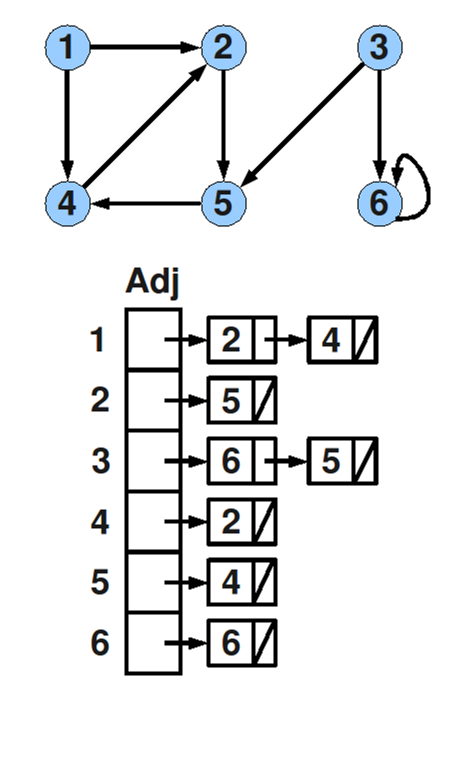
\includegraphics[width=10pc]{./imagens/adj-list-2.png}
\caption{Grafo na forma de lista de adjacência}
\label{fig_adj}
\textit{Fonte: Adaptado de \cite{nonato2000}}
\end{figure}

A representação de um grafo simples na forma CSR pode ser feita com apenas 2 vetores. Um deles contendo a concatenação em ordem de todas as listas de adjacências do grafo, e um segundo vetor contendo um índice com a posição de início da lista de adjacência de cada vértice. Uma representação visual dessa estrutura pode ser vista na Figura~\ref{fig_csr}.

\begin{figure}[h]
\centering
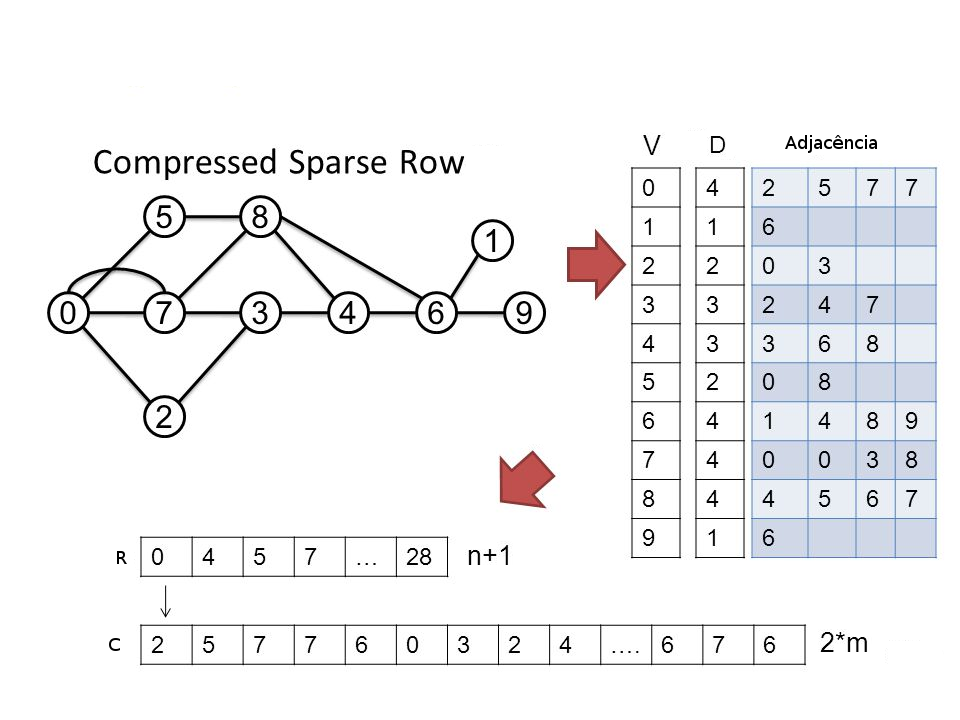
\includegraphics[width=20pc]{./imagens/csr-exemplo.png}
\caption{Grafo na forma compacta}
\label{fig_csr}
\textit{Fonte: Adaptado de \cite{kamesh2011}}     
\end{figure}


A escolha do particionamento do problema é um fator importante no incremento da performance do processamento paralelo. O ideal é uma estratégia que utilize sabiamente a quantidade de \textit{threads} existentes, de modo que o trabalho executado esteja balanceado \cite{Hong2011b,Hong2011a}. Inicialmente foram investigados três abordagens: uma \textit{thread} pra cada grafo, um bloco de \textit{threads} para cada grafo e uma \textit{thread} para cada vértice.

Analisamos essas três abordagens aplicando a grafos de até 20 vértices de um banco de grafos \cite{hog2013}. 
Após a avaliação, apesar de praticamente todas serem abordagens mais rápidas que uma implementação serial, 
até as melhores apresentaram algum tipo de gargalo em alguma etapa. Com isso, escolhemos uma combinação da abordagem de grafo/bloco com grafo/vértice  para trazer os benefícios de cada uma das abordagens, 
minimizando as possíveis ineficiências de cada. Com esse objetivo,
foi desenvolvido o Algoritmo \ref{alg-heurístico-abordagem-hibrida}, com dois núcleos. 

O primeiro núcleo, chamado de \textit{Kernel-1}, particiona o trabalho do grafo em blocos inteiros. Caso um bloco não seja totalmente utilizado, esse trabalho fracionado ficará a cargo do segundo núcleo, também chamado de \textit{Kernel-2}. Considere \textit{TAMBLOCK} a quantidade máxima de \textit{threads} ativas. Assim, o \textit{Kernel-1} trabalhará com grafos cuja a quantidade de vértices seja maior ou igual a um múltiplo do tamanho de \textit{TAMBLOCK}. O \textit{Kernel-2} agrupa o trabalho restante em blocos com tamanho múltiplo do \textit{TAMBLOCK}. 

O Algoritmo \ref{alg-heurístico-abordagem-hibrida} utiliza as abordagens grafo/bloco e vértice/\textit{thread} através dos núcleos 1 e 2 descritos anteriormente.

\begin{algorithm2e}
\SetAlFnt{\tiny}
\SetAlCapFnt{\small}
\SetAlCapNameFnt{\small}
\SetAlgoLined
\Entrada{$G_s$}
\Saida{Envoltória Aproximada de $G_s$}
\Inicio{
$ R_s \gets \emptyset $\\
$ M_w \gets \emptyset $\\
$ nblk \gets 0 $\\
$ TAMBLOCKTRUNC \gets TAMBLOCK $\\


\ParaCada{$g \in G_s$}{
  $n \gets |V(g)|$ \\
  $R_s[g] \gets n $\\
  \Se{$n \ge TAMBLOCK $}{
    $nblk \gets nblk + 1$\\
  }
  $nvtrunc \gets n$ {\bf mod} $TAMBLOCK $\\
  $tntrunc \gets tntrunc + vtrunk $\\        
  \Para{$i$ de $1$ até $nvtrunc$}{
	$v \gets \frac{n}{TAMBLOCK} \times TAMBLOCK + i$ \\
	$ M_w.add(\{g,v\})$\\
  }
}
$nblktrunc \gets \frac{nvertstrunk}{TAMBLOCKTRUNC}$\\
$kAproxEnvoltGrafBlk<<<nblk, TAMBLOCK>>>(G_s, R_s)$\\
$kAproxEnvGrafBlkTrunc<<<nblktrunc, TAMBLOCKTRUNC>>>(G_s, R_s, M_w, tntrunc)$\\
\Retorna{$R_s$}
}
\caption{HeurísticoNEnvoltorioPCombinado}
\label{alg-heurístico-abordagem-hibrida}
\end{algorithm2e}



\begin{algorithm2e}
\SetAlFnt{\tiny}
\SetAlCapFnt{\small}
\SetAlCapNameFnt{\small}
\SetAlgoLined
\Entrada{$G_s$}
\Saida{Nº Envoltório Aproximado $R_s$ }	
    $shared$ $rlocal$\\			
	\Se{$threadIdx = 0$}{
    	$rlocal \gets \infty$\\
    }
    $syncthreads()$\\
	$g \gets G_s[blockIdx]$\\
    $n \gets |V(g)|$\\
    $id \gets threadIdx$\\        
    $i \gets 0$\\
    \Enqto{
    	$id < n$
    }{
    	$v \gets id$\\
        $S^\prime \gets \{v\}$\\                                
        \Enqto{$|H(g,S^\prime)| < n$}{
            $ve \gets \emptyset$\\ 
            $mHs \gets ncve \gets 0$\\
            \ParaCada{$w \in V(g)-S^\prime$}{
                $S_{aux} \gets S^\prime \cup \{w\}$\\
                $tHs \gets |H(g,S_{aux})|$\\
                \Se{$tHs \ge mHs \land |Adj[w]| > ncve$}{
                    $v_e \gets w$\\
                    $mHs \gets tHs$\\
                    $ncve \gets  |Adj[w]| $\\
                }
            }{$S^\prime \gets S^\prime \cup \{v_e\}$}
        }
        
        $i \gets i + 1$\\
        $id \gets id + (i \times TAMBLOCK)$\\
    }
		$syncthreads()$\\
    \Se{$threadIdx = 0$}{
    	$R_s[g]=rlocal$\\
    }
\caption{kAproxEnvoltGrafBlk}
\label{alg:heurístico-numero-envoltoria-p3-mix}
\end{algorithm2e}

\begin{algorithm2e}
\SetAlFnt{\tiny}
\SetAlCapFnt{\small}
\SetAlCapNameFnt{\small}
\SetAlgoLined
\Entrada{$G_s$, $M_w$, $tntrunc$}
\Saida{Nº Envoltório Aproximado $R_s$ }
$id \gets blockIdx + threadIdx$\\
$i \gets 0$\\
\Enqto{
$id < tntrunc$
}{
$g \gets M_w[id][0]$\\
$v \gets M_w[id][1]$\\
%exapandHullSetFromV\\
$S^\prime \gets \{v\}$\\
\Enqto{$|H(g,S^\prime)| < n$}{
    $ve \gets \emptyset$\\
    $mHs \gets ncve \gets 0$\\
    \ParaCada{$w \in V(g)-S^\prime$}{
        $S_{aux} \gets S^\prime \cup \{w\}$\\
        $tHs \gets |H(g,S_{aux})|$\\
        \Se{$tHs \ge mHs \land |Adj[w]| > ncve$}{
            $v_e \gets w$\\
            $mHs \gets tHs$\\
            $ncve \gets  |Adj[w]| $\\
        }
    }{$S^\prime \gets S^\prime \cup \{v_e\}$}
}
$i \gets i + 1$\\
$id \gets id + (i \times TAMBLOCKTRUNC)$\\
$atomicMin(R_s[g],|S^\prime|)$\\
}
\caption{kAproxEnvGrafBlkTrunc}
\end{algorithm2e}



\begin{figure}[h]
\centering
\begin{tikzpicture}
  \begin{axis}
  [xlabel={Quantidade de grafos}, ylabel={Tempo(s)},legend pos=north west,axis lines=left]
  \addplot[name path=maxi,mark=none,blue] coordinates {
  (6,0) (48,10.1) (96,10.2) (384,40.1) (620,57.5) (1024,70.3) 
  };
  \addlegendentry{serial}
  
  \addplot[name path=maxi,mark=none,red] coordinates {
  (6,0) (48,303) %(96,608) %(384,0) (620,0) (1024,0) 
  };
  \addlegendentry{grafo/thread}

  \addplot[name path=maxi,mark=none,green] coordinates {
  (6,0) (48,12.5) (96,12.6) (384,15.3) (620,38.6) (1024,38.7) 
  };
  \addlegendentry{grafo/bloco}

  \addplot[name path=maxi,mark=none,yellow] coordinates {
  (6,0) (48,3.6) (96,4.3) (384,13.8) (620,37.1) (1024,37.4) 
  };
  \addlegendentry{vertice/thread}
  
  \addplot[name path=maxi,mark=none] coordinates {
  (6,0) (48,3.6) (96,13) (384,17.3) (620,37.1) (1024,38.8) 
  };
  \addlegendentry{combinada}
  \end{axis}
\end{tikzpicture}
\caption{Crescimento heurístico}
\label{fig-crescimento-num-heurístico}
\end{figure}

Com essa abordagem combinada, conseguimos melhorar os tempos de execução em pelo menos quatro vezes,
conforme podemos ver no gráfico da Figura~\ref{fig-crescimento-num-heurístico} e na Tabela~\ref{tab-speedups-paralelos}.

\begin{table}[H]
\centering
\caption{Tempo de execução das implementações aproximativas paralelas}
\label{tab-speedups-paralelos}
\begin{tabular}{l|l|l|l|l|}
\cline{2-5}
                                              & \multicolumn{4}{l|}{\textbf{Tempo em segundos de execução}}                            \\ \hline
\multicolumn{1}{|l|}{\textbf{Estrategia}}     & \textbf{100 grafos} & \textbf{300 grafos} & \textbf{600 grafos} & \textbf{1000 grafos} \\ \hline
\multicolumn{1}{|l|}{\textbf{grafo/thread}}   & 303                 & -                   & -                   & -                    \\ \hline
\multicolumn{1}{|l|}{\textbf{grafo/bloco}}    & 12.6                & 15.3                & 38.6                & 38.7                 \\ \hline
\multicolumn{1}{|l|}{\textbf{vértice/thread}} & 4.3                 & 13.8                & 37.1                & 38.4                 \\ \hline
\multicolumn{1}{|l|}{\textbf{combinada}}      & 13                  & 17.3                & 37.1                & 37.4                 \\ \hline
\end{tabular}
\end{table}


\section{Ferramenta Desenvolvida: FATIG}

Ao decorrer da execução do trabalho, uma ferramenta foi desenvolvida para facilitar a utilização dos algoritmos implementados, visualização e consulta histórica dos resultados obtidos. Apresentaremos a FATIG - {\it F}erramenta {\it A}berta para {\it T}estes e {\it I}mplementações para {\it P}roblemas em {\it G}rafos.
Apesar de não ser o objetivo do trabalho, deixaremos aqui uma visão geral de como usar e as tecnologias empregadas. 
E a quem puder interessar, estará disponível um código e um \textit{livedemo}.

%\subsection{Modo de Usar}
A FATIG pode ser acessada por qualquer navegador web. O usuário pode fornecer um arquivo com um grafo de interesse,
ou gerar um dentre os geradores disponíveis. 
Com algum grafo carregado o usuário pode executar 
qualquer problema das categorias fornecidas e
visualizar o resultado ao termino da execução. No Apêndice~\ref{apend-ferramenta},
temos figuras da tela principal da FATIG com mais detalhes.


% \begin{figure}[h]
% \begin{center}
% 	\caption{Ferramenta para Execução de Algoritmos}
%     \label{fig-ferramenta-grafo}
% 	\begin{center}
% 	    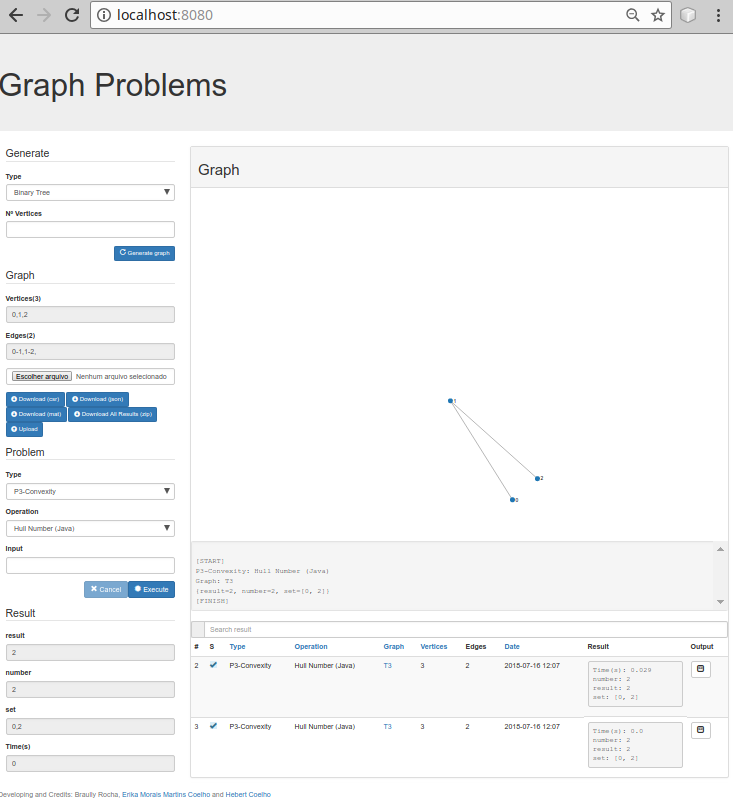
\includegraphics[width=0.8\textwidth]{./imagens/ferramenta-tela-principal.png}
% 	\end{center}
% \end{center}
% \end{figure}


Neste trabalho foram implementados geradores de grafos para árvore binárias, estritamente binárias, blocos, ciclos, completos,
completos bipartido, caminhos e rodas. Basta selecionar o tipo, informar os parâmetros e mandar gerar no botão \textit{Genearte graph}.

O grafo gerado pode ser baixado nos formatos matriz de adjacência ou linha de adjacência compacta, nos botões \textit{Download (mat)} e \textit{Download (csr)} respectivamente.

Para conveniência e mais testes de interesse do trabalho, 
também foram implementados: um gerador de grafos aleatórios; um gerador a partir de uma lista de arestas; gerador a partir de um código $G6$ \cite{Brendan2015}; e por um último um gerador a partir de um índice lexicográfico de combinações de arestas.

%Geradores de Grafos e Entradas de Grafos em Diversos Formatos
Os resultados de todas as execuções, estão disponíveis na tabela de resultados que fica na parte inferior da tela da aplicação. 
Na tabela temos a informação da data de execução,
a operação realizada, um link para \textit{download} do grafo usado,
a quantidade de vértices e arestas, e a resposta da operação realizada.

Os algoritmos propostos neste trabalho, foram implementados e estão disponíveis para uso na ferramenta. A Tabela~\ref{tabela-implementacao} relaciona a operação com o respectivo algoritmo apresentado neste capítulo. Alguns algoritmos auxiliares também foram implementados e estão listados na tabela.

\begin{table}[H]
\caption{Implementações Disponíveis na F.A.T.I.G.}
\label{tabela-implementacao}
\begin{tabular}{|l|l|l|l|}
\hline
\multicolumn{4}{|c|}{\textbf{Operação Implementada}}       \\ \hline
\textbf{Seção}  & \textbf{Nome}  & \textbf{Linguagem}  & \textbf{Algoritmo} \\ \hline
\multirow{11}{*}{ \rotatebox[origin=c]{90}{\textit{P3-Convexity}}} & H(S)                      & Java                                & \ref{alg:fecho-p3}                                                             \\ \cline{2-4} 
                               & Hull Number (Java)        & Java                                & \ref{alg:numero-envoltoria-p3}                                                 \\ \cline{2-4} 
                               & Hull Number Serial        & C                                   & \ref{alg:numero-envoltoria-p3}                                                 \\ \cline{2-4} 
                               & Hull Number Parallel      & CUDA                                & \ref{alg:numero-envoltoria-p3}                                                 \\ \cline{2-4} 
                               & Hull Number Heuristic     & Java                                & \ref{alg:heurístico-numero-envoltoria-p3}                                    \\ \cline{2-4} 
                               & Hull Number Heuristic Mix & CUDA                                & \ref{alg:heurístico-numero-envoltoria-p3-mix}                                \\ \cline{2-4} 
                               & Check Caratheodory Set(S) & Java                                & \ref{alg:conjunto-caratheodory-p3}                                             \\ \cline{2-4} 
                               & Nº Caratheodory (Binary)  & Java                                & \ref{alg:numero-caratheodory-p3}                                               \\ \cline{2-4} 
                               & Nº Caratheodory Serial    & C                                   & \ref{alg:numero-caratheodory-p3}                                                \\ \cline{2-4} 
                               & Nº Caratheodory Parallel  & CUDA                                & \ref{alg:numero-caratheodory-p3}                                                 \\ \cline{2-4} 
                               & Nº Caratheodory Heuristic & CUDA                                & \ref{alg:heurístico-numero-caratheodory-p3}                                     \\ \hline
\multirow{3}{*}{ \rotatebox[origin=c]{90}{\textit{General}}}       & BFS                       & Java                                & Busca em Largura                                                                                \\ \cline{2-4} 
                               & Statistic                 & Java                                & Cintura, diâmetro e maior grau                                                           \\ \cline{2-4} 
                               & Subgraph                  & Java                                & Subgrafo induzido                                              \\ \hline
\end{tabular}
\end{table}

\subsection{Ferramentas e Bibliotecas utilizadas}
No desenvolvimento da FATIG, foram utilizadas bibliotecas de terceiros para reduzir o tempo necessário da implementação 
e utilizar de boas práticas presentes em implementações já consolidadas.
Como toda aplicação moderna, podemos separa a implementação em duas partes
o \textit{Front-end} e \textit{Back-end}.

Como o objetivo da FATIG era facilitar a execução e visualização de problemas em grafos,
o \textit{Front-end} foi desenvolvido em \textit{HTML5}. Justamente para que possa ser acessível a praticamente qualquer estação de trabalho com um navegador \textit{Web}.
Os componentes básicos como botões, caixas de seleção, tabelas e outros foram 
aprimorados com a biblioteca \textit{Bootstrap} \cite{bootstrap}, para um melhor visual
e uma interface responsiva. Para visualização e manipulação dos grafos,
a biblioteca D3JS \cite{d3js} foi empregada, pois possui diversas facilidades para visualização de documentos e dados.
Neste trabalho usamos especificamente recursos para \textit{force graph undirected} \cite{d3jsforce}. Por fim usamos o \textit{Angular JS} \cite{angularjs} para intermediar a comunicação do \textit{Front-end} com o \textit{Back-end}.

No \textit{Back-end} utilizamos a Linguagem \textit{Java} em sua versão 8 e a biblioteca \textit{Java Universal Network/Graph} \cite{jung},
que além de fornecer estruturas de dados para manipulação de grafos contem diversos algoritmos já implementados tais como busca em largura, \textit{Dijkstra}, arvore de busca e diversos outros. 
Por fim usamos a biblioteca Jersey \cite{jersey} para fornecer uma interface de \textit{web service} e para estabelecer a ponte de comunicação com o \textit{Front-end}.

\subsection{Customização e Extensão}
As operações implementadas neste trabalho
estão todas disponíveis na pasta \textit{operation} do codigo fonte
e podem ser livremente estudadas e modificadas a quem interessar.

A criação de uma nova operação é simples. A classe deve ser colocada na mesma pasta \textit{operation}, e deve implementar a interface \textit{IGraphOperation}. 
O contrato da interface exige a implementação de três métodos, dois deles devem simplesmente retornar, respectivamente, o nome da operação e a categoria. E o terceiro recebe um grafo e deve retornar, o resultado desejado da operação em um mapa de \textit{String}.

Após a criação ou alteração de uma operação, a aplicação precisa ser compilada novamente e reiniciada.
Com isso a nova operação já estará disponível para uso no \textit{Front-end},
sem necessidade de maiores ajustes.

Assim como as operações, os geradores utilizados neste trabalho estão disponíveis e podem ser acessados na pasta \textit{generator} do código fonte. Tal qual as operações, os geradores podem ser criados e alterados, basta implementar a interface \textit{IGraphGenerator}. O novo gerador deverá implementar métodos que forneça uma descrição do gerador, a lista de parâmetros necessários e o método que ira gerar o grafo a partir dos parâmetros solicitados.

Uma das facilidades do \textit{Back-end} é despachar a execução
de uma operação para um outro programa em aplicação,
como é o caso de uma implementação em outra linguagem. 
As implementações em \textit{CUDA} deste trabalho,
devem ser compiladas e executadas em um hospedeiro 
com uma placa de vídeo \textit{NVidia}. 
Uma vantagem de nossa ferramenta, é poder usar implementações executando remotamente em outras estações.

As implementações desenvolvidas em \textit{CUDA} e Linguagem \textit{C/C++}, 
estão disponíveis na pasta \textit{c-projects}. 
Cada implementação deve estar em uma pasta própria,
contendo um arquivo \textit{Makefile} com as instruções para sua compilação
e um outro arquivo chamado \textit{Descritor} que contém as informações
do nome e tipo do problema, para ser disponibilizado no \textit{Front-end}.
Nessa pasta além das implementações existem dois projetos em branco,
um \textit{C} e outro em \textit{C++}. Assim como para uma operação em \textit{Java}, 
basta que a ferramenta seja recompilada e iniciada, 
para que as novas implementações estejam acessíveis.

\subsection{Resultados teóricos obtidos com a FATIG}
Os resultados teóricos deste trabalho foram investigados a partir de resultados práticos explorados de um banco de grafos processados pela FATIG.
A coletânea de grafos utilizada está disponível em House of Graphs \cite{hog2013} no meta-diretório de grafos. 
Grande parte da coletânea utilizada é composta por todos os possíveis grafos de uma certa classe
específica até um número x de vértices. 
Todos livres de isomorfismo. 

A Tabela~\ref{tab-banco-testes} mostra a quantidade de grafos investigados com a FATIG, separados por classes e quantidades de vértices. Na coluna {\bf Quantidade Carathéodory} exibimos a quantidade de grafos que foram calculado o número de Carathéodory e na coluna {\bf Quantidade Envoltório} exibimos a quantidade de grafos que foram calculados o número envoltório.

\begin{table}[H]
\centering
\caption{Quantitativo de Grafos Executados e Analisados}
\label{tab-banco-testes}
\begin{tabular}{r|r|r|r|l}
\textbf{Classe Grafos} & \textbf{\begin{tabular}[c]{@{}l@{}}Extensão\\ de Vértices\end{tabular}} 
                       & \textbf{\begin{tabular}[c]{@{}l@{}}Quantidade\\Carathéodory \end{tabular}}    
                       & \textbf{\begin{tabular}[c]{@{}l@{}}Quantidade\\Envoltório\end{tabular}}    
                       & \textbf{Referência} \\ \hline
Hipo-hamiltoniano         & 10-24    & 3.379  & 3.379        & \cite{Aldred1997,hog2013,Goedgebeur2016a} \\
Quase hipo-hamiltoniano  & 17-32    & 688 & 831          & \cite{hog2013,Goedgebeur2016} \\
Crítico sem H         & 4-16     & 1.041 & 1.041        & \cite{Chudnovsky2015,hog2013,Goedgebeur2015} \\
Maximal sem triangulo  & 3-30     & 1.536.047     & 1.536.047 & \cite{Brandt1998,Brandt2000,hog2013,Liu2015} \\
Fortemente regular        & 25-40    & 43.669 & 43.669       & \cite{hog2013,spence12} \\
Cúbico                   & 4-32     & 241.705 & 3.964.513      & \cite{Brinkmann2011,Brinkmann1995,hog2013,Robinson1983} \\
Quártico                 & 5-37     & 122.583 & 138.427      & \cite{hog2013,Meringer2009} \\
Snarks                  & 10-32    & 3.493 & 9.623         & \cite{Brinkmann2013,hog2013} \\
Vértice-transitivo      & 3-31    & 19.260 & 37.477        & \cite{hog2013,Royle1997} \\
Minimal Ramsey(3,k)          & 16-35    & 6.972 & 76.697        & \cite{hog2013,Goedgebeur2012,Rochester2017}             \\
Nº de Ramsey R(K3,G)         & 10-36      & 1.628.788  & 1.628.788     &  \cite{Brinkmann2012,hog2013,Rochester2017} \\
Árvores                   & 3-20     & 874.321  & 874.321     & \cite{hog2013,Li99} \\ \hline
\multicolumn{2}{r|}{Total} & 4.481.946         & \multicolumn{2}{l}{8.314.813} \\
\multicolumn{2}{r|}{Tempo força bruta:} & 240h         & \multicolumn{2}{l}{41h} \\
\multicolumn{2}{r|}{Tempo heurístico:} & 17h         & \multicolumn{2}{l}{2h} \\
\end{tabular}
\end{table}

%Apesar de terem apresentados para grafos densos ganhos de performance de 3 a 4 \textit{speedups} em relação a solução sequencial. Os resultados comparativos da implementação paralela não foram contabilizados nessa análise.
%Por não conter as melhorias da versão sequencial e o formato utilizado no histórico de resultados não estava adequado para comparação com os demais algoritmos. Os resultados são referentes aos grafos descritos no banco de grafos coletado.

Os resultados aproximados, vindos da abordagem heurística tiveram bons resultados, na Tabela~\ref{tab:resultado-aproximado-heuristicas} temos um resumo deles. Em sua grande maioria os resultado de mais de 90\% dos grafos foi exatamente o resultado real. 



\begin{table}
    \caption{Desempenho dos resultados aproximados}
    \label{tab:resultado-aproximado-heuristicas}
    \centering
   \begin{tabular}{r|r|r|r}
    \textbf{Classe Grafos}    & \textbf{\begin{tabular}[c]{@{}l@{}}Extensão\\ de Vértices\end{tabular}}
          & \textbf{\begin{tabular}[c]{@{}l@{}}Aproximativo\\Carathéodory\end{tabular}}
          & \textbf{\begin{tabular}[c]{@{}l@{}}Aproximativo\\Envoltório\end{tabular}} \\ \hline
Crítico sem H         & 4-16  & \begin{tabular}[r]{@{}r@{}}1.041\\(>90\%)\end{tabular} & \begin{tabular}[r]{@{}r@{}}1.041\\(>90\%)\end{tabular}      \\ \hline
Maximal sem triangulo & 3-30  & \begin{tabular}[r]{@{}r@{}}1.536.047\\(>90\%)\end{tabular} & \begin{tabular}[r]{@{}r@{}}1.536.047\\(>90\%)\end{tabular} \\ \hline
Fortemente regular    & 25-40 & \begin{tabular}[r]{@{}r@{}}43.669\\ (100\%)\end{tabular}         &  \begin{tabular}[r]{@{}r@{}}43.669\\ (100\%)\end{tabular} \\ \hline
Quártico              & 5-37  & \begin{tabular}[r]{@{}r@{}}122.583\\ (>70\%)\end{tabular}  & \begin{tabular}[r]{@{}r@{}}138.427\\ (>70\%)\end{tabular} \\ \hline
Snarks                & 10-32 & \begin{tabular}[r]{@{}r@{}}3.493\\ (>80\%)\end{tabular}  & \begin{tabular}[r]{@{}r@{}}9.623\\ (>80\%)\end{tabular}      \\ \hline
Vértice-transitivo    & 3-31  & 19.260 (--)      & 37.477  (>95\%)      \\
    \end{tabular}
\end{table}


Desta averiguação exploratória, identificamos conjecturas para os grafos fortemente regulares e maximais sem triângulo. Estas duas classes foram investigadas mais profundamente no decorrer do trabalho, frutificando em resultados teóricos apresentados nos capítulos 3 e 4. Os resultados referentes ao número envoltório foram inclusive estendidos para grafos de diâmetro 2.


Os resultados práticos dessas duas classes, estão apresentadas aqui como um gráfico e uma tabela com o resumo dos resultados da execução do algoritmo força bruta em comparação com o versão heurístico. Nas tabelas temos as seguintes colunas:
\begin{itemize}
   \item{\textbf{Nº de vértices}: que contém a quantidade de vértices dos grafos testados;}
   \item{\textbf{Quantidade}: que contém de grafos testados em relação a quantidade de vértices. Se necessário poderá
         conter um valor percentual entre parentes que indica  quantidade executada em relação ao total existente,
         daquele tipo de grafo;}
    \item{\textbf{c(G)} ou \textbf{h(G)} indica o intervalo ao qual o resultado do parâmetro cai;}
    \item{\textbf{T$_1$(s)}: é o tempo de execução total do algoritmo força bruta
           para todos os grafos executados;}
    \item{\textbf{Acertos}: refere-se a porcentagem de resultados aproximados coincidentes com o resultado exato;}
    \item{\textbf{max$\{\Delta (r)\}$} é maior diferença encontrada, entre um resultado aproximado e o resultado real;}
    \item{\textbf{T$_2$(s)}: é o tempo total de execução total da versão aproximativa para todos os grafos executados.}
\end{itemize}

Dado essa visão de como os resultados práticos serão apresentados, podemos ver na Tabela~\ref{tab-comparativo-strongly-regular} que o número de Carathéodory para o banco de grafos não ultrapassou o valor 2 e o algoritmo heurístico teve um bom índice de acertos.

\begin{table}[h]
\centering
\caption{Resultados $c(G)$ grafos fortemente regular}
\label{tab-comparativo-strongly-regular}
\begin{tabular}{r|r|r|r|r|r|r}
\textbf{} & \multicolumn{3}{c|}{\textbf{\begin{tabular}[c]{@{}c@{}}Algoritmo \ref{alg:numero-caratheodory-p3} \\ $NumeroCaratheodory$\end{tabular}}} 
& \multicolumn{3}{c}{\textbf{\begin{tabular}[c]{@{}c@{}}Algoritmo \ref{alg:heurístico-numero-caratheodory-p3} \\ $AproxNCaratheodory$\end{tabular}}} \\ \hline
\textbf{Nº Vert.} & \textbf{Quantidade} & \textbf{c(G)} & \textbf{$T_1(s)$} & \textbf{Acertos} & \textbf{max$\{\Delta(r)\}$} & \textbf{$T_2(s)$} \\ \hline
25 & 16 (amostras)    & 2 & 0,75      & 100,0\% & 0  & 0,43    \\
26 & 10 (amostras)    & 2 & 0,4       & 100,0\% & 0  & 0,24    \\
27 & 1 (amostras)     & 2 & 0,05      & 100,0\% & 0  & 0,03    \\
28 & 4 (amostras)     & 2 & 46,79     & 50,0\%  & 0  & 0,12    \\
29 & 41 (amostras)    & 2 & 2,55      & 100,0\% & 0  & 1,71    \\
35 & 4081 (amostras)  & 2 & 586,06    & 100,0\% & 0  & 271,46  \\
36-40 & 39516 (amostras) & 2 & 221769,58   & --  & --  & -- \\
\end{tabular}
\end{table}


Para o número envoltório a Tabela~\ref{tab-comparativo-hn-sr} mostra que $h(G)=2$ para os grafos fortemente regulares testados e o algoritmo heurístico teve um acerto de 100\%.


\begin{table}[h]
\caption{Resultados h(G) grafos fortemente regular}
\label{tab-comparativo-hn-sr}
\begin{tabular}{r|r|r|r|r|r|r}
\textbf{} & \multicolumn{3}{c|}{\textbf{\begin{tabular}[c]{@{}c@{}}Algoritmo \ref{alg:numero-envoltoria-p3} \\ $NumeroEnvoltorio$\end{tabular}}} 
          & \multicolumn{3}{c}{\textbf{\begin{tabular}[c]{@{}c@{}}Algoritmo \ref{alg:heurístico-numero-envoltoria-p3} \\ $AproxNEnvoltoria$\end{tabular}}} \\ \hline
\textbf{Nº Vert.} & \textbf{Quantidade} & \textbf{h(G)} & \textbf{$T_1(s)$} & \textbf{Acertos} & \textbf{max$\{\Delta(r)\}$} & \textbf{$T_2(s)$} \\ \hline
25 & 16 (amostras)    & 2 & 0,01 & 100,0\% & 0 & 0,07   \\
26 & 10 (amostras)    & 2 & 0    & 100,0\% & 0 & 0,02   \\
27 & 1 (amostras)     & 2 & 0    & 100,0\% & 0 & 0,01   \\
28 & 4 (amostras)     & 2 & 0    & 100,0\% & 0 & 0,01   \\
29 & 41 (amostras)    & 2 & 0,01 & 100,0\% & 0 & 0,16   \\
35 & 4081 (amostras)  & 2 & 0,15 & 100,0\% & 0 & 30,96  \\
36-40 & 39516 (amostras) & 2 & 0,82 & 100,0\% & 0 & 280,13 \\
\end{tabular}
\end{table}

Na Tabela~\ref{tab-comparativo-mtf} vemos os resultados da execução do algoritmo de número de Carathéodory para os grafos maximais sem triângulo. Podemos observar que $c(G)$ não ultrapassou a constante 4 e o algoritmo heurístico teve um índice de acertos acima de 90\%.

\begin{table}[h]
\caption{Resumo dos resultados $c(G)$ para grafos MST}
\label{tab-comparativo-mtf}
\begin{tabular}{r|r|r|r|r|r|r}
\textbf{} & \multicolumn{3}{c|}{\textbf{\begin{tabular}[c]{@{}c@{}}Algoritmo \ref{alg:numero-caratheodory-p3} \\ $NumeroCaratheodory$\end{tabular}}} 
          & \multicolumn{3}{c}{\textbf{\begin{tabular}[c]{@{}c@{}}Algoritmo \ref{alg:heurístico-numero-caratheodory-p3} \\ $AproxNCaratheodory$\end{tabular}}} \\ \hline
\textbf{Nº Vert.} & \textbf{Quantidade} & \textbf{c(G)} & \textbf{$T_1(s)$} & \textbf{Acertos} & \textbf{max$\{\Delta(r)\}$} & \textbf{$T_2(s)$} \\ \hline
    3-5  & 6 (100\%)       & 2         & 0        & 100,0\% & 0 & 0      \\
    6-9  & 36 (100\%)      & {[}2,3{]} & 0,01  & 80,5\% & 1 & 0,01      \\
  10-18  & 1.535.202 (100\%) & {[}2,4{]} & 29.529    & 98,13\% & 1 & 6.863   \\
  19-30 & 803 (amostras) & {[}2,3{]} & 6.496    & 95,76\%  & 1 & 11,64 
\end{tabular}%
\end{table}

\begin{figure}[h]
\centering
\begin{tikzpicture}
\begin{axis}
    [xlabel={Nº de Vértices}, ylabel={Nº de Carathéodory}, 
     legend pos=north west,clip=false,axis lines=left,
     ymin=1, ymax=5, ytick={2,3,4,5},
     xtick={2,6,10,18,30}]
     \addplot[name path=maxi,color=red,mark=none] coordinates {
        (3,1.98) (18,1.98) 
     };
     \addplot[name path=mini,color=blue,mark=none] coordinates {
        (3,2) (5,2) (6,3) (10,4) (18,4)
     };
     \addlegendentry{mínimo}
     \addlegendentry{máximo}
     \addplot[dotted, name path=miniaprox,color=red] coordinates {
        (18,2) (30,2)
     };
    \addplot[dotted, name path=maxaprox,color=blue] coordinates {
        (18,4) (19,3) (30,3) 
     };
     \addplot[fill=blue, fill opacity=0.3] fill between[of=maxi and mini];
\end{axis}
\end{tikzpicture}%
\caption{Nº de Carathéodory para grafos MST}
\label{fig-ncarat-mst}
\end{figure}

\begin{table}[h]
\caption{Resumo dos resultados $h(G)$ para grafos MST}
\label{tab-comportamento-hn-mtf}
    \begin{tabular}{r|r|r|r|r|r|r}
    \textbf{} & \multicolumn{3}{c|}{\textbf{\begin{tabular}[c]{@{}c@{}}Algoritmo \ref{alg:numero-envoltoria-p3} \\ $NumeroEnvoltorio$\end{tabular}}} 
              & \multicolumn{3}{c}{\textbf{\begin{tabular}[c]{@{}c@{}}Algoritmo \ref{alg:heurístico-numero-envoltoria-p3} \\ $AproxNEnvoltoria$\end{tabular}}} \\ \hline
    \textbf{Nº Vert.} & \textbf{Quantidade} & \textbf{h(G)} & \textbf{$T_1(s)$} & \textbf{Acertos} & \textbf{max$\{\Delta(r)\}$} & \textbf{$T_2(s)$} \\ \hline
	3  & 1 (100\%)       & 2  & 0     & 100,0\% & 0 & 0    \\
	4  & 2 (100\%)       & {[}2,3{]}  & 0     & 100,0\% & 0 & 0    \\
	5  & 3 (100\%)       & {[}2,4{]}  & 0     & 100,0\% & 0 & 0    \\
	6  & 4 (100\%)       & {[}2,5{]}  & 0     & 100,0\% & 0 & 0    \\
	7  & 6 (100\%)       & {[}2,6{]}  & 0     & 100,0\% & 0 & 0    \\
	8  & 10 (100\%)      & {[}2,7{]}  & 0     & 100,0\% & 0 & 0    \\
	9  & 16 (100\%)      & {[}2,8{]}  & 0     & 93,8\%  & 1 & 0     \\
	10 & 31 (100\%)      & {[}2,9{]}  & 0,01  & 90,3\%  & 1 & 0,01  \\
	11 & 61 (100\%)      & {[}2,10{]} & 0     & 91,8\%  & 1 & 0,01 \\
	12 & 147 (100\%)     & {[}2,11{]} & 0,01  & 94,6\%  & 1 & 0,02 \\
	13 & 392 (100\%)     & {[}2,12{]} & 0     & 97,2\%  & 1 & 0,08 \\
	14 & 1.274 (100\%)    & {[}2,13{]} & 0,01  & 98,4\%  & 1 & 0,26 \\
	15 & 5.036 (100\%)    & {[}2,14{]} & 0,05  & 98,8\%  & 1 & 1,33  \\
	16 & 25.617 (100\%)   & {[}2,15{]} & 0,19  & 99,0\%  & 1 & 8,47  \\
	17 & 164.796 (100\%)  & {[}2,16{]} & 1,16  & 99,4\%  & 1 & 66,76 \\
	18 & 1.337.848 (100\%) & {[}2,17{]} & 10,51 & 99,7\%  & 1 & 655,39 \\
     19-30 & 803 (amostras)             & {[}2,3{]}          & 1,31 & 99,2\%   & 1 & 0,21
    \end{tabular}%   
\end{table}

\begin{figure}[h]
\centering
\begin{tikzpicture}
    \begin{axis}
        [xlabel={Nº de Vértices}, ylabel={Nº Envoltório}, 
         legend pos=north west,clip=false,axis lines=left,
         ymin=1, ymax=19, ytick={2,3,4,5,6,7,8,9,10,11,12,13,14,15,16,17},
         xtick={3,5,7,9,11,13,15,18,30}]
         \addplot[name path=maxi,color=red,mark=none] coordinates {
            (3,1.98) (18,1.98)
         };
         \addplot[name path=mini,color=blue,mark=none] coordinates {
            (3,2) (4,3) (5,4)
            (6,5) (7,6) (8,7)
            (9,8) (10,9) (11,10) 
            (12,11) (13,12) (14,13)
            (14,13) (15,14) (16,15)
            (17,16) (18,17)
         };
         \addplot[fill=blue, fill opacity=0.3] fill between[of=maxi and mini];
         \addlegendentry{mínimo}
         \addlegendentry{máximo}
         \addplot[dotted, name path=miniaprox,color=red] coordinates {
            (18,1.98) (30,1.98)
         };
        \addplot[dotted, name path=maxaprox,color=blue] coordinates {
            (18,17) (19,3) (30,3) 
         };
    \end{axis}
\end{tikzpicture}
\caption{Resultados h(G) para MST}
\label{fig-comportamento-hn-mtf}
\end{figure}

Para o número envoltório a Tabela~\ref{tab-comportamento-hn-mtf} mostra que este valor está sempre limitado a $n-1$, onde $n$ é o número de vértices.  Porém, analisando detalhadamente os resultados, é identificável que pra cada tamanho de vértice
existe apenas um grafo que atinge esse limite, o grafo estrela. 

Retirando o grafo estrela dos testes, identificamos que o número envoltório ficou limitado a 3 conforme ilustra a Tabela~\ref{tab-comparativo-hn-mtf-sem-estrela}.

\begin{table}[h]
    \caption{Resultados h(G) grafos MST$-\star$}
    \label{tab-comparativo-hn-mtf-sem-estrela}
    \begin{tabular}{r|r|r|r|r|r|r}
    \textbf{} & \multicolumn{3}{c|}{\textbf{\begin{tabular}[c]{@{}c@{}}Algoritmo \ref{alg:numero-envoltoria-p3} \\ $NumeroEnvoltorio$\end{tabular}}} 
              & \multicolumn{3}{c}{\textbf{\begin{tabular}[c]{@{}c@{}}Algoritmo \ref{alg:heurístico-numero-envoltoria-p3} \\ $AproxNEnvoltoria$\end{tabular}}} \\ \hline
    \textbf{Nº Vert.} & \textbf{Quantidade} & \textbf{h(G)} & \textbf{$T_1(s)$} & \textbf{Acertos} & \textbf{max$\{\Delta(r)\}$} & \textbf{$T_2(s)$} \\ \hline
	3  & 1 (100\%)       & 2  & 0     & 100,0\% & 0 & 0    \\
	4-18 & 1535228 (100\%)       & {[}2,3{]}  & 11,94     & 99,6\% & 1 & 732,23    \\
        19-30 & 803 (amostras)             & {[}2,3{]}          & 1,31 & 99,2\%   & 1 & 0,21
    \end{tabular}%
\end{table}

\begin{figure}[h]
\centering
\begin{tikzpicture}
    \begin{axis}
        [xlabel={Nº de Vértices}, ylabel={Nº Envoltório}, 
         legend pos=north west,clip=false,axis lines=left,
         ymin=1, ymax=4, ytick={0,1,2,3,4},
         xtick={3,5,7,9,11,13,15,18,30}]]
         \addplot[name path=maxi,color=red,mark=none] coordinates {
            (3,1.98) (18,1.98)
         };
         \addplot[name path=mini,color=blue,mark=none] coordinates {
            (3,2) (4,3) (18,3) 
         };
         \addplot[fill=blue, fill opacity=0.3] fill between[of=maxi and mini];
         \addlegendentry{mínimo}
         \addlegendentry{máximo}
         \addplot[dotted, name path=miniaprox,color=red] coordinates {
            (18,1.98) (30,1.98)
         };
        \addplot[dotted, name path=maxaprox,color=blue] coordinates {
            (18,3) (19,3) (30,3) 
         };
    \end{axis}
\end{tikzpicture}
\caption{Resultados $h(G)$ grafos MST$-\star$}
\label{fig-comparativo-hn-mtf-sem-estrela}
\end{figure}

Com base nesses resultados práticos, formulamos as conjecturas para número de Carathéodory e número envoltório em grafos fortemente regulares e maximais sem triângulo. Que mesmo não totalmente confirmadas e precisas, foram essenciais para ponto de partida das investigações teóricas mais aprofundadas deste trabalho. Outras conjecturas para outras classes de grafos foram levantadas, porém dado o tempo e escopo não foram exploradas, mas estão citadas como trabalhos futuros.

\subsection{Acesso ao Código}

O código da ferramenta pode ser obtido na página e/ou \textit{GitHub} dos autores \cite{braully2017}. %\url{https://github.com/braully/graph-problems-tool}
Pode ser compilado, baixado e executado. 
Instruções e requisitos para tal podem ser obtidos no próprio projeto. As operações implementadas estão executando para demonstração nos seguintes endereços:
\begin{itemize}
\item \url{http://gpt.braully.eti.br};
\item \url{http://www.inf.ufg.br/~hebert/grafos/};
\item \url{https://graph-problems-tool.herokuapp.com/};
\end{itemize}

Por motivos de recursos disponíveis, apenas as implementações em \textit{Java} e \textit{C} estão acessíveis na demonstração, para pequenos testes.


\chapter{Conclusões e Trabalhos Futuros}
\label{sec:crono}

Concluímos este trabalho com resultados teóricos e implementações de cunho mais prático, conforme visto nos capítulos anteriores. 

Primeiramente conseguimos delimitar um limite superior para o número envoltório de grafos de diâmetro 2. Caso o grafo de diâmetro 2 tenha um vértice de corte, demonstramos que o número envoltório é no máximo o número de componentes conexas do subgrafo removendo esse vértice. Para os demais grafos de diâmetro 2 desenvolvemos um algoritmo que iterativamente constrói um conjunto envoltório. Uma análise desse algoritmo, conjuntamente com propriedades desses grafos, nos permitiu limitar o tamanho máximo do conjunto envoltório concebido ao final. Com o estabelecimento deste limite geral para os grafos de diâmetro 2, conseguimos melhorá-lo para as subclasses fortemente regular, baseado nos parâmetros $b$ e $c$ e mostrando que o número envoltório dos maximal sem triângulo é no máximo 4. O que corroborou com as melhorias das premissas levantadas nos resultados da FATIG, culminando em resultados teóricos.

Nos experimentos realizados com a FATIG todos os grafos de diâmetro 2 testados tinham o número envoltório limitado a 4. Percebemos esse limite mas não conseguimos estabelecê-lo para a classe. Assim deixamos como trabalho futuro demonstrar a seguinte conjectura: 

\begin{conjecture}
    Seja $G$ um grafo com diâmetro 2, sem vértice de corte então $h(G) \le 4$.
    \label{conjecture-d2-4}
\end{conjecture}
 
Em nossas buscas o único grafo de diâmetro 2 sem vértice de corte, que atinge esse limite é o grafo de Hoffman Singleton. 
Na tentativa de encontrar um contraexemplo de um grafo de diâmetro 2, sem vértice de corte e com número envoltório maior ou igual a 5, nos deparamos múltiplas vezes com subcasos infindáveis. Porém como um efeito colateral dessa busca, desenvolvemos um algoritmo para geração dos grafos de Moore. Esse algoritmo utiliza fundamentos teóricos dos grafos de diâmetro 2 minimais e combinações de arestas. Apesar dos diversos trabalhos acadêmicos em busca pelo último grafo de Moore, pouco ou nada se documenta sobre o método pretendido. Dado o número de combinações e o tempo do trabalho, não o encontramos, tão pouco esgotamos todas as combinações existentes. Porém deixamos aqui esses degraus percorridos, que podem ser relevantes para quem queira futuramente encontrá-lo, caso ele exista. 

Para o número de Carathéodory concluímos um resultado constante para grafos de diâmetro 2 com vértice de corte, com o auxilio das propriedades identificadas ao longo dos estudos do número envoltório. 
A Conjectura~\ref{conjecture-g-c4} levantada ainda na fase de investigação não foi confirmada, 
mas mostra-se promissora para futuros trabalhos. 

\begin{conjecture}
    Seja $G$ um grafo com diâmetro 2, então $c(G) \le 4$.
    \label{conjecture-g-c4}
\end{conjecture}

Com base na Conjectura~\ref{conjecture-g-c4}, 
os resultados práticos analisados 
e o limite superior conhecido do número envoltório, 
também formulamos a Conjectura~\ref{conjecture-d2-c4}.
Que pode vir a ser um outro limite superior ao número de Carathéodory, 
alternativo ao estabelecido por ~\cite{Barbosa2012}. 
%Combinadamente os resultados práticos e teóricos.
%Conjecturamos para futuros trabalhos um limite tal que menor do que o quadrado do diâmetro. 

\begin{conjecture}
    Seja $G$ um grafo e $d$ seu diâmetro, então $c(G) \le d^2$.
    \label{conjecture-d2-c4}
\end{conjecture}

Dentre os resultados práticos, 
implementamos algoritmos força bruta para os parâmetros número envoltório e Carathéodory $P_3$. Essas implementações permite obter em tempo aceitável resultados para pequenos grafos gerais.
Mais a frente desenvolvemos implementações paralelas dessas implementações, 
para explorarmos grafos maiores que o inicialmente desejado. Essa versão em paralelo nos trouxe um ganho de tempo até 4 vezes menor em relação as versões não paralelas.
Por fim desenvolvemos algoritmos heurísticos para ambos os problemas,
com otimizações paralelas capazes de lidar com uma extensa compilação de grafos de diversos tamanhos. Essa versão nos permitiu, mesmo que por aproximação,
olhar resultados muito além dos baixos limites impostos pela complexidade exponencial do problema.
As implementações de todos esses algoritmos foi disponibilizada em uma ferramenta unificada,
para facilitar o uso e análise do histórico dos resultados. Nomeamos essa ferramenta de {\it FATIG}.
Dadas as facilidades empregadas na ferramenta,
riqueza visual e extensão simples, cremos que ela é facilmente aplicável a outros problemas diferente dos tratados neste trabalho. No intuito de que seja importante a outros projetos, está disponível em \cite{braully2017} a quem interessar o uso, alteração ou distribuição.

% Ainda no campo das implementações, 
% para que os algoritmos desenvolvidos neste trabalho possam ser utilizados com mais facilidade, além da disponibilidade dos códigos, implementamos uma ferramenta para operacionalizar a execução, 
% testes e visualização dos resultados.
%

Ainda, com o uso da {\it FATIG} identificamos alguns limites interessantes para outras classes de grafos.
Um grafo $G$ é \textit{snark} se $G$ é 3-regular e não pode ser 3-colorível \cite{Brinkmann2013,hog2013}.
Para os grafos snarks testados, com grau $n$, constatamos que o número de Carathéodory não ultrapassou $\lceil\frac{n}{3}\rceil$. Assim conjecturamos que:

\begin{conjecture}
    Seja $G$ um grafo snark, então $c(G) \le \lceil\frac{n}{3}\rceil$.
    \label{conjecture-snark}
\end{conjecture}


Por fim, um grafo é \textit{vértice-transitivo} se para qualquer dois vértices existe um automorfismo entre eles.
Executamos todos os grafos vértice-transitivo com até 31 vértices 
e identificamos que o número envoltório não ultrapassou o teto de $\lceil\frac{n}{2}\rceil$, onde $n$ é o grau do grafo. 
Desta forma, estabelecemos a seguinte conjectura que também deixamos como trabalhos futuros:
%Para a classe dos grafos cúbicos, conforme visto na revisão bibliográfica, existe um algoritmo de tempo polinomial para determinação
%do número envoltório. Os grafos snarks são um tipo especial de grafo cúbico. Para esta classe, nossos resultados mostraram que o número envoltório possue um crescimento pequeno.
% nos resultados dos testes encontrados, demonstraram uma tendência linear,com indicação de um possível valor exato. Ao passo que o número de Carathéodory desses grafo pode estar limitado por $c(G) \le \lceil\frac{n}{3}\rceil$.
%Todos os grafos vértice-transitivo conexos até 31 vértices foram verificados e de posse dos resultados podemos conjecturar que seu limite é $h(G) \le \lceil\frac{n}{2}\rceil$.

\begin{conjecture}
Seja $G$ um grafo vértice-transitivo, então $h(G) \le \lceil\frac{n}{2}\rceil$.
\label{conjecture-vt}
\end{conjecture}

%------------------------------------------------------------ BIBLIOGRAFIA %
\cleardoublepage
\arial
\bibliography{dissertacao-bib}
\label{ref-bib}

%--------------------------------------------------------------- APÊNDICES %
%\apendices
\apendices
\chapter{Captura de telas da ferramenta implementada}
\label{apend-ferramenta}

Neste apêndice apresentamos em mais detalhes as partes da tela principal da ferramenta implementada.
Na Figura~\ref{fig-ferramenta-grafo} temos a tela principal da ferramenta,
para melhor descreve-la dividimos em cinco figuras, contendo as principais regiões.

\begin{figure}[h]
	\begin{center}
	    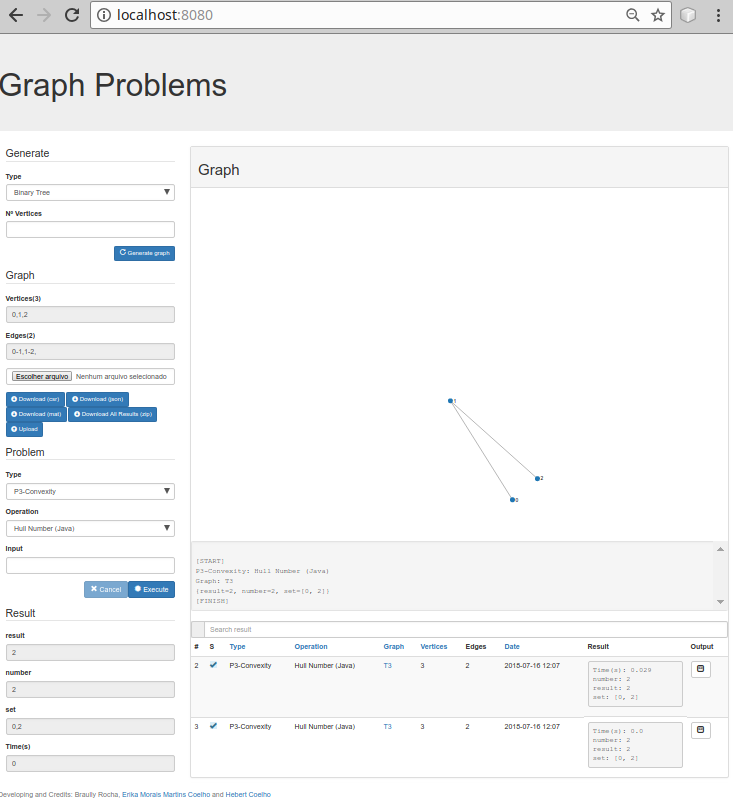
\includegraphics[width=0.8\textwidth]{./imagens/ferramenta-tela-principal.png}
	\end{center}
   	\caption{Ferramenta para Execução de Algoritmos}
    \label{fig-ferramenta-grafo}
\end{figure}

Na Figura~\ref{fig-ferramenta-grafo-tabela-resultados} 
temos a captura de tela da região de histórico de resultados executados.
No histórico é possível buscar resultados anteriores,
filtrar por algum termo, entre as informações apresentadas estão o problema, o grafo informado, a quantidade de vértices e arestas,
tempo de execução e o resultado do problema em si.

\begin{figure}[h]
	\begin{center}
	    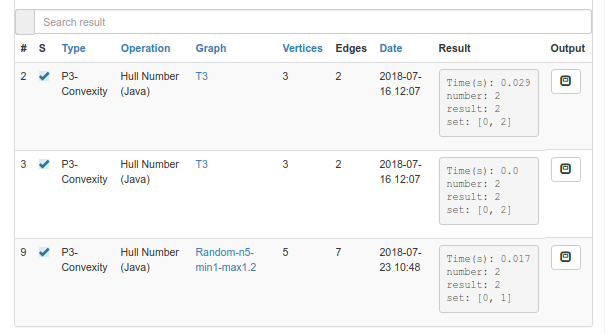
\includegraphics[width=0.8\textwidth]{./imagens/ferramenta-resultado.png}
	\end{center}
	\caption{Captura de Tela Histórico de Resultados}
    \label{fig-ferramenta-grafo-tabela-resultados}
\end{figure}

Na Figura~\ref{fig-ferramenta-grafo-console} temos a captura de tela da área que contem uma representação visual do grafo em uso e um console com as informações de qualquer operação em andamento.

\begin{figure}[H]
\begin{center}
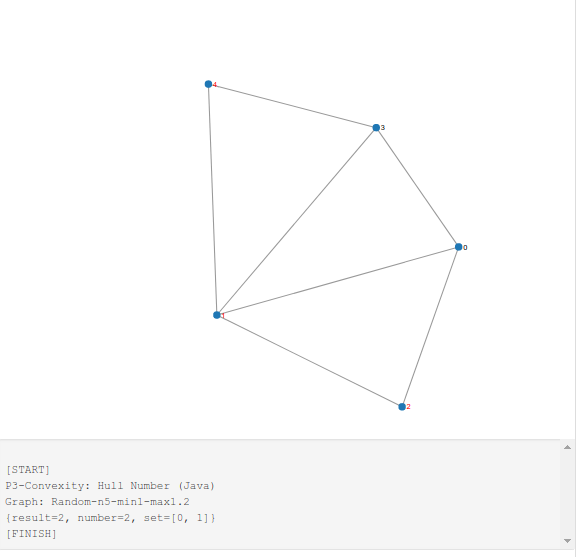
\includegraphics[width=0.5\textwidth]{./imagens/ferramenta-resultado-console.png}
\end{center}
\caption{Captura de Tela Imagem Grafo e Console de Execução}
\label{fig-ferramenta-grafo-console}
\end{figure}


Na Figura~\ref{fig-ferramenta-area-gerador} temos em maior detalhe a captura de tela da área de geração de grafo.

\begin{figure}[H]
	\begin{center}
	    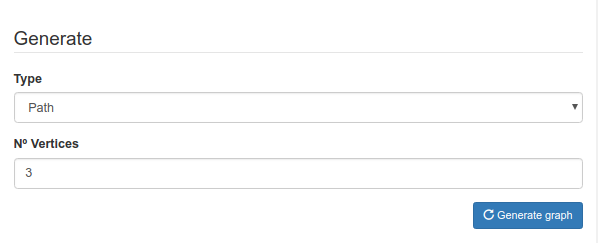
\includegraphics[width=0.5\textwidth]{./imagens/ferramenta-area-gerador.png}
	\end{center}
	\caption{Captura de Tela Geração de Grafo}
    \label{fig-ferramenta-area-gerador}
\end{figure}

Na Figura~\ref{fig-ferramenta-area-info-grafo} temos em maior detalhe a captura de tela da área de informações sobre o grafo.
Temos os vértices, lista de arestas, além dos botões que permitem baixar o grafo atual nos formatos \textit{csr}, \textit{json} e \textit{mat}.
Também está disponível um botão para baixar todos o histórico de resultados. 
Por fim também temos a opção de fazer o \textit{upload} de um arquivo contendo um grafo, nos mesmos formatos disponíveis para \textit{download}.

\begin{figure}[H]
\begin{center}
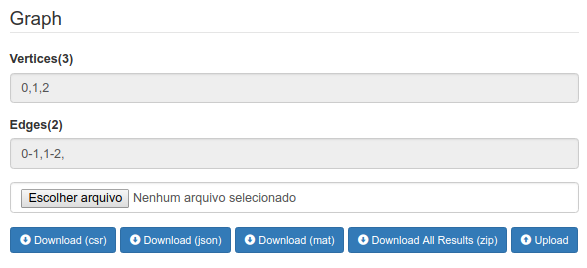
\includegraphics[width=0.5\textwidth]{./imagens/ferramenta-area-info-grafo.png}
\end{center}
\caption{Captura de Tela Geração de Grafo}
\label{fig-ferramenta-area-info-grafo}
\end{figure}


Na Figura~\ref{fig-ferramenta-area-problema} temos em maior detalhe 
a captura de tela da área de seleção do problema e o botão para executar a operação. Para problemas que exigem informações extras de entrada, 
existe uma caixa para digitação dessas informações.

\begin{figure}[H]
\begin{center}
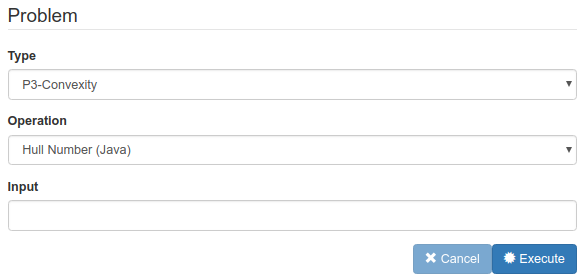
\includegraphics[width=0.5\textwidth]{./imagens/ferramenta-area-problema.png}
\end{center}
\caption{Captura de Tela Seleção de Problema}
\label{fig-ferramenta-area-problema}
\end{figure}



\chapter{Grafo Formato N,M,Índice}
\label{apend-nm-indice}
Neste trabalho grande parte das implementações exigiram combinações para soluções de problemas
e na geração de grafos. Por vezes se fez necessário uma forma simples de retomar a construção de um grafo,
com uma combinação do gerador de grafo completo e uso do índice lexicográfico para obter uma combinação,
elaboramos um gerador/formato de representação de um grafo partindo apenas de três números inteiros.

Considere o Algoritmo~\ref{alg:gera-kn} gerador de um grafo completo simples e não direcionado.
Dado que qualquer grafo de ordem $n$ é subgrafo de $K_n$ apenas removendo arestas. 
Se pudermos identificar na linha $9$ quais arestas não adicionar em $E$, 
o algoritmo pode ser utilizado para gerar qualquer grafo não direcionado. 


\begin{algorithm2e}[H]
    \SetAlFnt{\tiny}
    \SetAlCapFnt{\small}
    \SetAlCapNameFnt{\small}
    \SetAlgoLined
    \DontPrintSemicolon
    \LinesNumbered
    \SetAlgoLined
    \BlankLine
    \Entrada{$n$}
    \Saida{Grafo $G$ completo de ordem $n$}
    \BlankLine
    $V \gets \emptyset$ \\
    $E \gets \emptyset$ \\
    $rotulo \gets 0$ \\
    \Para{$i \gets 0$ \Ate $n-1$}{
    	$V\gets V \cup \{i\}$\\
    }        
    \Para{$i \gets 0$ \Ate $n-1$}{
    	\Para{$j \gets i+1$ \Ate $n-1$}{
    		$E \gets E \cup (i,j)$\\
            $rotulo \gets rotulo + 1$
    	}
    }
    \Retorna{$G(V,E)$} 
\caption{$GeraK_n(n)$}
\label{alg:gera-kn}
\end{algorithm2e} 

No Algoritmo~\ref{alg:gera-kn} sabemos que para uma entrada $n$, será gerado um grafo completo com $n$ vértices e consequentemente $m=\frac{n(n-1)}{2}$ arestas.  Podemos perceber que cada aresta poderia ser identificada de forma única por um rotulo gerado na linha 10. Se existe a priori um conjunto com todos os rótulos de arestas a serem gerados, 
poderia se adicionar em $E$ apenas as arestas desejadas, podendo assim gerar qualquer grafo $G$ de ordem $n$ desejado.


Seja $n$ o número de vértices, sabendo que $MaximoArestas(n)=\frac{n(n-1)}{2}$. Um conjunto contendo $k$ rótulos de arestas desejadas, nada mais é que uma combinação $C(MaximoArestas(n),k)$. Ao passo que qualquer combinação $C(a,b)$ pode ser obtida a partir de seu índice lexicográfico, desde que se conheça os valores de $a$, $b$. Podemos assim representar qualquer grafo de ordem $n$ com apenas 3 números: quantidade de vértices (n), arestas (m) e o índice lexicográfico (i).


Com pequenas alterações no algoritmo de geração de grafo completo podemos obter o Algoritmo~\ref{alg:gera-n}, que é capaz de gerar qualquer grafo a partir de três números inteiros. Vejamos um exemplo, seja $K_5$ o grafo retornado pelo Algoritmo~\ref{alg:gera-kn} para $n=5$, será gerado 10 arestas e com rótulos conforme Figura~\ref{fig-exemplos-algoritmos-geracao}. Os grafos $C_5$ e $W_5$ podem ser obtidos a partir de $K_5$ apenas removendo algumas arestas. Em $C_5$ as arestas desejadas são as de rótulo $R_{C_5}=\{1, 4, 5, 8, 10\}$. Ao passo que as arestas desejadas para se obter um $W_5$ são $R_{W_5}=\{1, 2, 3, 4, 5, 7, 8, 10\}$. A combinação de arestas para o dado $C_5$ é a de índice lexicográfico 99, portanto o mesmo grafo poderia ser gerado pelo Algoritmo~\ref{alg:gera-n} com os parâmetros $n=5$, $m=5$ e $i_{lex}=99$. Ao passo que para o $W_5$ o índice lexicográfico do conjunto de arestas é 32, podendo ser gerado pelo Algoritmo~\ref{alg:gera-n} com os parâmetros $n=5$, $m=8$ e $i_{lex}=32$.

Dado que um conjunto é uma combinação de dois números, esse conjunto pode ser facilmente convertido em um índice lexicográfico. O contrário também se confirma, dado o índice lexicográfico de uma combinação, podemos obter a combinação representada pelo índice. Assim temos uma forma diferente e interessante de se representar grafos.


\begin{algorithm2e}[H]
    \SetAlFnt{\tiny}
    \SetAlCapFnt{\small}
    \SetAlCapNameFnt{\small}
    \SetAlgoLined
    \DontPrintSemicolon
    \LinesNumbered
    \SetAlgoLined
    \BlankLine
    \Entrada{$n$, $m$ e $i_{lex}$}
    \Saida{Grafo $G$ completo de ordem $n$}
    \BlankLine
    $V \gets \emptyset$ \\
    $E \gets \emptyset$ \\
    $R \gets Combinacao(\frac{n(n-1)}{2},k,i_{lex})$\\
    $rotulo \gets 0$ \\
    \Para{$i \gets 0$ \Ate $n-1$}{
    	$V\gets V \cup \{i\}$\\
    }        
    \Para{$i \gets 0$ \Ate $n-1$}{
    	\Para{$j \gets i+1$ \Ate $n-1$}{
        	\Se{$rotulo\in R$} {
    			$E \gets E \cup (i,j)$\\
            }
            $rotulo \gets rotulo + 1$
    	}
    }
    \Retorna{$G(V,E)$} 
\caption{$GeraG(n,m,i_{lex})$}
\label{alg:gera-n}
\end{algorithm2e} 


\begin{figure}[h]
\centering
\begin{tikzpicture}
    \node[draw,circle,label={\small $v_1$}] (v1) at (-6,2) {};
\node[draw,circle,label=$v_2$] (v2) at (-5,1.5) {};
\node[draw,circle,label=below right:$v_3$] (v3) at (-5.5,0) {};
\node[draw,circle,label=below left:$v_4$] (v4) at (-6.5,0) {};
\node[draw,circle,label=$v_5$] (v5) at (-7,1.5) {};

\draw  (v1) -- node {\tiny $1$} (v2);
\draw  (v1) -- node {\tiny $2$}  (v3); 
\draw  (v1) -- node {\tiny $3$}  (v4);
\draw  (v1) -- node {\tiny $4$}  (v5);
\draw  (v2) -- node {\tiny $5$}  (v3);
\draw  (v2) -- node {\tiny $6$}  (v4);
\draw  (v2) -- node {\tiny $7$}  (v5);
\draw  (v3) -- node {\tiny $8$}  (v4);
\draw  (v3) -- node {\tiny $9$}  (v5);
\draw  (v4) -- node {\tiny ${10}$}  (v5);
\node at (-6,-1) {$k_5$};


\node[draw,circle,label={\small $v_1$}] (v21) at (-3,2) {};
\node[draw,circle,label=$v_2$] (v22) at (-2,1.5) {};
\node[draw,circle,label=below right:$v_3$] (v23) at (-2.5,0) {};
\node[draw,circle,label=below left:$v_4$] (v24) at (-3.5,0) {};
\node[draw,circle,label=$v_5$] (v25) at (-4,1.5) {};

\draw  (v21) -- node {\tiny $1$} (v22);
\draw  (v21) -- node {\tiny $4$}  (v25);
\draw  (v22) -- node {\tiny $5$}  (v23);
\draw  (v23) -- node {\tiny $8$}  (v24);
\draw  (v24) -- node {\tiny ${10}$}  (v25);
\node at (-3,-1) {$C_5$};

\node[draw,circle,label={\small $v_1$}] (v31) at (0,0.75) {};
\node[draw,circle,label=$v_2$] (v32) at (1,1.5) {};
\node[draw,circle,label=below:$v_3$] (v33) at (1,0) {};
\node[draw,circle,label=below:$v_4$] (v34) at (-1,0) {};
\node[draw,circle,label=$v_5$] (v35) at (-1,1.5) {};

\draw  (v31) -- node {\tiny $1$} (v32);
\draw  (v31) -- node {\tiny $2$}  (v33); 
\draw  (v31) -- node {\tiny $3$}  (v34);
\draw  (v31) -- node {\tiny $4$}  (v35);
\draw  (v32) -- node {\tiny $5$}  (v33);

\draw  (v32) -- node {\tiny $7$}  (v35);
\draw  (v33) -- node {\tiny $8$}  (v34);
\draw  (v34) -- node {\tiny ${10}$}  (v35);
\node at (0,-1) {$W_5$};
\end{tikzpicture}
\caption{Grafos gerados pelos Algoritmos~\ref{alg:gera-kn} e~\ref{alg:gera-n}} 
\label{fig-exemplos-algoritmos-geracao}
\end{figure}



% \chapter{Conjecturas e Ensaios de Demonstração}
% Neste apêndice apresentamos algumas ideias exploradas em cima das conjecturas investigadas, apesar de não concluídos os estudos, deixamos aqui para registro e futuros trabalhos.

% % \begin{conjecture}
% %     Seja $G$ um grafo com diâmetro 2, então $c(G) \le 4$.
% %     \label{conjecture-g-c4}
% % \end{conjecture}

% % \begin{conjecture}
% %     Seja $G$ um grafo e $d$ seu diâmetro, então $c(G) \le d^2$.
% %     \label{conjecture-d2-c4}
% % \end{conjecture}

% % \begin{conjecture}
% %     Seja $G$ um grafo com diâmetro 2, sem vértice de corte então $h(G) \le 4$.
% %     \label{conjecture-d2-4}
% % \end{conjecture}

% A Conjectura~\ref{conjecture-d2-4} foi a mais investigada no decorrer do trabalho, permanecendo em aberta  e exigem mais investigação, dois possíveis caminhos mais promissores para a demonstração estão apresentados aqui. 


% No primeiro caminho usando a propriedade de dominação total da vizinhança de qualquer vértice de um grafo de diâmetro 2, juntamente com o principio da casa do pombos, segue uma possível demonstração.    
%     Seja $v_1$ um vértice de $G$, tal que $d(v_1)=\Delta(G)$. Faça $S_1=\{v_1\}$, $H(S_1)$ e $R_1=V(G) \setminus N(H(S_1))$, se $R_1$ é vazio então $S_1$ é dominante, caso contrário sabemos que $R_1 < n-\Delta$. Se $S_1$ não é envoltório então pelo principio da casa dos pombos existe um vértice $v_2$, tal que $d(v_2) \ge \lceil \frac{n-\Delta}{\Delta} \rceil$. Faça $S_2=\{v_1,v_2\}$, $H(S_2)$ e $R_2=V(G) \setminus N(H(S_2))$, se $R_2$ é dominante então $|S_2|+1$ é envoltório, sabemos então que $R_2 < n - \Delta - \lceil \frac{n-\Delta}{\Delta} \rceil$. Se $S_2$ não é envoltório então pelo principio da casa dos pombos existe um vértice $v_3$, tal que $d(v_3) \ge \lceil \frac{n-\Delta - \lceil \frac{n-\Delta}{\Delta} \rceil }{\Delta-1} \rceil$ e assim sucessivamente, podemos estabelecer uma relação de recorrência para o conjunto $R_i=n-T(i-1)$ tal que: 
    
%      $$
%       T(0) = \Delta 
%       T(i) =  \Big\lceil \frac{\Delta - i - 1}{\Delta-i} \times (T(i-1)+n) \Big\rceil 
%     $$
%     Em um grafo cujo $\Delta$ seja elevado, $R_i$ será vazio em poucas iterações, tal como $\Delta=n-2$ em que o $R_i$ será zero na segunda iteração. Porém quando $\Delta$ assume o minimo valor possível, mais iterações são necessárias. Pelas propriedades de um grafo diâmetro 2 minimal, o menor valor possível para $\Delta$ é $\sqrt[]{n-1}$ substituindo esse valor na equação de recorrência, e resolvendo a equação, é possível saber para qualquer grafo de ordem $n$ em qual iteração $i$ o valor de $R_i \le 0$. Se encerrar em uma constante, temos assim o primeiro possível caminho de demonstração da conjectura.
    
% Em uma possível demonstração mais direta, baseada apenas nas propriedades de que para qualquer dois vértices em um grafo de diâmetro 2, ou são vizinhos ou tem um vizinho em comum. Segue um outro possível caminho de demonstração.
% 	Se $G$ é um grafo de diâmetro 2, necessariamente existem pelo menos dois vértices não adjacentes. Caso contrário, $G$ seria um grafo completo e um grafo completo possui diâmetro é 1.
    
%     Seja $v_1,v_2\in V(G)$ dois vértices distintos e não adjacentes. Como $G$ é um grafo de diâmetro 2 então existe um vértice $z \in V(G)$ tal que $v_1z, v_2z \in E(G)$. Considere $S_1=\{v_1, v_2\}$. Note que $z \in H(S_1)$. Agora, vamos separar os vértices de $G$ em dois conjuntos, $H(S_1)$ e $V(G) \setminus H(S_1)$. 
    
%     Como não existe vértice de corte em G, $v_1$ e $v_2$ possuem outros vizinhos, não necessariamente em comum, diferentes de $z$. Se $N(u) \subseteq H(S_1)$, $u \in H(S_1)$, então pela Proposição \ref{pro-diam-2-itemb} $H(S_1)$ é um conjunto dominante. Logo pelo Lema \ref{hs-dominante-envoltorio} $S_1 \cup \{v\}$ é um conjunto envoltório, para $v \in V(G) \setminus H(S_1)$. Portanto $h(G)\le 3$.
    
%     Agora, considere que todo vértice de $H(S_1)$ possua pelo menos um vizinho em $V(G) \setminus H(\{S_1\})$. Note que não existe $v \in V(G) \setminus H(\{S_1\})$ que pertença a vizinhança de quaisquer dois vértices de $H(S_1)$. Caso contrário, $v$ pertenceria a $H(S_1)$. 
    
%     Considere $v_3 \in V(G) \setminus H(\{S_1\})$ tal que $v_2v_3 \in E(G)$. Faça $S_2=\{v_1, v_2, v_3\}$. Observe que $v_1v_3 \notin E(G)$, então existe um vértice $u \in V(G) \setminus H(\{S_1\})$ tal que $uv_1, uv_3 \in E(G)$. Dessa forma existe um ciclo de tamanho cinco, $C=v_1, z, v_2, v_3, u$. Caso $V(G)\setminus H(S_2)=\emptyset$ então $h(G)\le 3$.
    
% %    Caso $V(G) \setminus H(S_2) \ne \emptyset$. Se $V(G) \setminus N(H(S_2)) = \emptyset$ então pelo Lema~\ref{hs-dominante-envoltorio} $G$ tem um conjunto envoltório $S_2\cup \{v\}$, logo $h(G)\le 4$. Caso $V(G) \setminus N(H(S_2)) \ne \emptyset$ e $\exists v \in V(G) \H(S_2) | N(v) \subset N(H(S))$ então pelo Lema~\ref{hs-dominante-envoltorio} $G$ tem um conjunto envoltório $S_2\cup \{v\}$, logo $h(G)\le 4$.

%      Caso $V(G) \setminus H(S_2) \ne \emptyset$. Se $V(G) \setminus N(H(S_2)) = \emptyset$ então pelo Lema~\ref{hs-dominante-envoltorio} $G$ tem um conjunto envoltório $S_2\cup \{v\}$, logo $h(G)\le 4$.  Caso $V(G) \setminus N(H(S_2)) \ne \emptyset$ e $\exists v \in V(G) \setminus H(S_2) | N(v) \subset N(H(S))$ então pelo Lema~\ref{hs-dominante-envoltorio} $G$ tem um conjunto envoltório $S_2\cup \{v\}$, logo $h(G) \le 4$.
    
%     Permanecendo em aberto o caso final em que $\forall v \in V(G)\setminus N(H(S_2))$ v é adjacente a outro vértice em $V(G) \setminus N(H(S_2))$. Conjuntos $H=H(S_2)$, $N=N(H(S_2)) \setminus H(S_2)$ e $R=V(G) \setminus N(H(S_2))$. Para este ultimo caso, segue as observações levantadas:
%      \begin{itemize}
%      \item{Observação-1: Todo vértice $v$ em $R$ possui $|H(S)|$ de seus vizinhos em $N$. Esse vértices de $v$ em $N$ possuem grau minimo $|H(S)|$ }
%      \item{Observação-2: Os vértices adjacente de $v$ que também estejam em $R$ possuem grau minimo 5.}
%      \item{Observação-4: Para todo vértice $v$ em $R$: Pela casa dos pombos $N[v]$ domina $N-N[v]$ e existe um vértice de grau $\frac{|N|-|H(S)|}{d(v)}$ .}
%      \item{Observação-5: Os vértices adjacente de $v$ que também estejam em $R$ precisam dominar $N(C_5)$.}
%      \end{itemize}
     
% %Todo vértice $v$ em $R$ pode ter no máximo $x$ vizinhos em $R$. Sendo $x=\lceil\frac{|N|-|H(S)}{\Delta-1}\rceil$. E o grau minimo de $v$ é $d(v) \ge |H(S)|+\lceil\frac{|N|-|H(S)}{\Delta-1}\rceil$

% %Sabemos que $d(v)=\Delta$. Desenvolvendo a expressão

% %$d(v) \ge |H(S)|+\lceil\frac{|N|-|H(S)}{\Delta-1}\rceil \le \Delta$

% %$d(v) \ge \lceil\frac{|N|-(\Delta-2)|H(S)}{\Delta-1}\rceil \le \Delta$

% %$\lceil\frac{|N|-(\Delta-2)|H(S)}{\Delta-1}\rceil \le \Delta$





\end{document}

